% Yap technical report: architecture, data flow and features of the Yap mobile app.
%
% Build from this folder with Tectonic, which fetches the packages it needs:
%
%   tectonic yapmap-technical-report.tex
%
% Section text lives in sections/, diagram sources in figures/, shared styles in preamble.tex.

\documentclass[11pt, openany]{report}
% Packages, page design, colours and the macros used throughout the report.

% Inline code keeps its spaces and may break at them.
\PassOptionsToPackage{obeyspaces, spaces}{url}

% ---------------------------------------------------------------- fonts
\usepackage{fontspec}
\setmainfont{texgyrepagella}[
  Extension = .otf,
  UprightFont = *-regular,
  BoldFont = *-bold,
  ItalicFont = *-italic,
  BoldItalicFont = *-bolditalic,
]
\setsansfont{texgyreheros}[
  Extension = .otf,
  UprightFont = *-regular,
  BoldFont = *-bold,
  ItalicFont = *-italic,
  BoldItalicFont = *-bolditalic,
  Scale = MatchLowercase,
]
\setmonofont{lmmono10-regular.otf}[
  BoldFont = lmmonolt10-bold.otf,
  ItalicFont = lmmono10-italic.otf,
  Scale = MatchLowercase,
]
\linespread{1.06}
\usepackage{microtype}

% ---------------------------------------------------------------- page
\usepackage[letterpaper, top=26mm, bottom=28mm, inner=28mm, outer=28mm, headsep=9mm, footskip=12mm]{geometry}
\setlength{\parindent}{0pt}
\setlength{\parskip}{0.55\baselineskip plus 2pt minus 1pt}
\clubpenalty=10000
\widowpenalty=10000
\tolerance=1500
\emergencystretch=3em

% ---------------------------------------------------------------- colour
\usepackage{xcolor}
\definecolor{ink}{HTML}{1C1917}
\definecolor{muted}{HTML}{57534E}
\definecolor{rule}{HTML}{A8A29E}
\definecolor{hairline}{HTML}{D6D3D1}
\definecolor{panel}{HTML}{F5F2EE}
\definecolor{accent}{HTML}{15803D}
\definecolor{accentsoft}{HTML}{DCFCE7}
\definecolor{accentdark}{HTML}{166534}
\definecolor{alert}{HTML}{B91C1C}
\definecolor{alertsoft}{HTML}{FEE2E2}
\definecolor{server}{HTML}{E7EEF7}
\definecolor{serverline}{HTML}{3B5B7F}
\color{ink}

% ---------------------------------------------------------------- headings
\usepackage{titlesec}
\titleformat{\chapter}[display]
  {\sffamily\bfseries\color{ink}}
  {\large\color{accent}Chapter \thechapter}
  {6pt}
  {\LARGE}
  [\vspace{4pt}{\color{hairline}\titlerule[0.6pt]}]
\titleformat{name=\chapter, numberless}[display]
  {\sffamily\bfseries\color{ink}}
  {}
  {0pt}
  {\LARGE}
  [\vspace{4pt}{\color{hairline}\titlerule[0.6pt]}]
\titlespacing*{\chapter}{0pt}{0pt}{22pt}
\titleformat{\section}
  {\sffamily\bfseries\large\color{ink}}{\color{accent}\thesection}{0.8em}{}
\titlespacing*{\section}{0pt}{18pt plus 4pt minus 2pt}{6pt}
\titleformat{\subsection}
  {\sffamily\bfseries\normalsize\color{ink}}{\color{accent}\thesubsection}{0.8em}{}
\titlespacing*{\subsection}{0pt}{12pt plus 3pt minus 2pt}{4pt}
\titleformat{\paragraph}[runin]
  {\sffamily\bfseries\small\color{ink}}{}{0pt}{}[.]
\titlespacing*{\paragraph}{0pt}{6pt plus 2pt}{0.6em}
\setcounter{secnumdepth}{2}
\setcounter{tocdepth}{1}

% ---------------------------------------------------------------- running heads
\usepackage{fancyhdr}
\pagestyle{fancy}
\fancyhf{}
\renewcommand{\headrulewidth}{0pt}
\renewcommand{\chaptermark}[1]{\markboth{#1}{}}
\fancyhead[L]{\sffamily\footnotesize\color{muted}Yap technical report}
\fancyhead[R]{\sffamily\footnotesize\color{muted}\leftmark}
\fancyfoot[C]{\sffamily\footnotesize\color{muted}\thepage}
\fancypagestyle{plain}{\fancyhf{}\fancyfoot[C]{\sffamily\footnotesize\color{muted}\thepage}}

% ---------------------------------------------------------------- lists, tables, floats
\usepackage{enumitem}
\setlist{itemsep=2pt, topsep=2pt, parsep=0pt, leftmargin=1.4em}
\setlist[description]{font=\normalfont\bfseries, itemsep=3pt, leftmargin=1.4em}
\usepackage{booktabs}
\usepackage{array}
\usepackage{colortbl}
\usepackage{tabularx}
\usepackage{longtable}
\renewcommand{\arraystretch}{1.18}
\setlength{\tabcolsep}{5pt}
\newcolumntype{L}[1]{>{\raggedright\arraybackslash}p{#1}}
\newcolumntype{Y}{>{\raggedright\arraybackslash}X}
\usepackage{caption}
\captionsetup{font={small,sf}, labelfont={bf,color=ink}, labelsep=period, justification=raggedright, singlelinecheck=false, skip=6pt}
\captionsetup[table]{position=top}
\usepackage{float}
\setlength{\textfloatsep}{14pt plus 3pt minus 3pt}
\setlength{\floatsep}{12pt plus 3pt minus 3pt}
\renewcommand{\topfraction}{0.9}
\renewcommand{\bottomfraction}{0.7}
\renewcommand{\textfraction}{0.08}
\renewcommand{\floatpagefraction}{0.8}

% Smaller table text, used inside every table environment.
\newcommand{\tablefont}{\small}

% ---------------------------------------------------------------- code
\usepackage{listings}
\lstdefinelanguage{pgsql}{
  language=SQL,
  morekeywords={returns,language,security,definer,plpgsql,declare,begin,end,raise,exception,
    if,then,elsif,else,found,returning,conflict,do,nothing,coalesce,least,exists,interval,
    jsonb_build_object,perform,using,policy,for,to,with,check,replace,function,stable,immutable,
    true,false,null,not,and,or,in,is,set,search_path,new,old},
  sensitive=false,
}
\lstset{
  basicstyle=\ttfamily\footnotesize,
  keywordstyle=\color{accentdark}\bfseries,
  commentstyle=\color{muted}\itshape,
  stringstyle=\color{serverline},
  columns=fullflexible,
  keepspaces=true,
  breaklines=true,
  breakatwhitespace=true,
  frame=single,
  framerule=0pt,
  backgroundcolor=\color{panel},
  xleftmargin=6pt,
  xrightmargin=6pt,
  framexleftmargin=6pt,
  framexrightmargin=6pt,
  framextopmargin=4pt,
  framexbottommargin=4pt,
  aboveskip=8pt,
  belowskip=8pt,
  showstringspaces=false,
  upquote=true,
}

% ---------------------------------------------------------------- diagrams
\usepackage{tikz}
\usetikzlibrary{arrows.meta, positioning, calc, fit, backgrounds, shapes.geometric, shapes.multipart, matrix}
% Shared TikZ styles and the small macro set used to draw sequence diagrams.

\tikzset{
  >={Stealth[length=2.1mm, width=1.6mm]},
  every picture/.style={line cap=round, line join=round},
  % boxes
  box/.style={draw=rule, fill=white, rounded corners=1.5pt, font=\sffamily\small, align=center,
    inner xsep=5pt, inner ysep=4pt, minimum height=7mm},
  % colour variants: combine with box, or with a style built on it
  clientbox/.style={fill=panel},
  serverbox/.style={draw=serverline, fill=server},
  accentbox/.style={draw=accent, fill=accentsoft},
  layer/.style={draw=hairline, fill=white, rounded corners=3pt, inner sep=7pt},
  layerlabel/.style={font=\sffamily\scriptsize\bfseries, text=muted, anchor=north west, inner sep=3pt},
  % lines
  flow/.style={->, draw=ink, line width=0.55pt},
  softflow/.style={->, draw=muted, line width=0.5pt, dashed},
  edgelabel/.style={font=\sffamily\scriptsize, fill=white, inner sep=1.5pt, text=ink},
  % state machines
  state/.style={draw=accent, fill=accentsoft, rounded corners=7pt, font=\sffamily\small\bfseries,
    minimum height=8mm, minimum width=19mm, align=center, text=accentdark},
  endstate/.style={state, draw=rule, fill=panel, text=ink},
  startdot/.style={circle, fill=ink, inner sep=0pt, minimum size=2.2mm},
  transition/.style={->, draw=ink, line width=0.55pt},
  translabel/.style={font=\sffamily\scriptsize, fill=white, inner sep=1.5pt, align=center, text=ink},
  % flowcharts
  step/.style={box, text width=#1, inner ysep=5pt},
  step/.default=34mm,
  decision/.style={draw=accent, fill=accentsoft, diamond, aspect=2.2, inner sep=1pt,
    font=\sffamily\scriptsize, align=center, text=accentdark},
  terminal/.style={box, rounded corners=8pt, fill=panel},
  % entity-relationship diagrams
  entity/.style={rectangle split, rectangle split parts=2, draw=rule, fill=white,
    rectangle split part fill={panel, white}, font=\ttfamily\scriptsize, align=flush left,
    inner xsep=4pt, inner ysep=2.5pt, text width=#1, rounded corners=1pt},
  entity/.default=36mm,
  privateentity/.style={entity=#1, dashed},
  privateentity/.default=36mm,
  relation/.style={draw=muted, line width=0.5pt},
  card/.style={font=\sffamily\scriptsize, text=muted, inner sep=1pt},
  % sequence diagrams
  actor/.style={draw=rule, fill=panel, rounded corners=1.5pt, font=\sffamily\scriptsize\bfseries,
    align=center, minimum height=8mm, minimum width=19mm, inner xsep=3pt, anchor=south},
  serveractor/.style={actor, draw=serverline, fill=server},
  lifeline/.style={draw=hairline, line width=0.6pt},
  call/.style={->, draw=ink, line width=0.5pt},
  reply/.style={->, draw=muted, line width=0.5pt, dash pattern=on 2.2pt off 1.6pt},
  push/.style={->, draw=accent, line width=0.6pt},
  msglabel/.style={font=\sffamily\scriptsize, text=ink, above, inner sep=1.2pt, align=center, fill=white, fill opacity=0.9, text opacity=1},
  seqnote/.style={draw=hairline, fill=white, font=\sffamily\scriptsize, align=center,
    inner xsep=4pt, inner ysep=2.5pt, rounded corners=1pt, text=muted},
  fragment/.style={draw=rule, line width=0.45pt, fill=panel!45},
  fraglabel/.style={draw=rule, fill=white, font=\sffamily\scriptsize\bfseries, inner sep=2pt},
  fragguard/.style={font=\sffamily\scriptsize\itshape, text=muted, inner sep=2pt},
}

% \participant[style]{node name}{x in cm}{label}
\newcommand{\participant}[4][actor]{\node[#1] (#2) at (#3,0) {#4};}

% \lifelines{y bottom in cm}{comma-separated node names}, drawn behind everything else.
\newcommand{\lifelines}[2]{%
  \begin{scope}[on background layer]
    \foreach \p in {#2} {\draw[lifeline] (\p.south) -- (\p |- 0,-#1);}
  \end{scope}}

% \msg[style]{from}{to}{y in cm}{label}: a horizontal message between two lifelines.
\newcommand{\msg}[5][call]{\draw[#1] (#2 |- 0,-#4) -- (#3 |- 0,-#4) node[msglabel, midway] {#5};}

% \selfmsg{participant}{y in cm}{label}: a call a participant makes to itself.
\newcommand{\selfmsg}[3]{%
  \draw[call] (#1 |- 0,-#2) -- ++(0.32,0) -- ++(0,-0.3) -- ++(-0.32,0);
  \node[font=\sffamily\scriptsize, anchor=west, align=left, inner sep=1pt, fill=white, fill opacity=0.9, text opacity=1] at ($(#1 |- 0,-#2)+(0.4,-0.15)$) {#3};}

% \seqnote{left participant}{right participant}{y in cm}{text}: a note spanning lifelines.
\newcommand{\seqnote}[4]{%
  \path let \p1=(#1), \p2=(#2) in
    node[seqnote, anchor=north, minimum width={\x2-\x1+12mm}] at ({(\x1+\x2)/2}, -#3 cm) {#4};}

% \fragment{left participant}{right participant}{y top}{y bottom}{label}: a combined fragment.
\newcommand{\fragment}[5]{%
  \begin{scope}[on background layer]
    \draw[fragment] ($(#1 |- 0,-#3)+(-1.05,0)$) rectangle ($(#2 |- 0,-#4)+(1.05,0)$);
  \end{scope}
  \node[fraglabel, anchor=north west] at ($(#1 |- 0,-#3)+(-1.05,0)$) {#5};}

% \fragsep{left participant}{right participant}{y}{guard}: a dashed divider inside a fragment.
\newcommand{\fragsep}[4]{%
  \draw[rule, dash pattern=on 3pt off 2pt, line width=0.45pt]
    ($(#1 |- 0,-#3)+(-1.05,0)$) -- ($(#2 |- 0,-#3)+(1.05,0)$);
  \node[fragguard, anchor=north west] at ($(#1 |- 0,-#3)+(-1.0,0)$) {#4};}

% \fragguardat{left participant}{y}{guard}: the guard of a fragment's first operand.
\newcommand{\fragguardat}[3]{\node[fragguard, anchor=north west] at ($(#1 |- 0,-#2)+(-1.0,0)$) {#3};}


% ---------------------------------------------------------------- boxes
\usepackage[skins, breakable]{tcolorbox}

% ---------------------------------------------------------------- links and references
\usepackage[hidelinks, bookmarksnumbered, pdfusetitle]{hyperref}
\hypersetup{
  pdftitle={Yap technical report},
  pdfsubject={Architecture, data flow and features of the Yap mobile app},
  pdfkeywords={Yap, YapMap, Expo, React Native, Supabase, PostGIS, row-level security},
}
\usepackage[nameinlink, capitalise, noabbrev]{cleveref}
\crefname{lstlisting}{Listing}{Listings}
\Crefname{lstlisting}{Listing}{Listings}

% Inline code: identifiers, file paths and values. Breaks are allowed after underscores,
% slashes, dots and hyphens, so long names never run into the margin.
\DeclareUrlCommand\codeurl{\urlstyle{tt}}
\DeclareRobustCommand{\code}{\codeurl}
\makeatletter
\g@addto@macro\UrlBreaks{\do\_\do\-\do\.\do\/\do\(\do\)}
\makeatother

% Screen and interface labels, as the app shows them.
\newcommand{\ui}[1]{\textsf{#1}}

% A defined term at the point where it is introduced.
\newcommand{\term}[1]{\emph{#1}}

% A short remark set off from the text, with a lead-in label: \begin{remark}{Label} ... \end{remark}.
\newtcolorbox{remark}[1]{
  enhanced, breakable,
  colback=panel, colframe=panel, boxrule=0pt, arc=0pt,
  left=8pt, right=8pt, top=5pt, bottom=5pt,
  borderline west={2pt}{0pt}{accent},
  before skip=8pt, after skip=8pt,
  fontupper=\small,
  before upper={\textsf{\textbf{#1.}}\enskip},
}

% Where a feature lives: \implemented{screens}{client functions}{server rules}.
\newcommand{\implemented}[3]{%
  \par\vspace{2pt}\begingroup\small\setlength{\tabcolsep}{4pt}\renewcommand{\arraystretch}{1.12}%
  \noindent\begin{tabularx}{\linewidth}{@{}>{\sffamily\bfseries\footnotesize\color{muted}}L{15mm}Y@{}}
    \arrayrulecolor{hairline}\hline
    Screens & #1 \\
    Client & #2 \\
    Server & #3 \\
    \hline
  \end{tabularx}\endgroup\par\vspace{2pt}}


\begin{document}

\pagenumbering{alph}
% Title page, summary, contents and lists of figures and tables.

\begin{titlepage}
  \thispagestyle{empty}
  \vspace*{30mm}
  {\sffamily\bfseries\fontsize{40}{44}\selectfont\color{accent}Yap\par}
  \vspace{6mm}
  {\sffamily\bfseries\LARGE Technical report\par}
  \vspace{4mm}
  {\sffamily\large\color{muted}Architecture, data flow and features of the Yap mobile app\\and its Supabase backend\par}
  \vspace{10mm}
  {\color{accent}\rule{28mm}{1.2pt}\par}
  \vspace{10mm}
  {\small
  \begin{tabular}{@{}L{34mm}L{100mm}@{}}
    \textsf{\textbf{Subject}} & The YapMap repository, branch \code{main} after pull request 74 and the migration renames (October 2026) \\
    \textsf{\textbf{Platforms}} & iOS and Android (Expo SDK 57, React Native 0.86) \\
    \textsf{\textbf{Backend}} & Supabase: Postgres with PostGIS, Auth, Realtime, Storage and \code{pg_cron} \\
    \textsf{\textbf{Course}} & COMP 2160 (Section 01), Mobile App Development 1, final project \\
    \textsf{\textbf{Team}} & Samar Khajuria and Manik Singh \\
    \textsf{\textbf{Date}} & October 2026 \\
  \end{tabular}\par}
  \vfill
  {\footnotesize\color{muted}
  Copyright \textcopyright{} 2026 Samar Khajuria. All rights reserved. The software described here and its
  source code are proprietary and may not be used, copied, modified or distributed without the written
  permission of the copyright holder.\par}
\end{titlepage}
\pagenumbering{roman}

\chapter*{Summary}
\addcontentsline{toc}{chapter}{Summary}
\markboth{Summary}{}

Yap is a mobile app that helps people who share a physical space, such as a café or a campus lounge,
start a conversation in person. A user goes live for 30, 60 or 120 minutes, sees the other live users
within about 100 metres, and sends one of them a request to talk. If the request is accepted within five
minutes, the two users enter a private chat that exists to help them find each other and meet. Users can
also place small public events on a map, which anyone within 5 kilometres can join, each with its own
group chat.

The client is a single Expo and React Native code base written in TypeScript. Expo Router maps files to
screens; one store in \code{src/state/store.ts} holds all shared state and owns every Realtime
subscription; and one module, \code{src/data/api.ts}, makes every call to the backend. The backend is a
Supabase project with no application server. Postgres row-level security denies direct access by default,
and every write other than the user's own profile columns, an unblock and the user's own photo files
goes through a \code{SECURITY DEFINER} database function that derives the caller from the session and
checks what that action needs: identity, state, proximity, blocks or rate limits. PostGIS answers the proximity
questions, Realtime delivers requests and messages, a private Storage bucket holds photos behind
short-lived signed URLs, and a \code{pg_cron} job ends expired sessions, requests and stale chats every
minute.

Privacy shapes the design throughout. Live positions are written once per session, are never returned to
any client, and are deleted the moment a user goes offline. Other users see a person card that carries a
first name and last initial but no location or distance. A photo can be loaded only by someone who can
currently see its owner. The project accepted one deliberate trade-off to keep the promise that a location
is deleted on going offline: the server cannot rate-limit the distance between two separate live
sessions, so it limits how often a location may change instead.

Safety follows the app stores' rules for apps where people post and meet. Every user agrees to community
guidelines at sign-up, can report and block from every screen that shows another person, and cannot post
slurs or abusive words, which the database refuses. The owner reviews reports at least daily and can
suspend an account. Continuous integration checks the app, the migration files and a database rebuilt
from every migration on each pull request, and store builds are made with EAS Build.

This report describes the architecture (\cref{ch:architecture}), the data model (\cref{ch:data-model})
and the server interface (\cref{ch:server-interface}); traces each major flow with sequence diagrams
(\cref{ch:flows}); catalogues every feature with the screens, functions and server rules that implement
it (\cref{ch:features}); and covers security and privacy, reliability, performance, configuration,
validation, and known limitations in the chapters that follow.

\clearpage
{\hypersetup{linkcolor=ink}\tableofcontents}
\clearpage
\listoffigures
\listoftables


\clearpage
\pagenumbering{arabic}
\chapter{Introduction}
\label{ch:introduction}

\section{Purpose and scope}

This report describes Yap as it exists on the \code{main} branch of the YapMap repository at commit
\code{9271c80}. It covers the architecture of the mobile client and its backend, the data model, the
flow of data through the system, every user-facing feature, and the rules the server enforces. It is
written for engineers who maintain, review or extend the app, and for readers who need to understand
what the app does with personal data.

Every statement in the report is taken from the source code, the SQL migrations in
\code{supabase/migrations}, the repository documentation and the history of merged pull requests. Where
behaviour depends on configuration that lives outside the repository, such as settings in the Supabase
dashboard, the report says so. Numbers such as radii, time limits and rate limits are quoted from the
code that enforces them; \cref{tab:parameters} collects them in one place.

The report is organised in three parts. \Cref{ch:architecture,ch:data-model,ch:server-interface}
describe the structure of the system: its components, its data and the interface between client and
server. \Cref{ch:flows,ch:features} describe behaviour: the major flows step by step, then each feature
with the screens and functions that implement it. \Cref{ch:security,ch:reliability,ch:performance,ch:configuration,ch:testing,ch:limitations}
cover cross-cutting qualities and operations. A glossary and three reference appendices close the report.

\section{What Yap does}

Yap is a mobile app for iOS and Android that helps people in the same place have a spontaneous
conversation in person. The product line on its welcome screen states the intent: \emph{the app that gets
you off the app}. The app is built around a short, repeated loop:

\begin{enumerate}
  \item \textbf{Go live.} A user taps the large \ui{YAP} button, chooses how long to be visible (30, 60 or
    120 minutes) and may add a note of up to 60 characters, such as where to find them. The phone sends
    its position once, and the user becomes \term{live}.
  \item \textbf{See who is nearby.} While live, the user sees a list of the other live users within about
    100 metres. The list shows a photo, first name and last initial, the note, an introduction and
    interests. It never shows a location or a distance.
  \item \textbf{Say hi.} The user opens one person's profile and sends a \term{say-hi request}. The
    recipient has five minutes to answer. A sender can have only one request waiting at a time.
  \item \textbf{Accept or decline.} The recipient sees the sender's full profile and two buttons of
    equal weight, \ui{Accept} and \ui{Not now}. A declined request and an expired request look the same
    to the sender, who sees \ui{Not this time}.
  \item \textbf{Chat and meet.} An accepted request opens a private one-to-one chat. While they chat, both
    users disappear from everyone else's nearby list. The chat exists so the two can find each other in
    the room.
  \item \textbf{End.} Either user ends the chat and records whether they met. If they are still live, both
    return to the nearby lists.
\end{enumerate}

Alongside the loop, the \ui{Map} tab shows \term{events}: small public plans, such as a coffee or a study
break, that a host places at a chosen spot. Anyone within 5 kilometres of an event can join it, and every
member can read and write its group chat. \Cref{fig:core-loop} shows the loop and the event path.

\begin{figure}[t]
  \centering
  % The core loop and the event path (Figure: core loop).
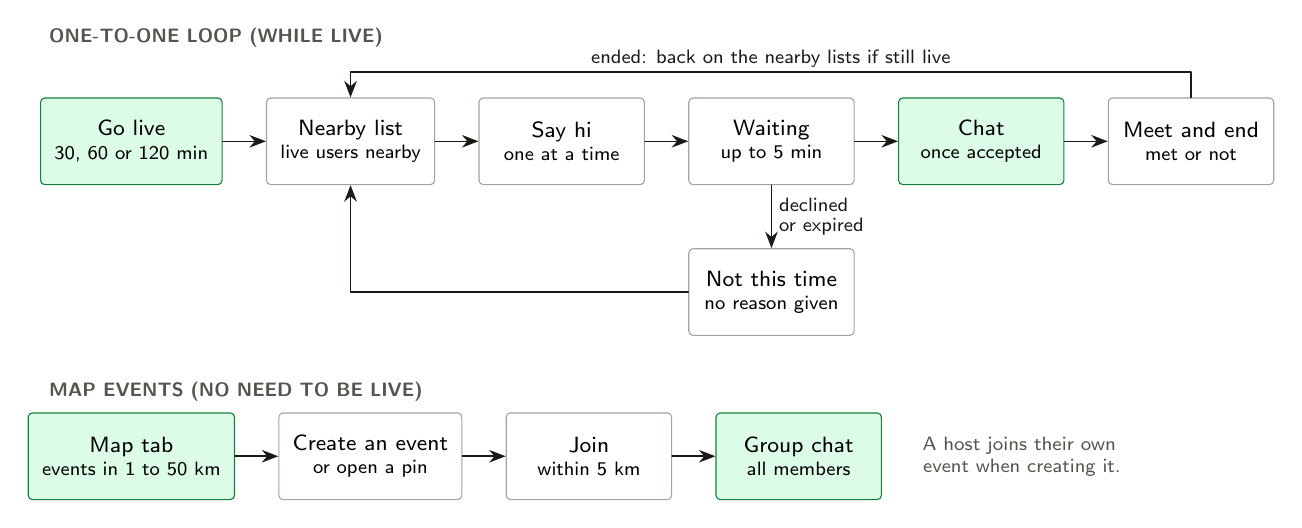
\begin{tikzpicture}[
    node distance=5.5mm,
    loopbox/.style={box, minimum width=21mm, minimum height=11mm, font=\sffamily\footnotesize},
    sub/.style={font=\sffamily\scriptsize, text=muted},
  ]
  \node[layerlabel, inner sep=0pt] at (-1.05,1.45) {ONE-TO-ONE LOOP (WHILE LIVE)};
  \node[loopbox, accentbox] (live) at (0,0) {Go live\\[-1pt]{\scriptsize 30, 60 or 120 min}};
  \node[loopbox, right=of live] (nearby) {Nearby list\\[-1pt]{\scriptsize live users nearby}};
  \node[loopbox, right=of nearby] (hi) {Say hi\\[-1pt]{\scriptsize one at a time}};
  \node[loopbox, right=of hi] (wait) {Waiting\\[-1pt]{\scriptsize up to 5 min}};
  \node[loopbox, accentbox, right=of wait] (chat) {Chat\\[-1pt]{\scriptsize once accepted}};
  \node[loopbox, right=of chat] (end) {Meet and end\\[-1pt]{\scriptsize met or not}};
  \node[loopbox, below=8mm of wait] (no) {Not this time\\[-1pt]{\scriptsize no reason given}};

  \draw[flow] (live) -- (nearby);
  \draw[flow] (nearby) -- (hi);
  \draw[flow] (hi) -- (wait);
  \draw[flow] (wait) -- (chat);
  \draw[flow] (chat) -- (end);
  \draw[flow] (wait) -- node[edgelabel, right=1pt, fill=none, align=left] {declined\\[-1pt]or expired} (no);
  \draw[flow] (no.west) -| (nearby.south);
  \draw[flow] (end.north) -- ++(0,0.32) -| node[edgelabel, pos=0.25, above=0pt, fill=none] {ended: back on the nearby lists if still live} (nearby.north);

  \node[layerlabel, inner sep=0pt] at (-1.05,-3.05) {MAP EVENTS (NO NEED TO BE LIVE)};
  \node[loopbox, accentbox] (map) at (0,-4.0) {Map tab\\[-1pt]{\scriptsize events in 1 to 50 km}};
  \node[loopbox, right=of map] (pin) {Create an event\\[-1pt]{\scriptsize or open a pin}};
  \node[loopbox, right=of pin] (join) {Join\\[-1pt]{\scriptsize within 5 km}};
  \node[loopbox, accentbox, right=of join] (group) {Group chat\\[-1pt]{\scriptsize all members}};
  \draw[flow] (map) -- (pin);
  \draw[flow] (pin) -- (join);
  \draw[flow] (join) -- (group);
  \node[sub, right=4mm of group, align=left, text width=30mm] {A host joins their own event when creating it.};
\end{tikzpicture}

  \caption{The core loop. The upper path is the one-to-one loop; the lower path is the map event feature,
    which does not require being live.}
  \label{fig:core-loop}
\end{figure}

\section{Design principles}

Five principles recur throughout the code. They explain many of the decisions described later.

\begin{description}
  \item[Locations are never shown.] The server returns people, never positions or distances. A live
    position is stored only while the user is live and is never sent back to any client. The only places
    the app shows are event locations, which hosts choose on purpose (\cref{sec:location-privacy}).
  \item[The server enforces every rule.] The client cannot write to any table except its own profile row
    and its own block list. Every other write goes through a database function that checks who is calling,
    what state they are in, whether the two people are near each other or have blocked each other, and
    whether a rate limit applies. A modified client cannot bypass these checks (\cref{ch:security}).
  \item[One thing at a time.] A sender has at most one request waiting, and a user takes part in at most
    one chat. While a request or chat is on screen, further incoming requests are not shown and expire on
    the server.
  \item[No pressure.] Declining is as easy as accepting, and the sender cannot tell a decline from an
    expiry. The interface uses the phrase \ui{Not this time} for both.
  \item[Safety is two taps away.] Every surface that shows another person carries a menu with
    \ui{Report} and \ui{Block}. A block takes effect on the server at once, in both directions.
\end{description}

\section{Conventions}

The report uses the following conventions.

\begin{itemize}
  \item \code{Monospace} marks identifiers, file paths, SQL and values as they appear in the code.
    Paths are relative to the repository root. \ui{Sans-serif} marks labels the app shows on screen.
  \item A \term{database function} is a Postgres function in the \code{public} schema that the client
    calls through the Supabase API (a remote procedure call, or RPC). A \term{helper} is a function in
    the \code{private} schema, which clients cannot call. The \term{caller} is the signed-in user on whose
    behalf a database function runs; functions read the caller's identity from the session with
    \code{auth.uid()} and never accept it as an argument.
  \item A \term{store action} is an exported function in \code{src/state/store.ts}. An \term{API function}
    is an exported function in \code{src/data/api.ts}.
  \item Distances are in metres unless stated otherwise. The client represents instants as milliseconds
    since the Unix epoch; the database stores \code{timestamptz} values and converts them to
    milliseconds in the JSON it returns.
  \item Terms with a specific meaning in Yap, such as \term{live}, \term{open}, \term{chatting},
    \term{person card} and \term{catch-up}, are defined where they first appear and collected in the
    glossary (\cref{ch:glossary}).
\end{itemize}

\section{Key parameters}

\Cref{tab:parameters} lists the limits and timings that define Yap's behaviour, with the place that
enforces each one. Where the client and the server both apply a limit, the server's check is the one that
cannot be bypassed.

\begingroup\tablefont
\begin{longtable}{@{}L{40mm}L{48mm}L{\dimexpr\linewidth-88mm-4\tabcolsep\relax}@{}}
  \caption{Key parameters and where they are enforced.}
  \label{tab:parameters}\\
  \toprule
  \textsf{\textbf{Parameter}} & \textsf{\textbf{Value}} & \textsf{\textbf{Enforced by}} \\
  \midrule
  \endfirsthead
  \toprule
  \textsf{\textbf{Parameter}} & \textsf{\textbf{Value}} & \textsf{\textbf{Enforced by}} \\
  \midrule
  \endhead
  \bottomrule
  \endfoot
  \multicolumn{3}{@{}l}{\textsf{\textbf{Going live and nearby}}} \\
  Live duration & 30, 60 or 120 minutes & \code{go_green}; \code{DURATIONS} in \code{constants.ts} \\
  Live note length & 0 to 60 characters & check constraint; \code{go_green}, \code{update_note} \\
  Nearby radius & 100\,m plus the caller's reported GPS accuracy, at most 150\,m & \code{nearby}, \code{private.near_each_other} \\
  Nearby list size & at most 50 people & \code{nearby} \\
  Nearby refresh & every 20\,s while live and on screen & \code{NEARBY_REFRESH_MS}, \code{useNearbyPolling} \\
  Location changes & at most 3 in any 10 minutes & \code{go_green} \\
  Movement while live & at most 150\,m plus 10\,km/h since the position was set & \code{go_green} \\
  GPS wobble & moves of 150\,m or less are ignored & \code{go_green} \\
  \midrule
  \multicolumn{3}{@{}l}{\textsf{\textbf{Requests and chats}}} \\
  Answer window & 5 minutes & default of \code{chat_requests.expires_at} \\
  Requests sent & at most 5 in any 10 minutes & \code{send_request} \\
  Requests waiting per sender & 1 & partial unique index; \code{send_request} \\
  Chats per user & 1 & \code{send_request}, \code{respond} \\
  Message length & 1 to 1000 characters & check constraint; both send functions \\
  Messages sent & at most 30 per minute, one-to-one and group combined & \code{send_chat_message}, \code{send_event_message} \\
  Chat history loaded & newest 200 messages & \code{HISTORY_LIMIT} in \code{api.ts} \\
  \midrule
  \multicolumn{3}{@{}l}{\textsf{\textbf{Events}}} \\
  Map radius & 1 to 50\,km, default 10\,km & slider and \code{EVENT_RADIUS_KM}; \code{events_near} caps at 50\,km \\
  Visibility after start & 3 hours & \code{events_near} \\
  Start time & now to 7 days ahead (server allows 5 minutes in the past) & event form; \code{create_event} \\
  Events created & at most 5 per host in any 24 hours & \code{create_event} \\
  Events listed & at most 50 & \code{events_near} \\
  Join distance & within 5\,km & \code{join_event} \\
  Title and description & 1 to 60 and 0 to 200 characters & check constraints; form limits \\
  \midrule
  \multicolumn{3}{@{}l}{\textsf{\textbf{Profiles and photos}}} \\
  Names & 1 to 30 characters each & check constraints; form limits \\
  Introduction & 1 to 300 characters & check constraint; form limit \\
  Interests & 3 to 5 & check constraint; setup and edit forms \\
  Extra photos & 4 to 6 in the app; at most 6 on the server & forms; \code{profiles_photo_paths_max} \\
  Uploaded photo & JPEG, at most 1080\,px wide, quality 0.8 & \code{uploadJpeg} \\
  Avatar copy & JPEG, 320\,px wide & \code{uploadJpeg} \\
  Storage object & at most 5\,MiB; JPEG, PNG or WebP & \code{photos} bucket settings \\
  Signed photo URL & valid 1 hour; reused until 10 minutes remain & \code{SIGNED_URL_SECONDS}, \code{SIGNED_URL_MIN_LEFT_MS} \\
  \midrule
  \multicolumn{3}{@{}l}{\textsf{\textbf{Accounts and safety}}} \\
  Password & at least 8 characters & \code{PASSWORD_MIN_LENGTH}; Supabase Auth setting \\
  Emailed code & 8 digits; resend after 60\,s & email templates; \code{verify.tsx} \\
  Automatic hiding & 3 distinct reporters & \code{report_user} \\
  Report details & at most 500 characters & \code{report_user}; check constraint \\
  Housekeeping & every minute & \code{pg_cron} job \code{yap-expire-stale} \\
\end{longtable}
\endgroup

\chapter{System architecture}
\label{ch:architecture}

Yap has two tiers: a native mobile client and a hosted Supabase project. There is no application server
of Yap's own. Business rules live in the database, as row-level security policies and as database
functions; Supabase provides authentication, a REST interface to the database, Realtime delivery,
file storage and scheduled jobs around it. This chapter describes both tiers and the boundary between
them. \Cref{fig:architecture} gives the overall picture.

\begin{figure}[ht]
  \centering
  % System architecture: client layers and Supabase services (Figure: architecture).
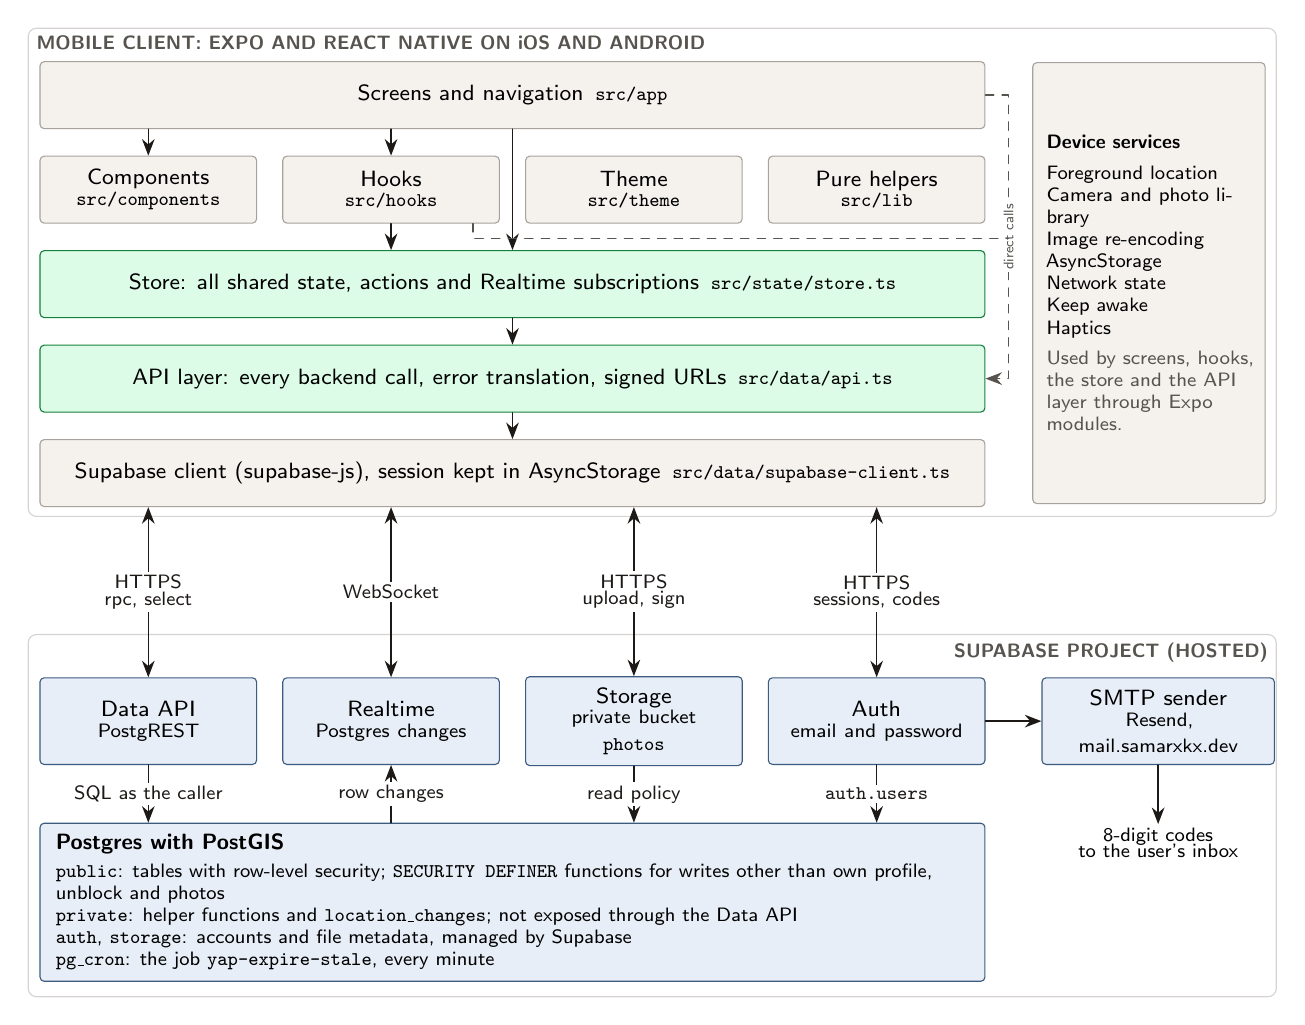
\begin{tikzpicture}[
    band/.style={box, clientbox, minimum height=8.5mm, font=\sffamily\footnotesize},
    svc/.style={box, serverbox, minimum height=11mm, text width=24mm, font=\sffamily\footnotesize},
    path/.style={font=\ttfamily\scriptsize, text=muted},
    proto/.style={font=\sffamily\scriptsize, text=ink, fill=white, inner sep=1.2pt, align=center},
  ]
  % ---------------------------------------------------------------- client
  \begin{scope}[on background layer]
    \node[layer, fit={(-0.15,0.85) (15.7,-5.35)}, inner sep=0pt] (clientframe) {};
  \end{scope}
  \node[layerlabel] at (clientframe.north west) {MOBILE CLIENT: EXPO AND REACT NATIVE ON iOS AND ANDROID};

  \node[band, minimum width=12cm] (screens) at (6,0) {Screens and navigation\enskip{\ttfamily\scriptsize src/app}};
  \node[band, minimum width=2.75cm] (components) at (1.375,-1.2) {Components\\[-2pt]{\ttfamily\scriptsize src/components}};
  \node[band, minimum width=2.75cm] (hooks) at (4.458,-1.2) {Hooks\\[-2pt]{\ttfamily\scriptsize src/hooks}};
  \node[band, minimum width=2.75cm] (theme) at (7.542,-1.2) {Theme\\[-2pt]{\ttfamily\scriptsize src/theme}};
  \node[band, minimum width=2.75cm] (lib) at (10.625,-1.2) {Pure helpers\\[-2pt]{\ttfamily\scriptsize src/lib}};
  \node[band, accentbox, minimum width=12cm] (store) at (6,-2.4) {Store: all shared state, actions and Realtime subscriptions\enskip{\ttfamily\scriptsize src/state/store.ts}};
  \node[band, accentbox, minimum width=12cm] (api) at (6,-3.6) {API layer: every backend call, error translation, signed URLs\enskip{\ttfamily\scriptsize src/data/api.ts}};
  \node[band, minimum width=12cm] (client) at (6,-4.8) {Supabase client (supabase-js), session kept in AsyncStorage\enskip{\ttfamily\scriptsize src/data/supabase-client.ts}};

  \node[box, clientbox, text width=26mm, align=left, font=\sffamily\scriptsize, minimum height=5.6cm, anchor=north west] (device) at (12.6,0.42)
    {\textbf{Device services}\\[3pt]
     Foreground location\\
     Camera and photo library\\
     Image re-encoding\\
     AsyncStorage\\
     Network state\\
     Keep awake\\
     Haptics\\[3pt]
     {\color{muted}Used by screens, hooks, the store and the API layer through Expo modules.}};

  \draw[flow] (screens.south -| components) -- (components);
  \draw[flow] (screens.south -| hooks) -- (hooks);
  \draw[flow] (hooks.south) -- (hooks |- store.north);
  \draw[flow] (6,0 |- screens.south) -- (6,0 |- store.north);
  \draw[flow] (store) -- (api);
  \draw[softflow] (screens.east) -- (12.3,0 |- screens.east) -- (12.3,0 |- api.east)
    node[pos=0.5, rotate=90, fill=white, inner sep=1pt, font=\sffamily\tiny, text=muted] {direct calls} -- (api.east);
  \draw[softflow, -] (5.5,0 |- hooks.south) -- (5.5,-1.82) -- (12.3,-1.82);
  \draw[flow] (api) -- (client);

  % ---------------------------------------------------------------- Supabase
  \begin{scope}[on background layer]
    \node[layer, fit={(-0.15,-6.85) (15.7,-11.45)}, inner sep=0pt] (serverframe) {};
  \end{scope}
  \node[layerlabel, anchor=north east] at (serverframe.north east) {SUPABASE PROJECT (HOSTED)};

  \node[svc] (rest) at (1.375,-7.95) {Data API\\[-2pt]{\scriptsize PostgREST}};
  \node[svc] (realtime) at (4.458,-7.95) {Realtime\\[-2pt]{\scriptsize Postgres changes}};
  \node[svc] (storage) at (7.542,-7.95) {Storage\\[-2pt]{\scriptsize private bucket \texttt{photos}}};
  \node[svc] (auth) at (10.625,-7.95) {Auth\\[-2pt]{\scriptsize email and password}};
  \node[svc, text width=26mm] (smtp) at (14.2,-7.95) {SMTP sender\\[-2pt]{\scriptsize Resend, mail.samarxkx.dev}};

  \node[box, serverbox, minimum width=12cm, text width=11.6cm, align=flush left, font=\sffamily\scriptsize] (pg) at (6,-10.25)
    {\textbf{\footnotesize Postgres with PostGIS}\\[2pt]
     \texttt{public}: tables with row-level security; \texttt{SECURITY DEFINER} functions for writes other than own profile, unblock and photos\\
     \texttt{private}: helper functions and \texttt{location\_changes}; not exposed through the Data API\\
     \texttt{auth}, \texttt{storage}: accounts and file metadata, managed by Supabase\\
     \texttt{pg\_cron}: the job \texttt{yap-expire-stale}, every minute};

  \draw[flow, <->] (client.south -| rest) -- node[proto] {HTTPS\\[-2pt]rpc, select} (rest);
  \draw[flow, <->] (client.south -| realtime) -- node[proto] {WebSocket} (realtime);
  \draw[flow, <->] (client.south -| storage) -- node[proto] {HTTPS\\[-2pt]upload, sign} (storage);
  \draw[flow, <->] (client.south -| auth) -- node[proto] {HTTPS\\[-2pt]sessions, codes} (auth);
  \draw[flow] (auth) -- (smtp);
  \draw[flow] (smtp.south) -- ++(0,-0.75) node[below, font=\sffamily\scriptsize, align=center, inner sep=1pt] {8-digit codes\\[-2pt]to the user's inbox};

  \draw[flow] (rest) -- node[proto] {SQL as the caller} (rest |- pg.north);
  \draw[flow] (realtime |- pg.north) -- node[proto] {row changes} (realtime);
  \draw[flow] (storage) -- node[proto] {read policy} (storage |- pg.north);
  \draw[flow] (auth) -- node[proto] {\texttt{auth.users}} (auth |- pg.north);
\end{tikzpicture}

  \caption{System architecture. Arrows inside the client show the direction of calls between layers;
    the dashed arrow is the direct calls from a few screens and one hook to the API layer, which bypass the
    store. The client reaches four Supabase services; each service reaches Postgres, where the rules are
    enforced.}
  \label{fig:architecture}
\end{figure}

\section{Technology stack}

\Cref{tab:stack} lists the main technologies and the role each plays. Versions are those pinned in
\code{package.json}.

\begin{table}[ht]
  \centering
  \caption{Technology stack.}
  \label{tab:stack}
  \tablefont
  \begin{tabularx}{\textwidth}{@{}L{34mm}L{48mm}Y@{}}
    \toprule
    \textsf{\textbf{Concern}} & \textsf{\textbf{Technology}} & \textsf{\textbf{Role in Yap}} \\
    \midrule
    App runtime & Expo SDK 57, React Native 0.86.3, React 19.2.3 & One code base for iOS and Android \\
    Language & TypeScript 6.0 in strict mode & All client code; path alias \code{@/} for \code{src/} \\
    Navigation & Expo Router 57 with typed routes & File-based routes, guarded stacks, tabs, sheets and modals \\
    Compilation & React Compiler (Expo experiment) & Automatic memoisation of components \\
    Maps & \code{react-native-maps} 1.27.2 & The \ui{Map} tab, event pins and the radius circle \\
    Animation & Reanimated 4.5, Worklets 0.10 & Press feedback, the pulsing \ui{YAP} button, the mascot \\
    Images & \code{expo-image}, \code{expo-image-picker}, \code{expo-image-manipulator} & Cached display, photo picking and camera, re-encoding before upload \\
    Device & \code{expo-location}, \code{expo-haptics}, \code{expo-keep-awake}, \code{expo-network}, \code{expo-clipboard} & Foreground location, haptics, screen-on while live, connectivity, pasting the emailed code \\
    Local storage & AsyncStorage 2.2 & The Supabase session and per-account preferences \\
    Backend client & \code{@supabase/supabase-js} 2.117 & Auth, database calls, Realtime and Storage \\
    Database & Postgres with PostGIS and \code{pg_cron} & Tables, row-level security, functions, spatial queries, housekeeping \\
    Backend services & Supabase Auth, Realtime, Storage & Sign-in and email codes, live delivery, private photos \\
    Email delivery & Custom SMTP through Resend & Sends the 8-digit confirmation and reset codes \\
    Tooling & ESLint 9 with \code{eslint-config-expo}; ImageMagick 7 & Linting; generating icons and splash images \\
    \bottomrule
  \end{tabularx}
\end{table}

\section{Client architecture}
\label{sec:client-architecture}

The client is organised in layers, each in its own directory under \code{src/}
(\cref{tab:client-layers}). Calls flow downward: screens use components, hooks and store actions; the
store calls the API layer; the API layer is the only code that uses the Supabase client.

\begin{table}[ht]
  \centering
  \caption{Client layers.}
  \label{tab:client-layers}
  \tablefont
  \begin{tabularx}{\textwidth}{@{}L{36mm}Y@{}}
    \toprule
    \textsf{\textbf{Directory}} & \textsf{\textbf{Responsibility}} \\
    \midrule
    \code{src/app} & Routes and screens. A file is a route; a \code{_layout.tsx} file is a navigator. Screens hold form state locally and read shared state through \code{useStore}. \\
    \code{src/components} & Shared components grouped by purpose: \code{ui} (buttons, cards, fields, lists, skeletons), \code{profile}, \code{live}, \code{chat}, \code{safety}, \code{events}, \code{account} and \code{mascot}. \\
    \code{src/hooks} & The shared one-second clock and countdowns, foreground location, nearby polling and nearby prompts, and lazy signing of a person's extra photos. \\
    \code{src/state} & The store (\code{store.ts}), the profile-setup draft (\code{profile-draft.tsx}) and per-account preferences saved on the phone (\code{saved-prefs.ts}). \\
    \code{src/data} & The API layer (\code{api.ts}), the single Supabase client (\code{supabase-client.ts}), the data shapes (\code{types.ts}), fixed lists and limits (\code{constants.ts}) and the types generated from the database schema (\code{database.types.ts}). \\
    \code{src/lib} & Pure helpers with no React: wording for names, genders and times, event categories, password checks, error text, image cache keys, tidying typed text, checking picked photos, and the server-corrected clock. \\
    \code{src/theme} & Design tokens (colours for light and dark mode, spacing, radii, sizes, type, elevation, motion) and the \code{useTheme} hook. \\
    \code{src/config} & Feature flags (\code{features.ts}) and the Supabase project address and publishable key (\code{supabase.ts}). \\
    \bottomrule
  \end{tabularx}
\end{table}

\paragraph{Layering rule} No screen or component imports the Supabase client. Most screens change
state only through store actions. A few screens that need no shared state call the API layer directly:
the code entry screen (to resend a code), \ui{Sign in} (to resend a confirmation code), \ui{Forgot
password} and \ui{Change password}. The hook \code{usePersonPhotos} also calls the API layer, to sign a
person's extra photos when their profile opens.

\section{Navigation and route guards}
\label{sec:navigation}

Expo Router turns the files under \code{src/app} into a navigation tree (\cref{fig:routes}). The root
layout, \code{src/app/_layout.tsx}, renders one stack with four \term{guarded} children. A guard is a
Boolean computed from the store; Expo Router allows a protected stack only while its guard is true, so
the app always lands on the correct step without explicit redirects (\cref{tab:guards}).

\begin{figure}[ht]
  \centering
  % Route tree and the guards of the root stack (Figure: routes).
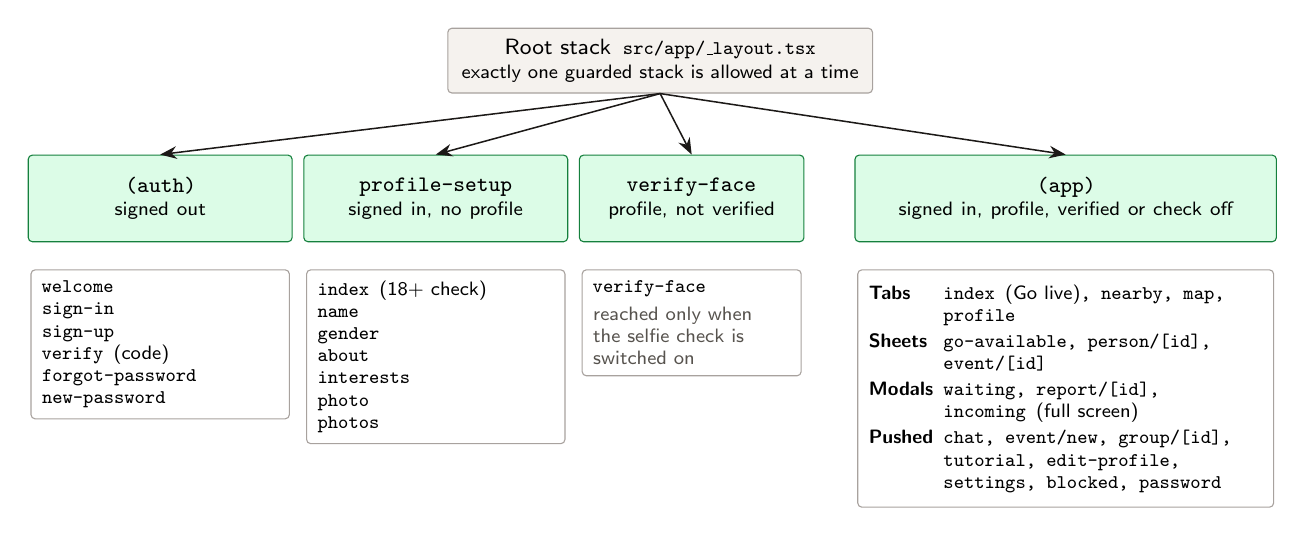
\begin{tikzpicture}[
    stackbox/.style={box, accentbox, font=\sffamily\footnotesize, align=center, minimum height=11mm},
    routes/.style={box, font=\ttfamily\scriptsize, align=flush left, anchor=north, inner sep=4pt},
    guard/.style={font=\sffamily\scriptsize, text=accentdark, align=center},
  ]
  \node[box, clientbox, font=\sffamily\footnotesize] (root) at (7.9,0)
    {Root stack\enskip{\ttfamily\scriptsize src/app/\_layout.tsx}\\[-1pt]{\scriptsize exactly one guarded stack is allowed at a time}};

  \node[stackbox, text width=30mm] (auth) at (1.55,-1.75) {\texttt{(auth)}\\[-1pt]{\scriptsize signed out}};
  \node[stackbox, text width=30mm] (setup) at (5.05,-1.75) {\texttt{profile-setup}\\[-1pt]{\scriptsize signed in, no profile}};
  \node[stackbox, text width=25mm] (verify) at (8.3,-1.75) {\texttt{verify-face}\\[-1pt]{\scriptsize profile, not verified}};
  \node[stackbox, text width=50mm] (app) at (13.05,-1.75) {\texttt{(app)}\\[-1pt]{\scriptsize signed in, profile, verified or check off}};

  \foreach \n in {auth, setup, verify, app} {\draw[flow] (root.south) -- (\n.north);}

  \node[routes, text width=30mm] at (1.55,-2.65)
    {welcome\\sign-in\\sign-up\\verify {\sffamily(code)}\\forgot-password\\new-password};
  \node[routes, text width=30mm] at (5.05,-2.65)
    {index {\sffamily(18+ check)}\\name\\gender\\about\\interests\\photo\\photos};
  \node[routes, text width=25mm] at (8.3,-2.65)
    {verify-face\\[2pt]{\sffamily\color{muted} reached only when\\ the selfie check is\\ switched on}};
  \node[routes, text width=50mm] at (13.05,-2.65)
    {\begin{tabular}{@{}>{\sffamily\bfseries}l@{\enskip}>{\raggedright\arraybackslash}p{38mm}@{}}
       Tabs & index {\sffamily(Go live)}, nearby, map, profile \\[1pt]
       Sheets & go-available, person/[id], event/[id] \\[1pt]
       Modals & waiting, report/[id], incoming {\sffamily(full screen)} \\[1pt]
       Pushed & chat, event/new, group/[id], tutorial, edit-profile, settings, blocked, password \\
     \end{tabular}};
\end{tikzpicture}

  \caption{The route tree. The four children of the root stack are mutually exclusive; the guard under
    each name states when it is allowed. Not drawn: the two unguarded reading pages, \code{guidelines} and
    \code{acknowledgements}.}
  \label{fig:routes}
\end{figure}

\begin{table}[ht]
  \centering
  \caption{Root guards. \emph{Verified} is true when the profile is verified or the selfie check is
    switched off, which is the current setting.}
  \label{tab:guards}
  \tablefont
  \begin{tabularx}{\textwidth}{@{}L{30mm}L{58mm}Y@{}}
    \toprule
    \textsf{\textbf{Stack}} & \textsf{\textbf{Guard}} & \textsf{\textbf{Purpose}} \\
    \midrule
    \code{(auth)} & not signed in & Welcome, sign-up, sign-in, emailed codes, password reset \\
    \code{profile-setup} & signed in and no profile row & The 18+ confirmation and six setup steps \\
    \code{account-restricted} & signed in, profile, hidden or suspended & Explains the hold, with the support email, a sign-out and account deletion \\
    \code{verify-face} & signed in, profile, active, not verified & Selfie check (switched off) \\
    \code{(app)} & signed in, profile, active, verified & The app itself \\
    \bottomrule
  \end{tabularx}
\end{table}

Beside the guarded stacks, the root stack has two pages with no guard, \code{guidelines} (the community
guidelines) and \code{acknowledgements} (the open-source licences), so the sign-up screen and Settings can
both open them, signed in or out.

Before the store has restored the session (\code{booted} is false), the root layout renders an empty
view in the background colour. If the user is signed in but the profile could not be loaded
(\code{loadFailed}), it renders the \ui{Can't reach Yap} screen instead of any stack, so an existing user
is never sent into profile setup by a network failure (\cref{sec:offline}). An offline banner is drawn
over every screen while the phone has no connection.

The \code{(app)} layout hosts the four tabs (\ui{Go live}, \ui{Nearby}, \ui{Map}, \ui{Profile}) and every
screen opened from them. It also runs the behaviour that must apply whichever screen is open:

\begin{itemize}
  \item It starts nearby polling and nearby prompts while the user is live (\cref{sec:feature-nearby}).
  \item It sets a timer that takes the user offline when the live session reaches its end time.
  \item It pushes the \ui{incoming} screen when a new request arrives, and the \ui{chat} screen when a
    chat opens, each only once per request or chat.
  \item It opens the tutorial once after a new account saves its first profile.
  \item It shows the nearby prompt (a toast) and keeps the screen awake while the user is live.
\end{itemize}

\Cref{tab:presentations} lists how each screen in \code{(app)} is presented.

\begin{table}[ht]
  \centering
  \caption{Presentation of the screens in the \code{(app)} stack.}
  \label{tab:presentations}
  \tablefont
  \begin{tabularx}{\textwidth}{@{}L{40mm}L{40mm}Y@{}}
    \toprule
    \textsf{\textbf{Route}} & \textsf{\textbf{Presentation}} & \textsf{\textbf{Notes}} \\
    \midrule
    \code{go-available}, \code{person/[id]} & Form sheet, 85\,\% height & Grabber visible \\
    \code{event/[id]} & Form sheet, 75\,\% height & Event details, \ui{Join}; \ui{Delete event} for the host \\
    \code{waiting}, \code{report/[id]} & Modal, slides from the bottom & \\
    \code{incoming} & Full-screen modal & Swipe to dismiss disabled; the user must answer or let it expire \\
    \code{tutorial} & Pushed, fades in & Swipe back disabled \\
    \code{chat}, \code{event/new}, \code{group/[id]}, \code{edit-profile}, \code{settings}, \code{blocked}, \code{password} & Pushed screen & Slides from the right on both platforms \\
    \bottomrule
  \end{tabularx}
\end{table}

\section{State management}
\label{sec:state}

\subsection{The store}

All shared state lives in one module, \code{src/state/store.ts} (\cref{fig:store-flow}). The module holds
a single immutable state object and a set of listeners. A private function, \code{set(patch)}, replaces
the object with a merged copy and notifies every listener. Components read state with
\code{useStore(selector)}, built on React's \code{useSyncExternalStore}, so a component re-renders only
when the slice it selects changes. Nothing outside the module writes state: screens call exported actions,
and the store's own listeners, timers and Realtime handlers call the same actions.
\Cref{app:store} lists every state field and action.

\begin{figure}[ht]
  \centering
  % Store data flow: what triggers actions, what they change, and who reads it (Figure: store flow).
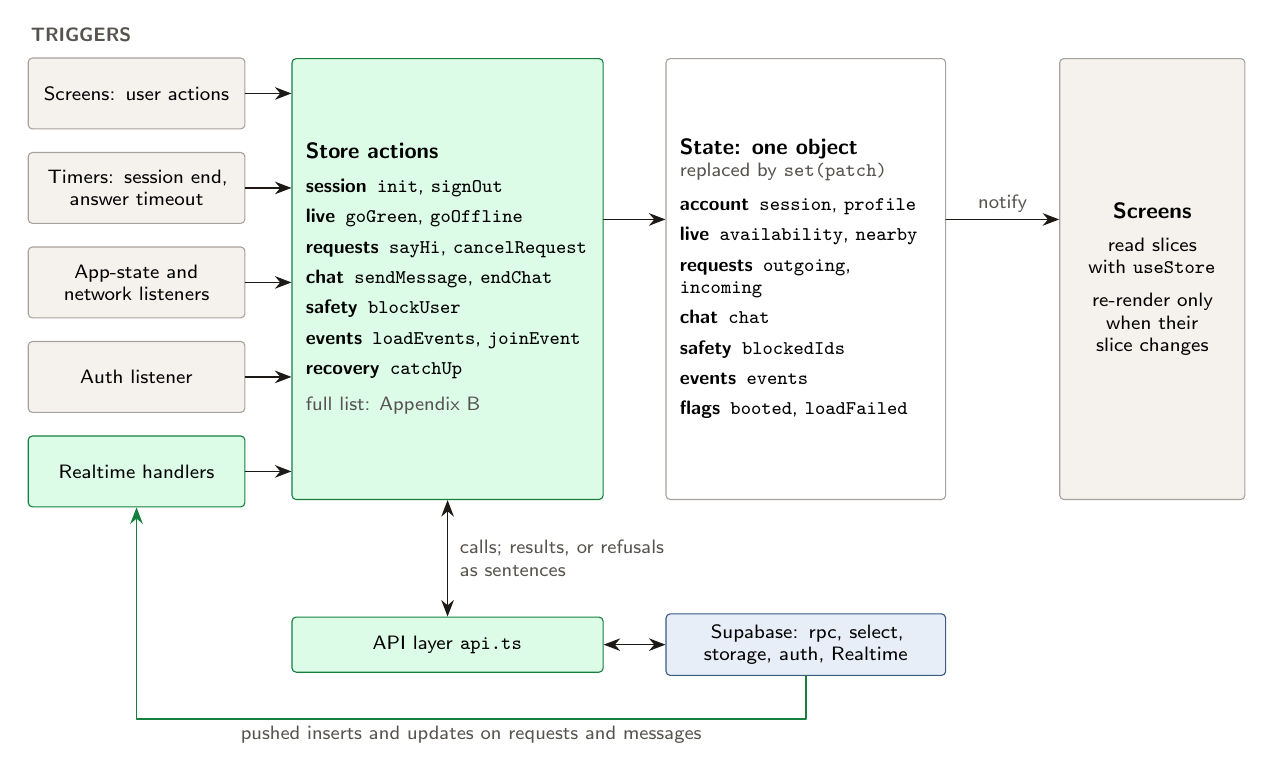
\begin{tikzpicture}[
    inbox/.style={box, clientbox, font=\sffamily\scriptsize, text width=24mm, minimum height=9mm, align=center},
    col/.style={box, font=\sffamily\scriptsize, align=flush left, anchor=north, inner sep=5pt, minimum height=56mm},
    lab/.style={font=\sffamily\scriptsize, text=muted, fill=white, inner sep=1.2pt, align=center},
  ]
  \node[layerlabel, inner sep=0pt, anchor=west] at (0.05,0.75) {TRIGGERS};
  \node[inbox] (ui) at (1.4,0) {Screens: user actions};
  \node[inbox] (timers) at (1.4,-1.2) {Timers: session end,\\answer timeout};
  \node[inbox] (listeners) at (1.4,-2.4) {App-state and\\network listeners};
  \node[inbox] (authl) at (1.4,-3.6) {Auth listener};
  \node[inbox, accentbox] (rt) at (1.4,-4.8) {Realtime handlers};

  \node[col, accentbox, text width=36mm] (actions) at (5.35,0.45)
    {\textbf{\footnotesize Store actions}\\[4pt]
     \textbf{session}\enskip\texttt{init}, \texttt{signOut}\\[3pt]
     \textbf{live}\enskip\texttt{goGreen}, \texttt{goOffline}\\[3pt]
     \textbf{requests}\enskip\texttt{sayHi}, \texttt{cancelRequest}\\[3pt]
     \textbf{chat}\enskip\texttt{sendMessage}, \texttt{endChat}\\[3pt]
     \textbf{safety}\enskip\texttt{blockUser}\\[3pt]
     \textbf{events}\enskip\texttt{loadEvents}, \texttt{joinEvent}\\[3pt]
     \textbf{recovery}\enskip\texttt{catchUp}\\[5pt]
     {\color{muted}full list: Appendix B}};

  \node[col, text width=32mm] (state) at (9.9,0.45)
    {\textbf{\footnotesize State: one object}\\{\color{muted}replaced by \texttt{set(patch)}}\\[4pt]
     \textbf{account}\enskip\texttt{session}, \texttt{profile}\\[3pt]
     \textbf{live}\enskip\texttt{availability}, \texttt{nearby}\\[3pt]
     \textbf{requests}\enskip\texttt{outgoing}, \texttt{incoming}\\[3pt]
     \textbf{chat}\enskip\texttt{chat}\\[3pt]
     \textbf{safety}\enskip\texttt{blockedIds}\\[3pt]
     \textbf{events}\enskip\texttt{events}\\[3pt]
     \textbf{flags}\enskip\texttt{booted}, \texttt{loadFailed}};

  \node[col, clientbox, text width=20mm, align=center] (screens) at (14.3,0.45)
    {\textbf{\footnotesize Screens}\\[4pt]read slices with \texttt{useStore}\\[4pt]re-render only when their slice changes};

  \node[box, accentbox, text width=36mm, font=\sffamily\scriptsize] (api) at (5.35,-7.0) {API layer \texttt{api.ts}};
  \node[box, serverbox, text width=32mm, font=\sffamily\scriptsize] (sb) at (9.9,-7.0) {Supabase: rpc, select,\\storage, auth, Realtime};

  \foreach \n in {ui, timers, listeners, authl, rt} {\draw[flow] (\n.east) -- (\n.east -| actions.west);}
  \draw[flow] (actions.east |- 0,-1.6) -- (state.west |- 0,-1.6);
  \draw[flow] (state.east |- 0,-1.6) -- node[lab, above=1pt] {notify} (screens.west |- 0,-1.6);
  \draw[flow, <->] (actions.south) -- node[lab, right=3pt, fill=none, align=left] {calls; results, or refusals\\as sentences} (api.north);
  \draw[flow, <->] (api) -- (sb);
  \draw[push] (sb.south) -- ++(0,-0.55) -| node[lab, pos=0.25, below=1pt] {pushed inserts and updates on requests and messages} (rt.south);
\end{tikzpicture}

  \caption{Data flow through the store. Five kinds of trigger call actions; actions call the API layer and
    update the one state object; screens re-render from the slices they select. Realtime changes arrive
    as handler calls, like any other trigger.}
  \label{fig:store-flow}
\end{figure}

\subsection{State outside the render tree}

Some state never needs to re-render anything and is kept in module variables inside the store. It
records work in progress and guards against races (\cref{sec:ordering}):

\begin{itemize}
  \item the unsubscribe functions of the three Realtime channels the store may hold open: incoming
    requests, the one-to-one chat, and the open group chat;
  \item \code{handledRequestIds} and \code{closedChatIds}, which stop a catch-up from bringing back a
    request already answered or a chat already closed on this phone;
  \item three counters, \code{nearbyRefreshes}, \code{eventLoads} and \code{eventChatVisits}, which let
    the store discard an answer that arrives after a newer request has started;
  \item flags that coalesce or order work: \code{catchUpRunning}, \code{catchUpAgain},
    \code{offlineRetry}, \code{watchingId}, \code{openingChatId}, \code{extrasLoaded} and
    \code{initStarted}.
\end{itemize}

\subsection{Other client state}

Profile setup keeps its answers in a React context, \code{ProfileDraftProvider}, so the user can move
back and forth between the six steps without losing input. Two preferences are saved on the phone per
account under the AsyncStorage key \code{yap.prefs.<user id>}: how many times the chat safety tip has
been shown, and the map's event radius. Forms keep their field values in component state until they
are submitted.

\section{The API layer}
\label{sec:api-layer}

\code{src/data/api.ts} is the client's only route to the backend. It has four responsibilities.

\begin{description}
  \item[Wrapping calls.] Each exported function wraps one Supabase call or a short sequence of them:
    an Auth method, a database function through \code{supabase.rpc}, a read of a table the user may
    see, or a Storage operation. It converts the JSON the server returns into the client's types in
    \code{types.ts}.
  \item[Translating errors.] A database function refuses a request by raising an exception with a short
    fixed message such as \code{not nearby}. The API layer maps every such message to a sentence for
    the screen through the \code{SERVER_REFUSALS} table, maps Auth error codes in the same way, and
    replaces anything else with a generic sentence, so raw database text never reaches the user
    (\cref{app:refusals}).
  \item[Realtime.] It builds the Realtime channels and subscribes them as the signed-in user
    (\cref{sec:realtime}).
  \item[Photos.] It re-encodes and uploads photos, removes unused files, and turns storage paths into
    signed URLs through a cache (\cref{sec:flow-photos}).
\end{description}

\section{Backend architecture}
\label{sec:backend-architecture}

The backend is one hosted Supabase project. The client knows its URL and its publishable key, both of
which are public by design: the key grants only what row-level security and the database functions
allow. No secret key ships in the app.

\paragraph{Schemas} Yap's database objects span six schemas. \code{public} holds the app's tables and the
database functions the client calls; it is the schema the Data API exposes. \code{private} holds helper
functions and the table \code{location_changes}; it is not exposed. \code{auth} and \code{storage} are
managed by Supabase and hold accounts and file metadata. \code{extensions} holds PostGIS, and
\code{cron} holds the \code{pg_cron} schedule.

\paragraph{Access model} Row-level security is enabled on every application table and denies by default:
a table without a policy cannot be read or written by a client at all. Direct access is granted only
where the client must read rows itself (its own profile, the requests and messages it takes part in, its
own block list) and where a write is trivially safe (its own profile, removing its own block). Every
other write is a \code{SECURITY DEFINER} function: it runs with the privileges of its owner, reads the
caller's identity from \code{auth.uid()}, and checks the rules before changing anything. \Cref{ch:server-interface}
lists the functions and \cref{ch:security} the policies.

\paragraph{Realtime} The tables \code{chat_requests} and \code{messages} are in the
\code{supabase_realtime} publication with full replica identity. Realtime delivers a change to a
subscriber only if the subscriber's token may read the row under the table's select policy, so each user
receives only the requests and messages they take part in.

\paragraph{Storage} Photos live in a private bucket, \code{photos}, under a folder named after the
owner's user ID. Clients write only inside their own folder. Reading, and with it signing a URL, is
allowed only for photos of someone the reader can currently see (\cref{sec:photo-privacy}).

\paragraph{Scheduled work} A \code{pg_cron} job named \code{yap-expire-stale} runs
\code{private.expire_stale()} every minute. It ends live sessions whose time is up, expires unanswered
requests, ends chats in which neither person is live, and prunes the location-change log
(\cref{sec:housekeeping}).

\paragraph{Authentication and email} Supabase Auth provides email and password accounts. \ui{Confirm
email} is switched on, the minimum password length is 8, and the email templates for sign-up
confirmation and password reset show an 8-digit code instead of a link, because the app does not open
email links. Auth sends these emails through a custom SMTP sender, Resend, on the domain
\code{mail.samarxkx.dev}. These settings are made in the Supabase dashboard (\cref{sec:dashboard}).

\chapter{Data model}
\label{ch:data-model}

The database holds eight application tables in the \code{public} schema and one log table in the
\code{private} schema. Every table references \code{profiles}, which has one row per account and itself
references the Supabase Auth user. \Cref{fig:er} shows the tables, their columns and the foreign keys
between them. Every foreign key to a user cascades on delete, so removing an Auth user removes everything
that belongs to that user (\cref{sec:flow-delete}).

\begin{figure}[p]
  \centering
  % Entity-relationship diagram of the database (Figure: entity-relationship).
% Each box lists a table's columns; PK marks the primary key and FK a foreign key. Lines are foreign
% keys, labelled with the referencing columns; 1, n and 0..1 give the cardinality at each end.
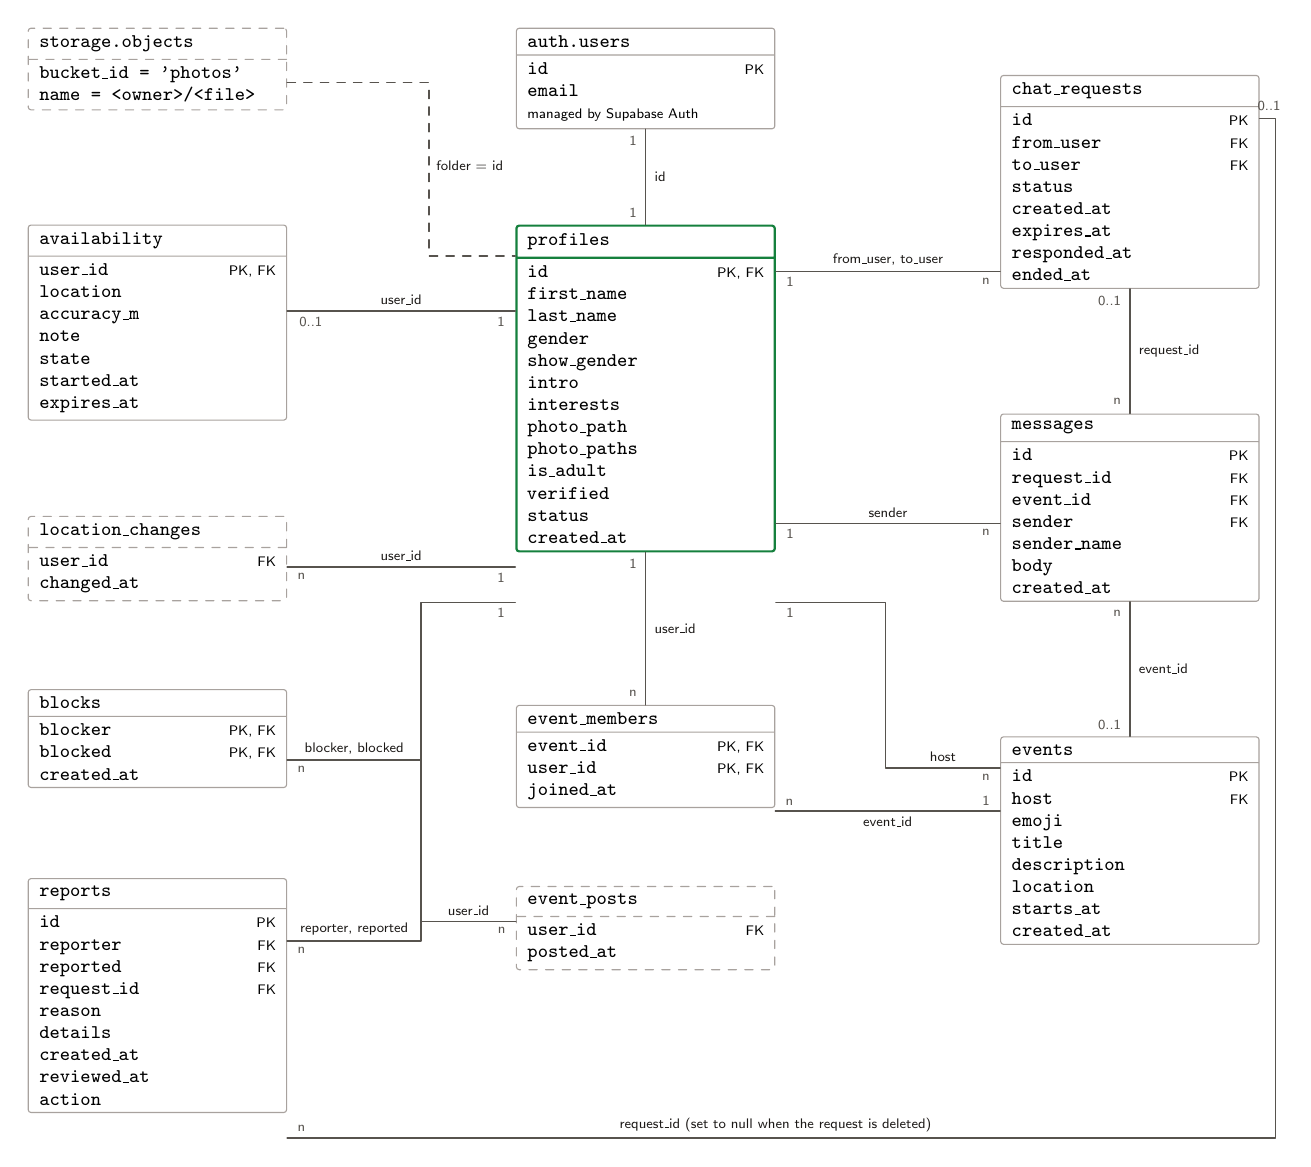
\begin{tikzpicture}[
    k/.style={font=\sffamily\tiny, text=muted, inner sep=1pt},
    kl/.style={font=\sffamily\tiny, text=ink, inner sep=1pt},
  ]
  \newcommand{\pk}{\hfill{\sffamily\tiny PK}}
  \newcommand{\fk}{\hfill{\sffamily\tiny FK}}
  \newcommand{\pkfk}{\hfill{\sffamily\tiny PK, FK}}

  % ---------------------------------------------------------------- column B
  \node[entity=30mm, anchor=north] (users) at (7.95,0) {\textbf{auth.users}\nodepart{two}
    id\pk\\ email\\ {\sffamily\tiny managed by Supabase Auth}};
  \node[entity=30mm, anchor=north, draw=accent, line width=0.8pt] (profiles) at (7.95,-2.5) {\textbf{profiles}\nodepart{two}
    id\pkfk\\ first\_name\\ last\_name\\ gender\\ show\_gender\\ intro\\ interests\\ photo\_path\\
    photo\_paths\\ is\_adult\\ verified\\ status\\ created\_at};
  \node[entity=30mm, anchor=north] (members) at (7.95,-8.6) {\textbf{event\_members}\nodepart{two}
    event\_id\pkfk\\ user\_id\pkfk\\ joined\_at};
  \node[privateentity=30mm, anchor=north] (posts) at (7.95,-10.9) {\textbf{event\_posts}\nodepart{two}
    user\_id\fk\\ posted\_at};

  % ---------------------------------------------------------------- column A
  \node[entity=30mm, anchor=north, dashed] (objects) at (1.75,0) {\textbf{storage.objects}\nodepart{two}
    bucket\_id = 'photos'\\ name = <owner>/<file>};
  \node[entity=30mm, anchor=north] (availability) at (1.75,-2.5) {\textbf{availability}\nodepart{two}
    user\_id\pkfk\\ location\\ accuracy\_m\\ note\\ state\\ started\_at\\ expires\_at};
  \node[privateentity=30mm, anchor=north] (changes) at (1.75,-6.2) {\textbf{location\_changes}\nodepart{two}
    user\_id\fk\\ changed\_at};
  \node[entity=30mm, anchor=north] (blocks) at (1.75,-8.4) {\textbf{blocks}\nodepart{two}
    blocker\pkfk\\ blocked\pkfk\\ created\_at};
  \node[entity=30mm, anchor=north] (reports) at (1.75,-10.8) {\textbf{reports}\nodepart{two}
    id\pk\\ reporter\fk\\ reported\fk\\ request\_id\fk\\ reason\\ details\\ created\_at\\ reviewed\_at\\ action};

  % ---------------------------------------------------------------- column C
  \node[entity=30mm, anchor=north] (requests) at (14.1,-0.6) {\textbf{chat\_requests}\nodepart{two}
    id\pk\\ from\_user\fk\\ to\_user\fk\\ status\\ created\_at\\ expires\_at\\ responded\_at\\ ended\_at};
  \node[entity=30mm, anchor=north] (messages) at (14.1,-4.9) {\textbf{messages}\nodepart{two}
    id\pk\\ request\_id\fk\\ event\_id\fk\\ sender\fk\\ sender\_name\\ body\\ created\_at};
  \node[entity=30mm, anchor=north] (events) at (14.1,-9.0) {\textbf{events}\nodepart{two}
    id\pk\\ host\fk\\ emoji\\ title\\ description\\ location\\ starts\_at\\ created\_at};

  % ---------------------------------------------------------------- relationships
  % profiles - auth.users
  \draw[relation] (users.south) -- node[kl, right=2pt] {id} (profiles.north);
  \node[k, left=2pt] at ($(users.south)+(0,-0.15)$) {1};
  \node[k, left=2pt] at ($(profiles.north)+(0,0.15)$) {1};
  % profiles - storage.objects: by folder name, not a foreign key
  \draw[relation, dashed] (objects.east |- 0,-0.7) -- (5.2,-0.7) |- (profiles.west |- 0,-2.9);
  \node[kl, anchor=west] at (5.25,-1.75) {folder = id};
  % profiles - availability
  \draw[relation] (profiles.west |- 0,-3.6) -- node[kl, above=1pt] {user\_id} (availability.east |- 0,-3.6);
  \node[k, below=1pt] at ($(profiles.west |- 0,-3.6)+(-0.18,0)$) {1};
  \node[k, below=1pt] at ($(availability.east |- 0,-3.6)+(0.3,0)$) {0..1};
  % profiles - location_changes
  \draw[relation] (profiles.west |- 0,-6.85) -- node[kl, above=1pt] {user\_id} (changes.east |- 0,-6.85);
  \node[k, below=1pt] at ($(profiles.west |- 0,-6.85)+(-0.18,0)$) {1};
  \node[k, below=1pt] at ($(changes.east |- 0,-6.85)+(0.18,0)$) {n};
  % profiles - blocks and reports, through one trunk
  \draw[relation] (profiles.west |- 0,-7.3) -- (5.1,-7.3) |- (blocks.east |- 0,-9.3);
  \draw[relation] (5.1,-9.3) |- (reports.east |- 0,-11.6);
  \node[kl, above=1pt] at ($(blocks.east |- 0,-9.3)!0.5!(5.1,-9.3)$) {blocker, blocked};
  \node[kl, above=1pt] at ($(reports.east |- 0,-11.6)!0.5!(5.1,-11.6)$) {reporter, reported};
  \node[k, below=1pt] at ($(profiles.west |- 0,-7.3)+(-0.18,0)$) {1};
  \node[k, below=1pt] at ($(blocks.east |- 0,-9.3)+(0.18,0)$) {n};
  \node[k, below=1pt] at ($(reports.east |- 0,-11.6)+(0.18,0)$) {n};
  % profiles - event_posts, branching from the same trunk
  \draw[relation] (5.1,-11.35) -- node[kl, above=1pt] {user\_id} (posts.west |- 0,-11.35);
  \node[k, below=1pt] at ($(posts.west |- 0,-11.35)+(-0.18,0)$) {n};
  % profiles - chat_requests
  \draw[relation] (profiles.east |- 0,-3.1) -- node[kl, above=1pt] {from\_user, to\_user} (requests.west |- 0,-3.1);
  \node[k, below=1pt] at ($(profiles.east |- 0,-3.1)+(0.18,0)$) {1};
  \node[k, below=1pt] at ($(requests.west |- 0,-3.1)+(-0.18,0)$) {n};
  % profiles - messages
  \draw[relation] (profiles.east |- 0,-6.3) -- node[kl, above=1pt] {sender} (messages.west |- 0,-6.3);
  \node[k, below=1pt] at ($(profiles.east |- 0,-6.3)+(0.18,0)$) {1};
  \node[k, below=1pt] at ($(messages.west |- 0,-6.3)+(-0.18,0)$) {n};
  % profiles - events
  \draw[relation] (profiles.east |- 0,-7.3) -- (11.0,-7.3) |- (events.west |- 0,-9.4);
  \node[kl, above=1pt] at ($(11.0,-9.4)!0.5!(events.west |- 0,-9.4)$) {host};
  \node[k, below=1pt] at ($(profiles.east |- 0,-7.3)+(0.18,0)$) {1};
  \node[k, below=1pt] at ($(events.west |- 0,-9.4)+(-0.18,0)$) {n};
  % profiles - event_members
  \draw[relation] (members.north) -- node[kl, right=2pt] {user\_id} (profiles.south);
  \node[k, left=2pt] at ($(profiles.south)+(0,-0.15)$) {1};
  \node[k, left=2pt] at ($(members.north)+(0,0.15)$) {n};
  % events - event_members
  \draw[relation] (members.east |- 0,-9.95) -- node[kl, below=1pt] {event\_id} (events.west |- 0,-9.95);
  \node[k, above=1pt] at ($(members.east |- 0,-9.95)+(0.18,0)$) {n};
  \node[k, above=1pt] at ($(events.west |- 0,-9.95)+(-0.18,0)$) {1};
  % chat_requests - messages, events - messages
  \draw[relation] (requests.south) -- node[kl, right=2pt] {request\_id} (messages.north);
  \node[k, left=2pt] at ($(requests.south)+(0,-0.15)$) {0..1};
  \node[k, left=2pt] at ($(messages.north)+(0,0.15)$) {n};
  \draw[relation] (messages.south) -- node[kl, right=2pt] {event\_id} (events.north);
  \node[k, left=2pt] at ($(messages.south)+(0,-0.15)$) {n};
  \node[k, left=2pt] at ($(events.north)+(0,0.15)$) {0..1};
  % chat_requests - reports
  \draw[relation] (reports.east |- 0,-14.1) -- (15.95,-14.1) |- (requests.east |- 0,-1.15);
  \node[kl, above=1pt] at (9.6,-14.1) {request\_id (set to null when the request is deleted)};
  \node[k, above=1pt] at ($(reports.east |- 0,-14.1)+(0.18,0)$) {n};
  \node[k, above=1pt] at ($(requests.east |- 0,-1.15)+(0.12,0.02)$) {0..1};
\end{tikzpicture}

  \caption{Entity-relationship diagram. Each box lists a table's columns. Lines are foreign keys,
    labelled with the referencing columns, with the cardinality at each end. The dashed box is the
    Storage table that holds photos; it is linked to \code{profiles} by folder name, not by a foreign
    key. The dashed table is in the \code{private} schema.}
  \label{fig:er}
\end{figure}

\section{Tables}
\label{sec:tables}

\subsection{Profiles}

\code{profiles} has one row per account, keyed by the Auth user's ID. It holds what the user entered
during profile setup: first and last name (1 to 30 characters each), gender (one of \code{woman},
\code{man}, \code{non-binary} and \code{prefer-not}), whether to show the gender, an introduction (1 to
300 characters) and 3 to 5 interests. \code{photo_path} is the storage path of the profile picture and
\code{photo_paths} the paths of up to six further photos. Check constraints require every path to name a
file directly inside the owner's own folder (\cref{sec:photo-privacy}).

Three columns are controlled by the server. \code{is_adult} records the 18+ confirmation and must be
true when the row is inserted. \code{verified} is reserved for the selfie check; clients cannot write it.
\code{status} is \code{active}, \code{hidden} or \code{suspended}; reports set it to \code{hidden}
automatically (\cref{sec:blocking-reporting}), and only an \code{active} profile can go live, appear in
lists, create or join events, or receive a request.

Other users never read this table. What they may see of a profile is built by the helper
\code{private.person_card} (\cref{sec:person-card}).

\subsection{Availability}

\code{availability} holds one row for each user who is live right now, and nothing else. The row stores
the position as a PostGIS \code{geography(point, 4326)}, the accuracy the phone reported, the live note
(up to 60 characters), a state of \code{open} or \code{chatting}, and the start and end of the session.
Rows are deleted when the user goes offline and by the minute job when the session ends, so the table
stays small however many accounts exist, and its spatial index stays fast. No client can read the table;
the position is used only inside database functions and never returned.

The state column distinguishes a user who can be found (\code{open}) from one who is in a chat
(\code{chatting}) and is therefore left out of nearby lists. \Cref{fig:live-states} shows how the row
moves between these states. \code{go_green} inserts the row as \code{open}, or as \code{chatting} if the
user still has an accepted chat, which happens when a user goes offline during a chat and then goes live
again. \code{respond} sets both users to \code{chatting} when a request is accepted. Every way a chat can
end sets both users back to \code{open} if they are still live: \code{end_chat}, \code{cancel_request}
after an accept, \code{block_user} when it ends a chat between the two, and \code{delete_account} for the
partner of the deleted user. \code{go_offline} deletes the row, and \code{expire_stale} deletes it at the
session's end time.

\begin{figure}[ht]
  \centering
  % Live state of a user: the availability row and its state column (Figure: live states).
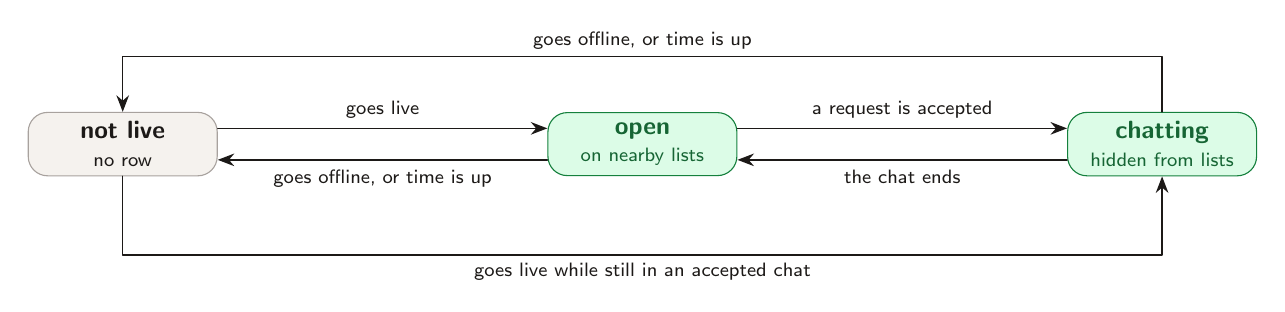
\begin{tikzpicture}
  \node[endstate, minimum width=24mm] (off) at (0,0) {not live\\[-1pt]{\scriptsize\mdseries no row}};
  \node[state, minimum width=24mm] (open) at (6.6,0) {open\\[-1pt]{\scriptsize\mdseries on nearby lists}};
  \node[state, minimum width=24mm] (chatting) at (13.2,0) {chatting\\[-1pt]{\scriptsize\mdseries hidden from lists}};

  \draw[transition] ($(off.east)+(0,0.2)$) -- node[translabel, above=2pt, fill=none] {goes live} ($(open.west)+(0,0.2)$);
  \draw[transition] ($(open.west)+(0,-0.2)$) -- node[translabel, below=2pt, fill=none] {goes offline, or time is up} ($(off.east)+(0,-0.2)$);
  \draw[transition] ($(open.east)+(0,0.2)$) -- node[translabel, above=2pt, fill=none] {a request is accepted} ($(chatting.west)+(0,0.2)$);
  \draw[transition] ($(chatting.west)+(0,-0.2)$) -- node[translabel, below=2pt, fill=none] {the chat ends} ($(open.east)+(0,-0.2)$);
  \draw[transition] (chatting.north) -- ++(0,0.7) -| node[translabel, pos=0.25, above=1pt, fill=none] {goes offline, or time is up} (off.north);
  \draw[transition] (off.south) -- ++(0,-1.0) -| node[translabel, pos=0.25, below=1pt, fill=none] {goes live while still in an accepted chat} (chatting.south);
\end{tikzpicture}

  \caption{Live state of one user. ``Not live'' means the user has no \code{availability} row. Any chat
    ending returns both users to \code{open} if they are still live.}
  \label{fig:live-states}
\end{figure}

\subsection{Requests and chats}

\code{chat_requests} records every say-hi request. A request names its sender (\code{from_user}) and
recipient (\code{to_user}), which must differ, and has a status. It expires five minutes after it is
created unless it is answered. When the recipient accepts, the same row becomes the chat: its ID is the
chat's ID, its status stays \code{accepted} while the chat lasts, and \code{ended_at} records when it
ended. \code{responded_at} records when the recipient answered. A partial unique index allows at most one
\code{pending} request per sender.

\Cref{fig:request-states} shows the lifecycle of the status column and \cref{tab:request-transitions}
lists every transition with the code that performs it.

\begin{figure}[ht]
  \centering
  % Lifecycle of a say-hi request: the status column of chat_requests (Figure: request states).
% Labels are short; the table of request transitions gives every trigger.
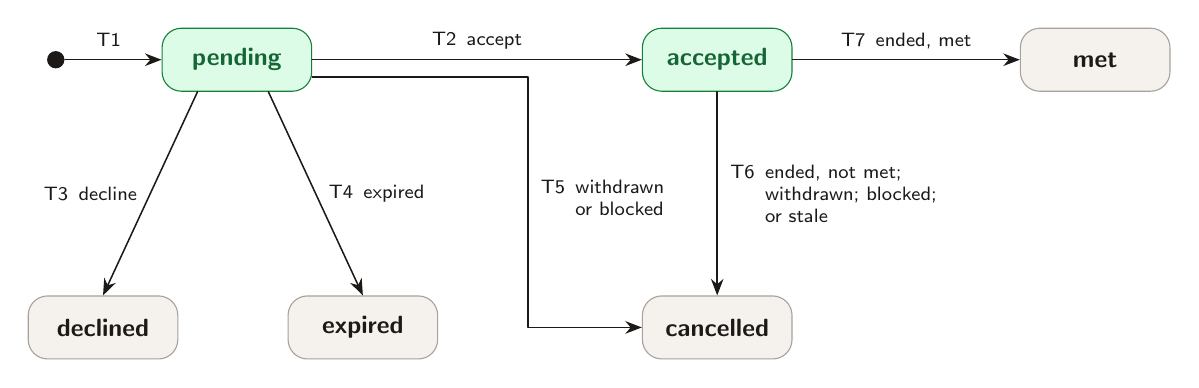
\begin{tikzpicture}
  \node[startdot] (start) at (0,0) {};
  \node[state] (pending) at (2.3,0) {pending};
  \node[state] (accepted) at (8.4,0) {accepted};
  \node[endstate] (met) at (13.2,0) {met};
  \node[endstate] (declined) at (0.6,-3.4) {declined};
  \node[endstate] (expired) at (3.9,-3.4) {expired};
  \node[endstate] (cancelled) at (8.4,-3.4) {cancelled};

  \draw[transition] (start) -- (pending);
  \node[translabel, fill=none, above=3pt] at ($(start)!0.5!(pending.west)$) {T1};
  \draw[transition] (pending) -- node[translabel, above=2pt, fill=none] {T2\enskip accept} (accepted);
  \draw[transition] (accepted) -- node[translabel, above=2pt, fill=none] {T7\enskip ended, met} (met);
  \draw[transition] ($(pending.south)+(-0.5,0)$) -- node[translabel, left=3pt, fill=none] {T3\enskip decline} (declined.north);
  \draw[transition] ($(pending.south)+(0.4,0)$) -- node[translabel, right=3pt, fill=none] {T4\enskip expired} (expired.north);
  \draw[transition] ($(pending.east)+(0,-0.22)$) -- (6.0,-0.22) |- (cancelled.west);
  \node[translabel, fill=none, align=left, anchor=west] at (6.1,-1.75) {T5\enskip withdrawn\\\hphantom{T5\enskip}or blocked};
  \draw[transition] (accepted.south) -- node[translabel, right=3pt, fill=none, align=left] {T6\enskip ended, not met;\\\hphantom{T6\enskip}withdrawn; blocked;\\\hphantom{T6\enskip}or stale} (cancelled.north);
\end{tikzpicture}

  \caption{Lifecycle of a request. Grey states are final. The labels refer to
    \cref{tab:request-transitions}.}
  \label{fig:request-states}
\end{figure}

\begin{table}[ht]
  \centering
  \caption{Request transitions.}
  \label{tab:request-transitions}
  \tablefont
  \begin{tabularx}{\textwidth}{@{}L{8mm}L{44mm}Y@{}}
    \toprule
    & \textsf{\textbf{Transition}} & \textsf{\textbf{Performed by}} \\
    \midrule
    T1 & created as \code{pending} & \code{send_request}, called by the sender \\
    T2 & \code{pending} to \code{accepted} & \code{respond} with \code{accept = true}, called by the recipient \\
    T3 & \code{pending} to \code{declined} & \code{respond} with \code{accept = false}, called by the recipient \\
    T4 & \code{pending} to \code{expired} & \code{expire_stale}, once five minutes have passed or the sender is no longer live; \code{send_request} also expires the sender's own request whose time is up before checking for one already waiting \\
    T5 & \code{pending} to \code{cancelled} & \code{cancel_request} (the sender withdraws it); \code{go_offline} (the sender goes offline); \code{respond} when the sender accepts someone else's request; \code{block_user} by either person \\
    T6 & \code{accepted} to \code{cancelled} & \code{end_chat} with outcome \code{cancelled}; \code{cancel_request} when the cancel arrives just after an accept; \code{block_user} by either person; \code{expire_stale} once neither person is live \\
    T7 & \code{accepted} to \code{met} & \code{end_chat} with outcome \code{met} \\
    \bottomrule
  \end{tabularx}
\end{table}

The sender never learns why a request did not lead to a chat. The client treats every final status other
than \code{accepted} as \ui{Not this time} (\cref{sec:flow-sayhi}).

\subsection{Messages}

\code{messages} holds the messages of both kinds of chat. A check constraint requires exactly one parent:
\code{request_id} for a one-to-one chat or \code{event_id} for an event's group chat. The body is 1 to
1000 characters. \code{sender_name} stores the sender's display name (first name and last initial) at the
time of sending, because a message delivered over Realtime must be renderable on its own: the recipient
cannot read the sender's profile row to look the name up.

\subsection{Events and members}

\code{events} holds the public events on the map. Each has a host, a category, a title (1 to 60
characters), a description (up to 200 characters), a position and a start time. The position is a place
the host chose on the map and is, by design, the one location in the system that other users are meant
to see. The \code{emoji} column stores the category as one of twelve emoji values; the client maps each
value to an icon and a name (\cref{tab:event-categories}). \code{event_members} records who has joined
which event. The host is added as a member when the event is created, and only the host can delete the
event (\code{delete_event}); its members and messages are deleted with it.

\subsection{Blocks and reports}

\code{blocks} records that one user has blocked another; the pair is the primary key and a user cannot
block themselves. Although each row has a direction, the server applies a block in both directions
(\cref{sec:blocking-reporting}). \code{reports} records a report: who reported whom, an optional request
the report relates to, one of six reasons (\code{inappropriate-photo}, \code{harassment}, \code{unsafe},
\code{spam-or-fake}, \code{under-18}, \code{other}) and up to 500 characters of details. The columns
\code{reviewed_at} and \code{action} exist for a later human review; nothing in the repository writes
them.

\subsection{Location changes}

\code{private.location_changes} records the time at which each user started a live session or moved more
than 150 metres while live. It stores no position. \code{go_green} counts the rows from the last ten
minutes to limit how often a location may change, and the minute job deletes rows older than that
(\cref{sec:relocation-limits}).

\subsection{Event posts}

\code{private.event_posts} records the time each event was created, and nothing else. \code{create_event}
counts the rows from the last 24 hours for its five-a-day limit, so deleting an event does not give its
place back; the minute job deletes rows older than a day.

\subsection{Photos in Storage}

Photo files are objects in the Storage bucket \code{photos}, which is private, accepts JPEG, PNG and
WebP, and limits each file to 5\,MiB. The app names every object
\code{<user-id>/<slot>-<milliseconds>.jpg}, where the slot is \code{profile} for the profile picture and
\code{photo0} to \code{photo5} for the others. The profile picture also has a 320-pixel copy at the same
path with the suffix \code{-small.jpg}, used for small avatars.

\section{Indexes}

\Cref{tab:indexes} lists the indexes beyond the primary keys and what each one serves.

\begin{table}[ht]
  \centering
  \caption{Secondary indexes.}
  \label{tab:indexes}
  \tablefont
  \begin{tabularx}{\textwidth}{@{}L{78mm}Y@{}}
    \toprule
    \textsf{\textbf{Index}} & \textsf{\textbf{Serves}} \\
    \midrule
    \code{availability (location)}, GiST & Distance queries in \code{nearby} and \code{near_each_other} \\
    \code{availability (expires_at)} & The minute job's deletion of ended sessions \\
    \code{chat_requests (from_user)} where \code{pending}, unique & At most one waiting request per sender \\
    \code{chat_requests (to_user)} & Looking up a recipient's waiting requests \\
    \code{chat_requests (from_user, created_at)} & The rate limit on sending requests \\
    \code{chat_requests (expires_at)} where \code{pending} & Expiring unanswered requests \\
    \code{chat_requests (from_user, to_user)} where \code{accepted} & One-chat checks, \code{my_status} and stale-chat cleanup \\
    \code{events (location)}, GiST & Radius queries in \code{events_near} \\
    \code{events (host)}, \code{events (starts_at)} & Rate limit on creating events; time filter \\
    \code{event_members (user_id)} & Membership lookups by user \\
    \code{messages (request_id, created_at)} & One-to-one chat history \\
    \code{messages (event_id, created_at)} & Group chat history \\
    \code{messages (sender, created_at)} & The rate limit on sending messages \\
    \code{blocks (blocked)} & Block checks in the reverse direction \\
    \code{reports (reported)}, \code{(reporter)}, \code{(request_id)} & Counting reporters; cascades \\
    \code{private.location_changes (user_id, changed_at)} & The relocation limit in \code{go_green} \\
    \code{private.event_posts (user_id, posted_at)} & The event limit in \code{create_event} \\
    \bottomrule
  \end{tabularx}
\end{table}

\section{Data the client works with}
\label{sec:client-types}

The client does not mirror the tables. It works with a small set of shapes defined in
\code{src/data/types.ts}, built by the API layer from what the server returns (\cref{tab:client-types}).

\begin{table}[ht]
  \centering
  \caption{Client data shapes and their sources.}
  \label{tab:client-types}
  \tablefont
  \begin{tabularx}{\textwidth}{@{}L{32mm}L{48mm}Y@{}}
    \toprule
    \textsf{\textbf{Type}} & \textsf{\textbf{Built from}} & \textsf{\textbf{Holds}} \\
    \midrule
    \code{Profile} & the user's own \code{profiles} row & All profile fields, with photos as signed URLs \\
    \code{NearbyPerson} & a person card & What another user may see; photo URLs signed on demand \\
    \code{Availability} & \code{go_green} or \code{my_status} & Duration, note, server start and end times \\
    \code{OutgoingRequest} & \code{send_request} or \code{my_status} & Request ID, recipient, end time, status \code{pending}, \code{accepted} or \code{not-this-time} \\
    \code{IncomingRequest} & a Realtime insert or a query, then \code{request_person} & Request ID, sender's card, end time \\
    \code{ChatSession} & an accepted request & Chat ID, partner, status \code{active} or \code{other-cancelled}, messages \\
    \code{Message} & a \code{messages} row & ID, sender (\code{me} for one's own), sender name, text, time \\
    \code{MapEvent} & an event card & Event fields, host name and photo, member count, joined flag, loaded messages \\
    \bottomrule
  \end{tabularx}
\end{table}

\subsection{The person card}
\label{sec:person-card}

A \term{person card} is the only form in which one user's profile reaches another user. The helper
\code{private.person_card(target)} builds it as JSON with these fields: ID, first name, last initial,
gender (only if the owner chose to show it and did not choose \code{prefer-not}), introduction,
interests, the storage paths of the profile picture and other photos, the live note, and the
\code{verified} flag. It contains no last name, no location and no distance. Every function that returns
a full profile (\code{nearby}, \code{request_person}, \code{my_status}) returns person cards, so this helper
is the single definition of what a profile reveals. Two places return less: \code{blocked_list} returns
only ID, first name and last initial, and an event card's host adds only the profile picture's path to
those.

\subsection{Event categories}

The category of an event is stored as an emoji value in \code{events.emoji}. The app shows an icon and a
name instead; the table \code{EVENT_CATEGORIES} in \code{src/data/constants.ts} maps one to the other
(\cref{tab:event-categories}). A value missing from the table, for example one written by a newer app,
falls back to a calendar icon named \ui{Event}. The database default is the first value, Coffee.

\begin{table}[ht]
  \centering
  \caption{Event categories. Stored values are given as Unicode code points.}
  \label{tab:event-categories}
  \tablefont
  \begin{tabular}{@{}lll@{\hspace{12mm}}lll@{}}
    \toprule
    \textsf{\textbf{Name}} & \textsf{\textbf{Icon}} & \textsf{\textbf{Value}} & \textsf{\textbf{Name}} & \textsf{\textbf{Icon}} & \textsf{\textbf{Value}} \\
    \midrule
    Coffee & \code{cafe} & U+2615 & Sports & \code{basketball} & U+1F3C0 \\
    Food & \code{pizza} & U+1F355 & Music & \code{musical-notes} & U+1F3B8 \\
    Games & \code{dice} & U+1F3B2 & Walk & \code{walk} & U+1F6B6 \\
    Study & \code{library} & U+1F4DA & Yoga & \code{flower} & U+1F9D8 \\
    Coding & \code{laptop} & U+1F4BB & Movies & \code{film} & U+1F3AC \\
    Art & \code{color-palette} & U+1F3A8 & Drinks & \code{beer} & U+1F37B \\
    \bottomrule
  \end{tabular}
\end{table}

\chapter{Server interface}
\label{ch:server-interface}

The client reaches the database in two ways: by calling database functions and by reading the few tables
it is allowed to read. \Cref{fig:call-anatomy} follows one function call from the store to the tables and
back. This chapter is the reference for the interface; \cref{app:db-functions,app:tables} give the exact
signatures and table definitions.

\begin{figure}[ht]
  \centering
  % Anatomy of a database function call, with send_request as the example (Figure: call anatomy).
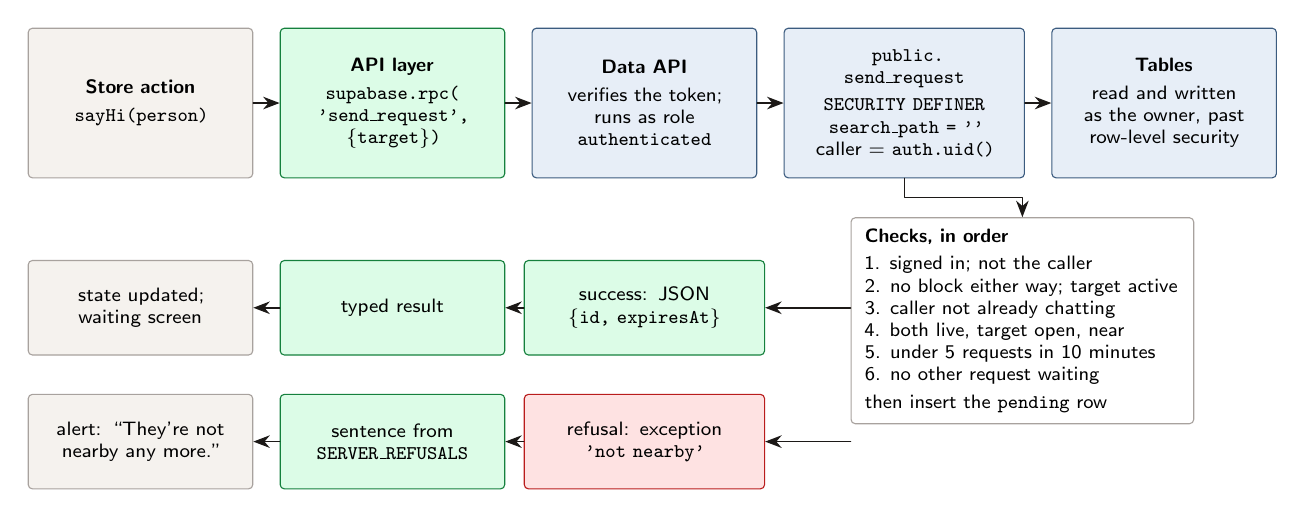
\begin{tikzpicture}[
    stage/.style={box, font=\sffamily\scriptsize, text width=25mm, minimum height=19mm, align=center},
    lab/.style={font=\sffamily\scriptsize, text=muted, inner sep=1.2pt, align=center},
  ]
  \node[stage, clientbox] (store) at (1.45,0) {\textbf{Store action}\\[2pt]\texttt{sayHi(person)}};
  \node[stage, accentbox] (api) at (4.65,0) {\textbf{API layer}\\[2pt]\texttt{supabase.rpc(}\\\texttt{'send\_request',}\\\texttt{\{target\})}};
  \node[stage, serverbox] (rest) at (7.85,0) {\textbf{Data API}\\[2pt]verifies the token;\\runs as role\\\texttt{authenticated}};
  \node[stage, serverbox, text width=27mm] (fn) at (11.15,0) {\textbf{\texttt{public.}}\\\textbf{\texttt{send\_request}}\\[2pt]\texttt{SECURITY DEFINER}\\\texttt{search\_path = ''}\\caller = \texttt{auth.uid()}};
  \node[stage, serverbox] (tables) at (14.45,0) {\textbf{Tables}\\[2pt]read and written as the owner, past row-level security};

  \draw[flow] (store) -- (api);
  \draw[flow] (api) -- (rest);
  \draw[flow] (rest) -- (fn);
  \draw[flow] (fn) -- (tables);

  \node[box, font=\sffamily\scriptsize, text width=40mm, align=flush left, anchor=north] (checks) at (12.65,-1.45)
    {\textbf{Checks, in order}\\[2pt]
     1. signed in; not the caller\\
     2. no block either way; target active\\
     3. caller not already chatting\\
     4. both live, target open, near\\
     5. under 5 requests in 10 minutes\\
     6. no other request waiting\\[2pt]
     then insert the \texttt{pending} row};
  \draw[flow] (fn.south) |- ($(checks.north)+(0,0.25)$) -- (checks.north);

  \node[stage, minimum height=12mm, text width=27mm, accentbox] (ok) at (7.85,-2.6) {success: JSON\\\texttt{\{id, expiresAt\}}};
  \node[stage, minimum height=12mm, text width=27mm, draw=alert, fill=alertsoft] (no) at (7.85,-4.3) {refusal: exception\\\texttt{'not nearby'}};
  \draw[flow] (checks.west |- ok) -- (ok);
  \draw[flow] (checks.west |- no) -- (no);
  \node[stage, minimum height=12mm, accentbox] (convert) at (4.65,-2.6) {typed result};
  \node[stage, minimum height=12mm, accentbox] (sentence) at (4.65,-4.3) {sentence from\\\texttt{SERVER\_REFUSALS}};
  \draw[flow] (ok) -- (convert);
  \draw[flow] (no) -- (sentence);
  \node[stage, minimum height=12mm, clientbox] (stateset) at (1.45,-2.6) {state updated;\\waiting screen};
  \node[stage, minimum height=12mm, clientbox] (alert) at (1.45,-4.3) {alert: ``They're not\\nearby any more.''};
  \draw[flow] (convert) -- (stateset);
  \draw[flow] (sentence) -- (alert);
\end{tikzpicture}

  \caption{Anatomy of a database function call, with \code{send_request} as the example. The function
    runs as its owner, takes the caller's identity from the token, and either writes after its checks or
    raises a short refusal that the API layer turns into a sentence.}
  \label{fig:call-anatomy}
\end{figure}

\section{Conventions}
\label{sec:function-conventions}

All database functions follow the same conventions, set out at the top of the migration that defines
them.

\begin{itemize}
  \item Functions in \code{public} are the API. They are declared \code{SECURITY DEFINER}, so they run
    as their owner and are not limited by row-level security, and \code{SET search_path = ''}, so every
    name inside them is schema-qualified and cannot be redirected by the caller.
  \item The caller is always \code{auth.uid()}, read from the session token. No function takes a user ID
    that it trusts as the caller's identity.
  \item Execution is revoked from the roles \code{public} and \code{anon}, so only a signed-in user
    (role \code{authenticated}) can call them. Helpers in \code{private} cannot be called through the
    Data API at all, because that schema is not exposed.
  \item A function refuses a request by raising an exception with a short, fixed message, for example
    \code{not nearby} or \code{too many requests}. The client translates each message into a sentence
    (\cref{app:refusals}).
  \item Functions that return a full profile return person cards (\cref{sec:person-card});
    \code{blocked_list} and an event card's host return a reduced object with no introduction, interests
    or note. Functions that return events return event cards. Both are JSON objects with camel-case keys
    that match the client's types, and the instants in them are milliseconds since the Unix epoch. The
    two message functions are the exception: they return the stored \code{messages} row, whose
    \texttt{created\_at} is an ISO~8601 string.
\end{itemize}

\section{Database functions}
\label{sec:functions}

\Cref{tab:functions} lists every function the client calls, in the order of the user's journey. The
\emph{Checks} column lists what the function verifies before it changes anything, with the refusal
message in parentheses where one applies.

\begingroup\tablefont
\begin{longtable}{@{}L{38mm}L{\dimexpr\linewidth-38mm-2\tabcolsep\relax}@{}}
  \caption{Database functions called by the client.}
  \label{tab:functions}\\
  \toprule
  \textsf{\textbf{Function}} & \textsf{\textbf{Effect and checks}} \\
  \midrule
  \endfirsthead
  \toprule
  \textsf{\textbf{Function}} & \textsf{\textbf{Effect and checks}} \\
  \midrule
  \endhead
  \bottomrule
  \endfoot
  \multicolumn{2}{@{}l}{\textsf{\textbf{Going live}}} \\[2pt]
  \code{go_green}\newline{\scriptsize lat, lng, accuracy, minutes, note}\newline{\scriptsize returns start and end times}
  & Starts or updates the caller's live session and returns its server times.
    Checks: signed in (\code{not signed in}); profile finished and adult (\code{profile not ready}) and
    active (\code{account restricted}); duration is 30, 60 or 120 (\code{invalid duration}); note of
    at most 60 characters (\code{note too long}); latitude and longitude in range (\code{invalid location}).
    Applies the relocation rules of \cref{sec:relocation-limits} under a per-user lock: a move of 150\,m
    or less keeps the stored position and start time; a larger move while live must not exceed 150\,m plus
    10\,km/h over the time since the position was set (\code{moving too fast}); going live when not live
    must be within 5\,km plus 1000\,km/h of the last known position (\code{location jumped}); and at most
    three location changes are allowed in ten minutes, shared with \code{set_map_position} (\code{too many
    location changes}). Stores the centre of the position's cell, the accuracy clamped to 0--50\,m, and the
    session as \code{chatting} if the caller has an accepted chat, otherwise \code{open}, ending
    \code{minutes} after now. The stored position also becomes the caller's last known position. \\
  \code{update_note}\newline{\scriptsize note}
  & Replaces the live note. Checks: an active profile, as for \code{go_green}; at most 60 characters
    (\code{note too long}). Does nothing if the caller is not live. \\
  \code{go_offline}
  & Withdraws the caller's waiting request (status \code{cancelled}), then deletes the caller's live
    session. Always succeeds. \\
  \code{nearby}\newline{\scriptsize returns person cards}
  & Returns up to 50 person cards of users who are live, \code{open}, not expired and active, in the
    caller's cell or a touching one (\cref{sec:location-privacy}), excluding the caller and anyone blocked
    in either direction. Returns nothing if the caller is not live. Never returns a position or a
    distance. At most 12 calls a minute (\code{too many lookups}). \\[3pt]
  \multicolumn{2}{@{}l}{\textsf{\textbf{Say hi and chat}}} \\[2pt]
  \code{send_request}\newline{\scriptsize target}\newline{\scriptsize returns ID and end time}
  & Creates a request to \code{target} that expires in five minutes. Checks, in order: signed in, with an
    active profile (\code{account restricted}); not the caller (\code{cannot request yourself}); no block either way and target active (\code{not available}).
    If the caller is already waiting on this same person, it returns that request instead, so a second tap
    sends nothing new. Then: caller not already in a chat (\code{already chatting}); target live, \code{open} and near the caller,
    who must also be live (\code{not nearby}); fewer than five requests sent in ten minutes
    (\code{too many requests}). It then marks the caller's own timed-out request as expired and refuses if
    one is still waiting (\code{already waiting}). The partial unique index enforces the same rule if two
    calls race. \\
  \code{cancel_request}\newline{\scriptsize request\_id}
  & The sender withdraws a request. Locks the caller's request if it is \code{pending} or
    \code{accepted} and sets it to \code{cancelled}; if it had just been accepted, it also returns both
    users to \code{open}. Returns silently if there is nothing left to cancel. \\
  \code{respond}\newline{\scriptsize request\_id, accept}
  & The recipient answers. Locks the request, which must be \code{pending} and addressed to the caller
    (\code{no such pending request}) and not past its end time (\code{request expired}). A decline sets
    \code{declined}. An accept requires the sender to be live (\code{not available}), withdraws the
    caller's own waiting request, refuses if the caller (\code{already chatting}) or the sender
    (\code{not available}) is already in a chat, then sets \code{accepted} and sets both users to
    \code{chatting}. \\
  \code{request_person}\newline{\scriptsize request\_id}\newline{\scriptsize returns a person card}
  & Returns the other participant's card, or nothing. Nothing if either user has blocked the other or either is not active. The
    recipient may see the sender's card at any stage; the sender may see the recipient's card only once
    the request was accepted (status \code{accepted} or \code{met}, or \code{cancelled} after an accept).
    The live note is removed once the request or chat is over. \\
  \code{end_chat}\newline{\scriptsize request\_id, outcome}
  & Ends the caller's accepted chat with outcome \code{met} or \code{cancelled} (\code{invalid outcome}
    otherwise; \code{no such chat} if it is not an accepted chat of the caller) and returns both users to
    \code{open}. \\
  \code{send_chat_message}\newline{\scriptsize request\_id, body}\newline{\scriptsize returns the message}
  & Checks: an active profile (\code{account restricted}); body of 1 to 1000 characters (\code{invalid
    message}); an accepted chat of the caller (\code{no such chat}); no block between the two (\code{not available}); fewer than 30 messages sent by
    the caller in the last minute (\code{too many messages}). Stores the message with the sender's display
    name and returns the saved row. \\
  \code{my_status}\newline{\scriptsize returns live, chat and request}
  & What the app needs after a restart: the caller's live session (note, start and end) if not expired;
    the ID of the caller's newest accepted chat in which at least one person is still live; and the
    caller's waiting request with the recipient's card, if one has not expired. Also returns the server's
    clock (\texttt{now}, in milliseconds), which the app uses to correct for a phone whose clock is wrong
    (\cref{sec:time}). \\[3pt]
  \multicolumn{2}{@{}l}{\textsf{\textbf{Safety and account}}} \\[2pt]
  \code{block_user}\newline{\scriptsize target}
  & Records the block (repeating it is harmless). Checks: signed in; not the caller
    (\code{cannot block yourself}). Cancels any accepted chat and any waiting request between the two; if
    it ended a chat, returns both users to \code{open}. A chat either user has with someone else is not
    affected. \\
  \code{blocked_list}\newline{\scriptsize returns names}
  & The caller's blocked users, newest first, as ID, first name and last initial. \\
  \code{report_user}\newline{\scriptsize target, reason, details, request\_id}
  & Reports a person. Saves a copy of their profile (name, intro, interests, live note, photo paths)
    in the report's \code{content}, and, when the request is a say-hi or chat between the two users, the
    last 20 messages the reported person sent in it; any other request is dropped. Then files the report
    through \code{private.file_report}, which every report goes through. Its checks: signed in; not the
    caller (\code{cannot report yourself}); the target exists (\code{not available}); the reason is one of
    the six values (\code{invalid reason}); the details are at most 500 characters of clean text
    (\code{invalid details}). A second report of the same thing (the same person, message or event)
    within a day returns without a new row, so a double tap files one report; otherwise fewer than ten
    reports by the caller in 24 hours (\code{too many reports}). Records whether the report counts towards
    the automatic hide (\cref{sec:blocking-reporting}). Sets the reported profile to \code{hidden}, and
    ends everything the person is in, once three different users' counted reports that are not yet
    reviewed name it; a per-person lock makes reports sent at once still count. \\
  \code{report_message}\newline{\scriptsize message\_id, reason, details}
  & Reports one group-chat message. Refused (\code{content not available}) unless the message exists
    and the caller is in its event. Files a report about its sender through \code{private.file_report},
    with \code{message_id}, \code{event_id} and a copy of the body, send time and event title. \\
  \code{report_event}\newline{\scriptsize event\_id, reason, details}
  & Reports an event. Refused (\code{content not available}) unless the caller joined it or the map would
    list it for them (not blocked, started at most 3 hours ago, within 50\,km of the position the server
    holds). Files a report about its host through \code{private.file_report}, with \code{event_id} and a
    copy of the emoji, title, description, start and creation times. \\
  \code{delete_account}
  & Refuses (\code{photos not removed}) while any file is left in the caller's photo folder. The client
    removes every file there through the Storage API before calling it. Returns the caller's chat partner,
    if any, to \code{open}, deletes any ban on the caller's email address, their upload times and their
    Auth sign-in flows and audit records, then deletes the caller's Auth user, which cascades through every
    table except \code{reports}, where the caller's id becomes null (\cref{sec:flow-delete}). \\[3pt]
  \multicolumn{2}{@{}l}{\textsf{\textbf{Map events}}} \\[2pt]
  \code{set_map_position}\newline{\scriptsize lat, lng}
  & Stores the centre of the position's cell as the caller's last known position, which the map uses for
    two hours. Checks: an active profile; latitude and longitude in range (\code{invalid location}). Applies
    the relocation rules under the same per-user lock as \code{go_green}: a move of 150\,m or less from the
    last known position keeps it and renews its time; a larger move must be within 5\,km plus 1000\,km/h
    over the time since the last known position was set, however long ago (\code{location jumped}); and a
    change counts towards the three in ten minutes (\code{too many location changes}) unless the caller's
    live position is already there. \\
  \code{events_near}\newline{\scriptsize radius\_m}\newline{\scriptsize returns event cards}
  & Returns up to 50 event cards within \code{radius_m} (default 10\,km, never more than 50\,km) of the
    position the server holds for the caller: the last position \code{set_map_position} or \code{go_green}
    stored, if set in the last two hours (\code{location needed} otherwise). Only events that started less than three hours ago or
    have not started, whose host is active and not blocked in either direction, ordered by start time.
    At most 20 calls a minute (\code{too many lookups}). \\
  \code{create_event}\newline{\scriptsize emoji, title, description, lat, lng, starts\_at\_ms}\newline{\scriptsize returns an event card}
  & Creates an event and adds the host as its first member. Checks: signed in; profile finished and adult
    (\code{profile not ready}) and active (\code{account restricted}); valid position (\code{invalid location}); a title of 1 to 60 characters on
    one line with something visible (\code{invalid title}); details of at most 200 characters of clean text
    (\code{invalid details}); start between five minutes ago and seven days ahead, checked before the
    number is converted (\code{invalid start time}); fewer than five events created by the caller in 24
    hours, counting events since deleted (\code{too many events}). Each creation is recorded in
    \code{private.event_posts}. The category must be one of the app's twelve (check constraint
    \code{events_emoji_category}). \\
  \code{join_event}\newline{\scriptsize event\_id}
  & Adds the caller as a member (repeating it is harmless). Checks: signed in; the event exists
    (\code{no such event}); no block between the caller and the host (\code{not available}); an active
    profile; a position the server holds for the caller, as for \code{events_near} (\code{location
    needed}), within 5\,km of the event (\code{too far away}). The app sends the phone's position to
    \code{set_map_position} first. \\
  \code{delete_event}\newline{\scriptsize event\_id}
  & Deletes the event; its members and group-chat messages go with it through cascading foreign keys.
    Checks: signed in; the event exists (\code{no such event}); the caller is its host (\code{not the host}). \\
  \code{leave_event}\newline{\scriptsize event\_id}
  & If the caller hosts the event, deletes it with its members and messages; otherwise removes the
    caller's membership. \\
  \code{send_event_message}\newline{\scriptsize event\_id, body}\newline{\scriptsize returns the message}
  & Checks: an active profile (\code{account restricted}); body of 1 to 1000 characters (\code{invalid
    message}); the caller is a member (\code{not a member}); fewer than 30 messages in the last minute (\code{too many messages}). Stores
    the message with the sender's display name and returns the saved row. \\
\end{longtable}
\endgroup

\Cref{tab:crud} shows which tables each function reads and writes. It is the quickest way to find every
function that can change a given table.

\begin{table}[ht]
  \centering
  \caption[Table access by function]{Table access by function: R read, I insert, U update, D delete. Columns: \code{profiles},
    \code{availability}, \code{chat_requests}, \code{messages}, \code{events}, \code{event_members},
    \code{blocks}, \code{reports}, \code{private.location_changes}.}
  \label{tab:crud}
  \tablefont
  \newcommand{\h}[1]{\rotatebox{90}{\code{#1}}}
  \setlength{\tabcolsep}{3pt}
  \begin{tabular}{@{}l*{9}{>{\centering\arraybackslash}p{8.5mm}}@{}}
    \toprule
    & \h{profiles} & \h{availability} & \h{chat_requests} & \h{messages} & \h{events} & \h{event_members} & \h{blocks} & \h{reports} & \h{location_changes} \\
    \midrule
    \code{go_green} & R & RIU & R & & & & & & RI \\
    \code{set_map_position} & R & R & & & & & & & RI \\
    \code{update_note} & R & U & & & & & & & \\
    \code{go_offline} & & D & U & & & & & & \\
    \code{nearby} & R & R & & & & & R & & \\
    \code{send_request} & R & R & RIU & & & & R & & \\
    \code{cancel_request} & & U & RU & & & & & & \\
    \code{respond} & & RU & RU & & & & & & \\
    \code{request_person} & R & R & R & & & & R & & \\
    \code{end_chat} & & U & RU & & & & & & \\
    \code{send_chat_message} & R & & R & RI & & & R & & \\
    \code{my_status} & R & R & R & & & & & & \\
    \code{block_user} & & U & U & & & & I & & \\
    \code{blocked_list} & R & & & & & & R & & \\
    \code{report_user} & RU & RUD & RU & R & & RD & & RI & \\
    \code{report_message} & RU & UD & RU & R & R & RD & & RI & \\
    \code{report_event} & RU & UD & RU & R & R & RD & R & RI & \\
    \code{delete_account} & RD\textsuperscript{*} & U & R & & & & & U & \\
    \code{events_near} & R & R & & & R & R & R & & \\
    \code{create_event} & R & & & & RI & RI & & & \\
    \code{join_event} & R & R & & & R & I & R & & \\
    \code{leave_event} & & & & & RD & D & & & \\
    \code{delete_event} & & & & D\textsuperscript{\dag} & RD & D\textsuperscript{\dag} & & & \\
    \code{send_event_message} & R & & & RI & & R & & & \\
    \code{expire_stale} (job) & & RD & RU & & & & & & D \\
    \midrule
    Client, directly & RIU & & R & R & & & D & & \\
    \bottomrule
  \end{tabular}
  \par\smallskip\raggedright\footnotesize\textsuperscript{*}\,\code{delete_account} deletes the
  \code{auth.users} row; the cascade removes the profile and every row that references it, and sets
  the user's id to null in \code{reports}. Before that it deletes the user's rows in
  \code{private.banned_identities} and \code{private.photo_uploads}, which have no foreign key.
  \textsuperscript{\dag}\,By cascade from the deleted event; \code{leave_event} by its host deletes in the same way.
  Not shown: \code{create_event} also inserts into \code{private.event_posts}; \code{set_map_position}
  and \code{go_green} write \code{private.last_positions}, which they, \code{events_near} and
  \code{join_event} read; and \code{nearby} and \code{events_near} count calls in
  \code{private.call_counts}. The minute job prunes the event posts and call counts.
\end{table}

Two details of these functions carry more weight than their size suggests. First, \code{respond},
\code{cancel_request} and \code{end_chat} lock the request row with \code{SELECT \dots FOR UPDATE} before
deciding, so a cancel and an accept that arrive together are applied one after the other, and the second
sees the first one's result. Second, \code{respond} withdraws the caller's own waiting request
\emph{before} it checks whether the caller is already chatting. If an answer to that request is being
committed at the same moment, the update waits for it, and the check that follows sees the result.

\section{Direct table access}
\label{sec:direct-access}

The client reads and writes a few tables directly through the Data API, always within the limits of
row-level security and column grants (\cref{tab:direct-access}).

\begin{table}[ht]
  \centering
  \caption{Direct table and storage access by the client.}
  \label{tab:direct-access}
  \tablefont
  \begin{tabularx}{\textwidth}{@{}L{30mm}L{40mm}Y@{}}
    \toprule
    \textsf{\textbf{Table}} & \textsf{\textbf{Operation}} & \textsf{\textbf{Used for}} \\
    \midrule
    \code{profiles} & select, insert, update own row & Loading and saving the user's own profile (\code{fetchMyProfile}, \code{saveProfile}) \\
    \code{chat_requests} & select rows the user takes part in & Missed incoming requests (\code{pendingIncoming}), the status of a request or chat (\code{requestStatus}), the answer poll in \code{waitForAnswer} \\
    \code{messages} & select & Chat and group chat history, newest 200 (\code{fetchMessages}) \\
    \code{blocks} & delete own row & Unblocking (\code{unblock}) \\
    \code{storage.objects} & upload, list, remove, sign & Photos in the user's own folder; signed URLs for photos the user may see \\
    \bottomrule
  \end{tabularx}
\end{table}

A profile row is inserted the first time it is saved and updated after that, never upserted. An upsert
would also try to set \code{id} and \code{is_adult} on conflict, and the column grants allow a client to
update only the editable columns, so the database would refuse it.

\section{Private helpers}
\label{sec:helpers}

The functions share a small set of helpers in the \code{private} schema (\cref{tab:helpers}). Those
used by a row-level security policy, a storage policy or a check constraint must be executable by
signed-in users, because the policy or constraint runs them as the user. Each answers only for the
caller, or reads no tables at all.

\begingroup\tablefont
\begin{longtable}{@{}L{42mm}L{\dimexpr\linewidth-42mm-2\tabcolsep\relax}@{}}
  \caption{Private helpers.}
  \label{tab:helpers}\\
  \toprule
  \textsf{\textbf{Helper}} & \textsf{\textbf{Purpose}} \\
  \midrule
  \endfirsthead
  \toprule
  \textsf{\textbf{Helper}} & \textsf{\textbf{Purpose}} \\
  \midrule
  \endhead
  \bottomrule
  \endfoot
  \code{blocked_between(a, b)} & True if either user has blocked the other \\
  \code{person_card(target)} & The JSON card that is all another user may see of a profile \\
  \code{near_each_other(a, b)} & True if both users are live and their cell centres are at most 150\,m apart: the same cell or a touching one \\
  \code{cell_center(lat, lng)} & The centre of the cell of about 100\,m a position falls in; the only position ever stored \\
  \code{my_position(user)} & The position the server holds for a user: the last position from the map or going live, if set in the last two hours \\
  \code{require_active(user)} & Refuses with \code{not signed in}, \code{profile not ready} or \code{account restricted} unless the user has an active adult profile \\
  \code{count_call(user, list, max, per)} & Counts a call to \code{nearby} or \code{events_near} in a fixed window and refuses past the limit (\code{too many lookups}) \\
  \code{event_card(event, viewer)} & An event's fields, host name, member count and whether the viewer has joined; the host's photo path only when the viewer has joined \\
  \code{is_chat_participant(request)} & Used by the \code{messages} select policy; executable by signed-in users \\
  \code{is_event_member(event)} & Used by the \code{messages} select policy; executable by signed-in users \\
  \code{in_own_folder(paths, owner)} & Used by the photo check constraints; reads no tables \\
  \code{has_visible_text(value)} & True if the text shows at least one character, not only spaces, line breaks or invisible characters; used by check constraints and \code{create_event}; reads no tables \\
  \code{is_clean_text(value, multiline)} & True if the text has no control characters, direction overrides or more than three stacked accents, and no line breaks unless \code{multiline}; used the same way \\
  \code{valid_interests(interests)} & True for 3 to 5 different one-line interests of 1 to 30 characters in a plain list; used by a check constraint \\
  \code{my_photo_count()} & How many files the caller has in the \code{photos} bucket; used by the storage insert policy, which cannot read \code{storage.objects} itself \\
  \code{my_uploads_today()} & How many photos the caller uploaded in the last day; used by the storage insert policy \\
  \code{record_photo_upload()} & Trigger on \code{storage.objects}: records each upload to the \code{photos} bucket in \code{private.photo_uploads} \\
  \code{can_see_photo(object name)} & Used by the storage read policy (\cref{sec:photo-privacy}); executable by signed-in users \\
  \code{has_blocked_word(input)} & True if the text contains a word from \code{private.blocked_words} (\cref{sec:word-filter}) \\
  \code{refuse_blocked_words()} & The word-filter trigger function: refuses the row when a named column has a listed word \\
  \code{end_activity(user)} & Ends a user's live session, requests, chats and event memberships; used by the automatic hide and \code{suspend_user} \\
  \code{normalised_email(email)}, \code{email_hash(email)} & An address as the ban list compares it (lowercase, no \code{+tag}, no dots for Gmail), and its SHA-256 \\
  \code{ban_email_of(user, reason)} & Puts a user's email address on \code{private.banned_identities} \\
  \code{set_reported_hash()} & Trigger on \code{reports}: stores a hash of the reported id, which outlives the account \\
  \code{expire_stale()} & The minute job (\cref{sec:housekeeping}) \\
\end{longtable}
\endgroup

The definition of \emph{near} is worth quoting, because it decides who appears in a nearby list, who can
be sent a request and whose photos a user may load:

\begin{lstlisting}[language=pgsql, caption={The proximity test in \code{private.near_each_other}.}, label={lst:near}]
select exists (
  select 1
  from public.availability av_a
  join public.availability av_b on av_b.user_id = b
  where av_a.user_id = a
    and av_a.expires_at > now()
    and av_b.expires_at > now()
    and extensions.st_dwithin(av_a.location, av_b.location, 150)
);
\end{lstlisting}

Both stored positions are cell centres, so the test asks whether the two users are in the same cell of
about 100 metres or a touching one. The distance is fixed and the same for everyone; nothing the caller
sends changes it (\cref{sec:location-privacy}). Distances are computed on the geography type, in metres
on the Earth's surface.

\section{Word filter}
\label{sec:word-filter}

The app stores require a filter for objectionable content in an app where people post text and meet.
Yap's filter is a short list of words in \code{private.blocked_words}, checked by triggers before a row is
saved (\cref{tab:word-filter}). A row that contains a listed word is refused with \code{objectionable
text}, which the app shows as \ui{That has words Yap doesn't allow (see the community guidelines). Change
them and try again.} Because the check runs on the tables, it covers the profile, which the client writes
directly, as well as the database functions that save a note, an event or a message.

\begin{table}[ht]
  \centering
  \caption{Text checked by the word filter.}
  \label{tab:word-filter}
  \tablefont
  \begin{tabularx}{\textwidth}{@{}L{34mm}L{44mm}Y@{}}
    \toprule
    \textsf{\textbf{Trigger}} & \textsf{\textbf{Columns}} & \textsf{\textbf{Written by}} \\
    \midrule
    \code{profiles_word_filter} & \code{intro}, \code{interests} & The client's own profile saves \\
    \code{availability_word_filter} & \code{note} & \code{go_green}, \code{update_note} \\
    \code{events_word_filter} & \code{title}, \code{description} & \code{create_event} \\
    \code{messages_word_filter} & \code{body} & \code{send_chat_message}, \code{send_event_message} \\
    \bottomrule
  \end{tabularx}
\end{table}

\code{private.has_blocked_word} lowercases the text, splits it into words at every character that is not a
letter or digit, and compares each word with the list exactly. It repeats the comparison once with common
look-alike characters swapped back (\code{0} to \code{o}, \code{1} to \code{i}, \code{3} to \code{e},
\code{4} to \code{a}, \code{5} to \code{s}, \code{7} to \code{t}, \code{@} to \code{a}, \texttt{\$} to
\code{s}), so \code{h4te} is checked as \code{hate}. Only whole words match, so a longer word that merely
contains a listed one is never refused. Interests, a text array, are checked as their JSON text, which
splits the same way.

Names are not checked, because a real name can match a listed word, and report details are not checked,
so people can quote what was said to them. The list is deliberately narrow: it leaves out general
swearing, sexual words, words people use to describe harm or ask for help, and words that are also names
or ordinary words. It is a first line only; reports and blocks handle everything else. Rows saved before
the filter existed are not checked again; only new text and edits are.

\section{Moderation function}
\label{sec:moderation}

\code{private.suspend_user(target, note)} acts on a report after the owner has reviewed it. It is run from
the Supabase SQL editor and cannot be called from the app: execution is revoked from every API role. It
refuses an unknown profile (\code{no such profile}), then:

\begin{enumerate}
  \item sets the profile's status to \code{suspended}, so the person cannot go live, say hi, send
    messages or create or join events (\code{account restricted}), and nobody sees their profile, photos
    or events;
  \item through \code{private.end_activity}, ends every chat they are in, returning the other person to
    \code{open} if still live, cancels their waiting requests, and deletes their live session and event
    memberships, so they cannot post in group chats either;
  \item puts their email address on the ban list until the suspension is lifted or the account is
    deleted, so signing up again with it is refused (\cref{sec:signup-checks}).
  \item marks every open report about them as reviewed, with \code{note} (default \code{suspended}) as
    the action.
\end{enumerate}

\code{private.restore_user(target)} lifts a suspension or an automatic hide: it sets the status back to
\code{active}, makes the person a member again of the events they still host (\code{end_activity} took
them out), takes the email address off the ban list, and marks every open report about the person
as reviewed (action \code{restored}), so reports already reviewed cannot hide them again. \code{docs/legal/moderation.md} describes
the owner's daily review: the queries that list open reports and what the reported person posted, and
the statements for each outcome, from marking reports reviewed and showing a hidden profile again, through
removing one message or event, to suspending or deleting the account.

\section{Scheduled housekeeping}
\label{sec:housekeeping}

The \code{pg_cron} job \code{yap-expire-stale} runs \code{private.expire_stale()} every minute. It makes
time-based rules hold even when no app is open:

\begin{enumerate}
  \item It deletes every live session whose end time has passed.
  \item It marks as \code{expired} every \code{pending} request whose five minutes are up or whose sender
    is no longer live.
  \item It marks as \code{cancelled} every \code{accepted} chat in which neither person is live any more.
  \item It deletes entries older than ten minutes from \code{private.location_changes}.
  \item It deletes entries older than a day from \code{private.event_posts},
    \code{private.signup_ips} and \code{private.photo_uploads}, and call counts from windows more than an
    hour old. Last known positions are kept.
\end{enumerate}

Because the job runs once a minute, a row can outlive its end time by up to a minute. The functions do
not rely on the job for correctness: they compare end times with \code{now()} themselves, and
\code{send_request} expires the caller's own timed-out request before it counts waiting requests.

\section{Realtime publication}
\label{sec:realtime-publication}

The tables \code{chat_requests} and \code{messages} belong to the \code{supabase_realtime} publication,
and both have \code{REPLICA IDENTITY FULL}, so Realtime can evaluate the select policies on updates as
well as inserts. A client receives an insert or update on these tables only if it could select the row
itself: requests it sends or receives, and messages of chats it takes part in or events it has joined,
excluding messages from users it has blocked. \Cref{sec:realtime} describes the channels the client opens.

\chapter{Data flow and sequences}
\label{ch:flows}

This chapter follows the data through each major flow, in the order a user meets them. Each section
states what triggers the flow, what the client and the server do, and what the user sees. Sequence
diagrams use one lifeline per component; solid arrows are calls, dashed arrows are replies, and green
arrows are changes pushed by Realtime.

\section{Start-up and session restore}
\label{sec:flow-boot}

When the app starts, the root layout calls the store's \code{init()} once (\cref{fig:boot}). It registers
three listeners that last for the life of the process: an Auth listener that resets the app on sign-out,
an app-state listener that runs a catch-up when the app returns to the foreground, and a network listener
that runs a catch-up when the connection returns (\cref{sec:catch-up}).

\begin{figure}[ht]
  \centering
  % Start-up: restoring the session and choosing the first screen (Figure: start-up).
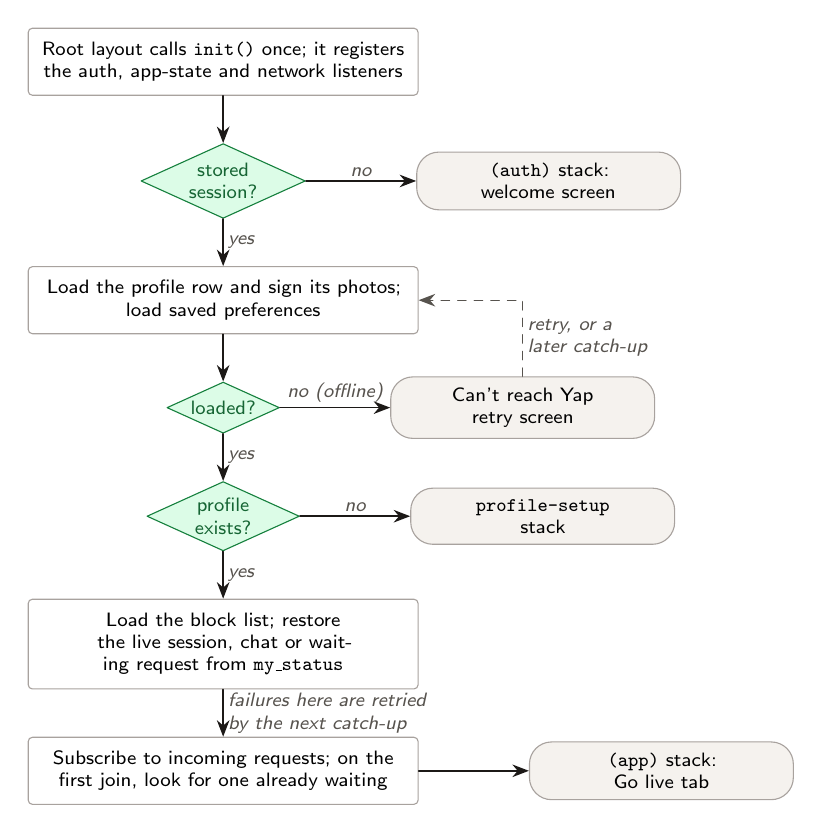
\begin{tikzpicture}[
    node distance=6mm and 9mm,
    st/.style={step=46mm, font=\sffamily\scriptsize},
    outcome/.style={terminal, font=\sffamily\scriptsize, text width=30mm, align=center},
    yes/.style={edgelabel, fill=none, font=\sffamily\scriptsize\itshape, text=muted},
  ]
  \node[st] (init) {Root layout calls \texttt{init()} once; it registers the auth, app-state and network listeners};
  \node[decision, below=of init] (session) {stored\\session?};
  \node[st, below=of session] (profile) {Load the profile row and sign its photos;\\load saved preferences};
  \node[decision, below=of profile] (loaded) {loaded?};
  \node[decision, below=of loaded] (exists) {profile\\exists?};
  \node[st, below=of exists] (extras) {Load the block list; restore the live session, chat or waiting request from \texttt{my\_status}};
  \node[st, below=of extras] (listen) {Subscribe to incoming requests; on the first join, look for one already waiting};

  \node[outcome, right=14mm of session] (welcome) {\texttt{(auth)} stack:\\welcome screen};
  \node[outcome, right=14mm of loaded] (cant) {\ui{Can't reach Yap}\\retry screen};
  \node[outcome, right=14mm of exists] (setup) {\texttt{profile-setup}\\stack};
  \node[outcome, right=14mm of listen] (app) {\texttt{(app)} stack:\\Go live tab};

  \draw[flow] (init) -- (session);
  \draw[flow] (session) -- node[yes, right] {yes} (profile);
  \draw[flow] (session) -- node[yes, above] {no} (welcome);
  \draw[flow] (profile) -- (loaded);
  \draw[flow] (loaded) -- node[yes, right] {yes} (exists);
  \draw[flow] (loaded) -- node[yes, above] {no (offline)} (cant);
  \draw[flow] (exists) -- node[yes, above] {no} (setup);
  \draw[flow] (exists) -- node[yes, right] {yes} (extras);
  \draw[flow] (extras) -- node[yes, right, align=left] {failures here are retried\\by the next catch-up} (listen);
  \draw[flow] (listen) -- (app);
  \draw[softflow] (cant.north) |- node[yes, pos=0.25, right, align=left] {retry, or a\\later catch-up} (profile.east);
\end{tikzpicture}

  \caption{Start-up. The store restores the session and the profile before any screen is shown, then the
    root guards choose the first stack.}
  \label{fig:boot}
\end{figure}

\code{init()} then restores the session that Supabase keeps in AsyncStorage. Without a session, the
guards show the welcome screen. With one, the store loads the user's profile row, signs its photo URLs
and loads the preferences saved on the phone. The profile is loaded before the session is published to
the screens, because a session without a profile means ``new account'' to the root layout, which would
otherwise flash profile setup. If the profile cannot be loaded, typically because the phone is offline at
launch, the store sets \code{loadFailed} and the root layout shows a retry screen instead.

For a user with a profile, the store loads the block list and calls \code{my_status} to restore the
state the app was in when it last closed: a live session (unless a request to go offline is still
waiting to reach the server), an open chat, or a request still waiting for its answer, which it starts
watching again. A failure in this step is tolerated and retried by the next catch-up. Finally the store
subscribes to incoming requests; when that channel first joins, it also looks for a request that arrived
before it was listening.

\section{Account creation, sign-in and password reset}
\label{sec:flow-account}

Yap uses Supabase Auth with email and password. Because the app does not open links, every email the
project sends carries an 8-digit code that the user types into the app (\cref{fig:seq-account}).

\begin{figure}[ht]
  \centering
  % Sequence: creating an account, confirming it and signing in (Figure: account sequence).
\begin{tikzpicture}
  \participant{ui}{0}{Auth screens}
  \participant[actor]{store}{3.5}{Store and\\API layer}
  \participant[serveractor]{auth}{7.0}{Supabase Auth}
  \participant[serveractor]{mail}{10.3}{SMTP sender\\(Resend)}
  \participant[serveractor]{db}{13.5}{Postgres}

  \fragment{ui}{db}{0.35}{7.35}{create an account}
  \msg{ui}{store}{1.0}{\code{signUp}(email, password)}
  \msg{store}{auth}{1.6}{\code{auth.signUp}}
  \msg{auth}{mail}{2.2}{confirmation email}
  \node[font=\sffamily\scriptsize, anchor=west, text=muted] at ($(mail |- 0,-2.2)+(0.15,0.12)$) {8-digit code};
  \msg[reply]{auth}{store}{2.8}{user, no session}
  \msg[reply]{store}{ui}{3.4}{open the code screen}
  \msg{ui}{store}{4.1}{\code{confirmSignUp}(email, code)}
  \msg{store}{auth}{4.7}{\code{verifyOtp}, type signup}
  \msg[reply]{auth}{store}{5.3}{session}
  \msg{store}{db}{5.9}{select own \code{profiles} row}
  \msg[reply]{db}{store}{6.5}{no row}
  \msg[reply]{store}{ui}{7.0}{guard opens profile setup}

  \fragment{ui}{db}{7.75}{12.55}{sign in}
  \msg{ui}{store}{8.4}{\code{signInWithPassword}}
  \msg{store}{auth}{9.0}{\code{auth.signInWithPassword}}
  \msg[reply]{auth}{store}{9.6}{session, or \code{email_not_confirmed}}
  \msg{store}{db}{10.2}{profile, block list, \code{my_status}}
  \msg[reply]{db}{store}{10.8}{rows}
  \msg[reply]{store}{ui}{11.4}{guard opens the app}
  \seqnote{ui}{store}{11.75}{unconfirmed: send a new code, open the code screen}

  \lifelines{12.9}{ui, store, auth, mail, db}
\end{tikzpicture}

  \caption{Creating an account, confirming it with the emailed code, and signing in.}
  \label{fig:seq-account}
\end{figure}

\paragraph{Creating an account} The sign-up screen checks that the password has at least eight
characters and matches its confirmation, then calls \code{signUp}. Supabase creates the user and emails a
confirmation code. If the email already belongs to a confirmed account, Supabase returns a user with no
identities and sends nothing. The app opens the code screen exactly as for a new email, and
\ui{Resend code} behaves the same too, so sign-up never shows whether someone has an account; a note
under the code says \ui{No code? If you already have an account, sign in or reset your password}, with
both as links. If \ui{Confirm email} were
switched off in the dashboard, sign-up would return a session at once and the code screen would be
skipped.

\paragraph{Confirming the email} The code screen accepts exactly eight digits through one hidden input
behind eight boxes, which keeps the operating system's one-time-code autofill working. Because the input
is hidden, \ui{Paste code} (or a long press on the boxes) reads the clipboard, keeps the eight-digit code
from whatever was copied, and fills it in; if there is no code, it says so. The emails show the code on
its own large line so it is easy to copy. The screen submits as soon as the eighth digit arrives. Verifying the code with type \code{signup} returns a
session; the store then loads the (missing) profile and the guards open profile setup. \ui{Resend code}
is disabled for 60 seconds after each send, matching the hosted project's limit of one code per address
per minute (\cref{tab:dashboard}). The local stack allows one per second, so the button's wait is the
only limit there.

\paragraph{Signing in} Sign-in calls \code{signInWithPassword}. If the password is correct but the
account was never confirmed, Supabase answers \code{email_not_confirmed}; the screen then requests a new
code and opens the code screen. Errors are reported as sentences: a wrong password, for example, suggests
\ui{Forgot password}, because accounts created before passwords existed have none.

\paragraph{Resetting a password} \Cref{fig:seq-reset} shows the reset flow. \ui{Forgot password} emails
an 8-digit reset code. The code screen, opened with purpose \code{reset}, only collects the code: it is
checked when the new password is saved, because verifying a recovery code signs the user in. On
\ui{Save and sign in}, the store verifies the code with type \code{recovery}, which creates a session, and
saves the new password with \code{updateUser}. If saving fails, the store signs out locally, so the
recovery session cannot sign the user in on the next launch without a password, and says that the code
has been used up. A signed-in user can also change the password from Settings, which calls
\code{updateUser} directly.

\begin{figure}[ht]
  \centering
  % Sequence: resetting a forgotten password with an emailed code (Figure: reset sequence).
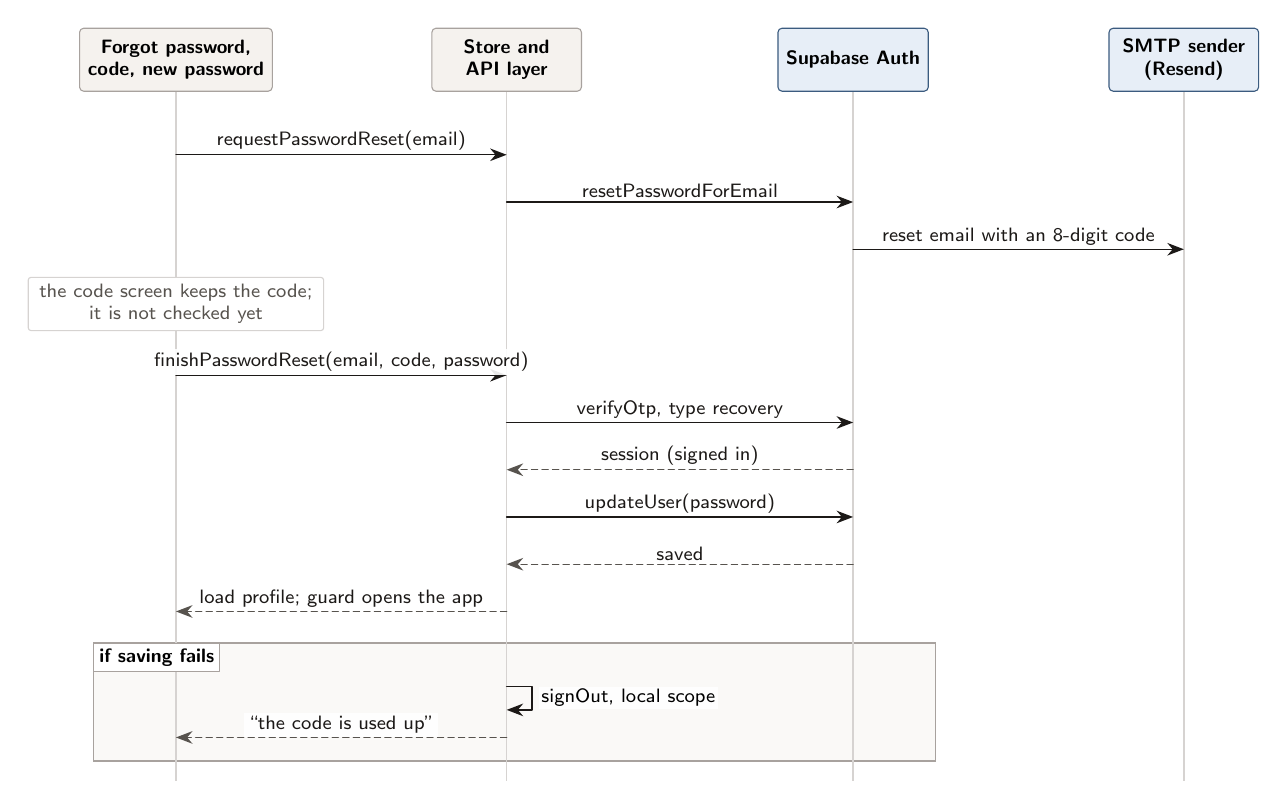
\begin{tikzpicture}
  \participant{ui}{0}{Forgot password,\\code, new password}
  \participant[actor]{store}{4.2}{Store and\\API layer}
  \participant[serveractor]{auth}{8.6}{Supabase Auth}
  \participant[serveractor]{mail}{12.8}{SMTP sender\\(Resend)}

  \msg{ui}{store}{0.8}{\code{requestPasswordReset}(email)}
  \msg{store}{auth}{1.4}{\code{resetPasswordForEmail}}
  \msg{auth}{mail}{2.0}{reset email with an 8-digit code}
  \seqnote{ui}{ui}{2.35}{the code screen keeps the code;\\it is not checked yet}
  \msg{ui}{store}{3.6}{\code{finishPasswordReset}(email, code, password)}
  \msg{store}{auth}{4.2}{\code{verifyOtp}, type recovery}
  \msg[reply]{auth}{store}{4.8}{session (signed in)}
  \msg{store}{auth}{5.4}{\code{updateUser}(password)}
  \msg[reply]{auth}{store}{6.0}{saved}
  \msg[reply]{store}{ui}{6.6}{load profile; guard opens the app}
  \fragment{ui}{auth}{7.0}{8.5}{if saving fails}
  \selfmsg{store}{7.55}{\code{signOut}, local scope}
  \msg[reply]{store}{ui}{8.2}{``the code is used up''}

  \lifelines{8.75}{ui, store, auth, mail}
\end{tikzpicture}

  \caption{Resetting a forgotten password. The emailed code is checked only together with the new
    password.}
  \label{fig:seq-reset}
\end{figure}

\section{Profile setup and saving}
\label{sec:flow-profile}

A signed-in user without a profile row goes through seven screens: a greeting with the 18+ confirmation,
then six numbered steps for the name, gender, introduction, interests, profile picture and further
photos. The answers are kept in the profile draft until the last step, \ui{Finish}, calls the store's
\code{saveProfile}. Editing the profile later uses the same action from a single-page form.
\Cref{fig:seq-profile} shows what saving does.

\begin{figure}[ht]
  \centering
  % Sequence: saving a profile and uploading its photos (Figure: profile sequence).
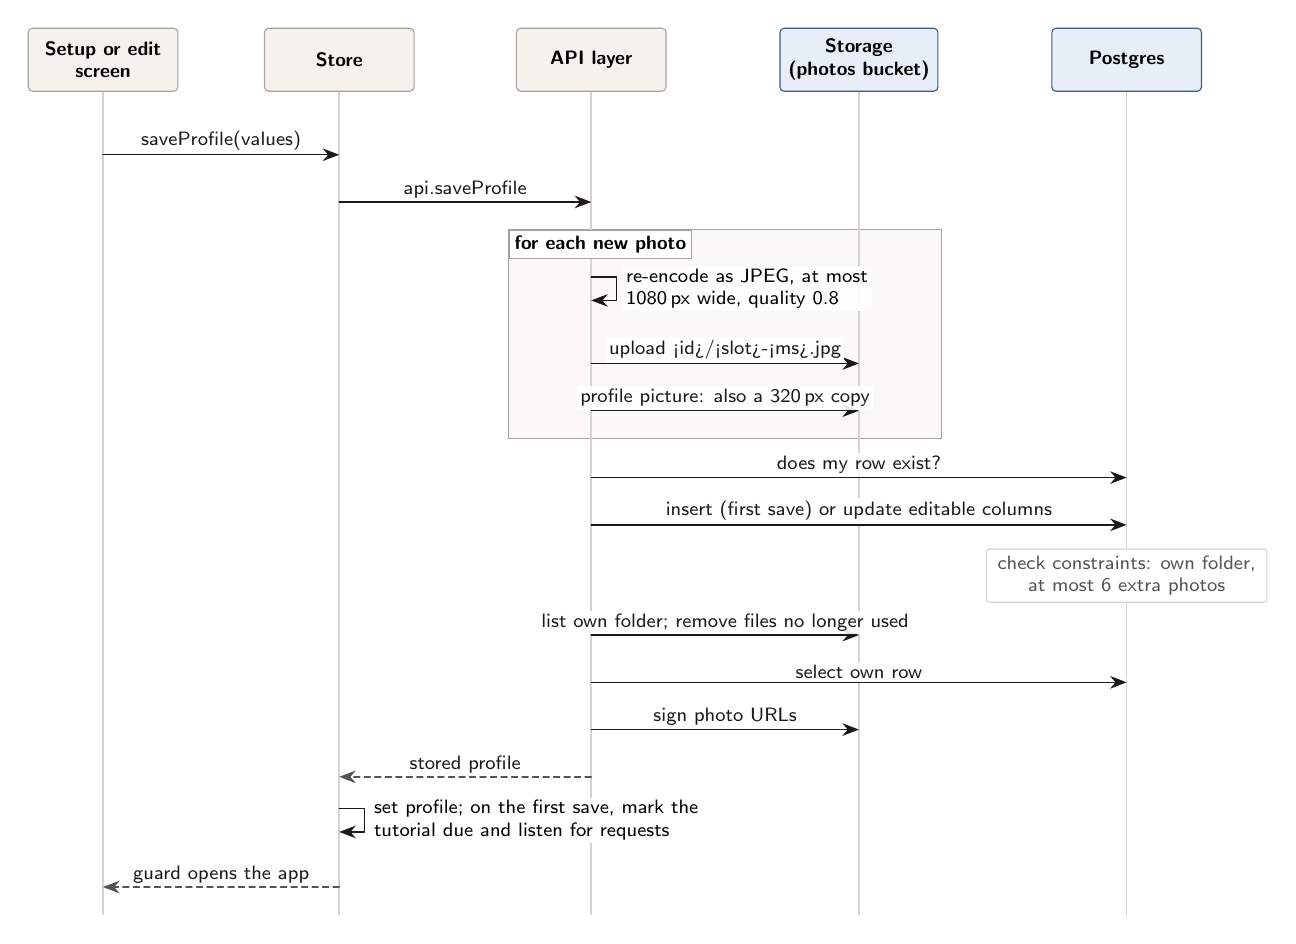
\begin{tikzpicture}
  \participant{ui}{0}{Setup or edit\\screen}
  \participant[actor]{store}{3.0}{Store}
  \participant[actor]{api}{6.2}{API layer}
  \participant[serveractor]{storage}{9.6}{Storage\\(photos bucket)}
  \participant[serveractor]{db}{13.0}{Postgres}

  \msg{ui}{store}{0.8}{\code{saveProfile}(values)}
  \msg{store}{api}{1.4}{\code{api.saveProfile}}
  \fragment{api}{storage}{1.75}{4.4}{for each new photo}
  \selfmsg{api}{2.35}{re-encode as JPEG, at most\\1080\,px wide, quality 0.8}
  \msg{api}{storage}{3.45}{upload \code{<id>/<slot>-<ms>.jpg}}
  \msg{api}{storage}{4.05}{profile picture: also a 320\,px copy}
  \msg{api}{db}{4.90}{does my row exist?}
  \msg{api}{db}{5.50}{insert (first save) or update editable columns}
  \seqnote{db}{db}{5.80}{check constraints: own folder,\\at most 6 extra photos}
  \msg{api}{storage}{6.90}{list own folder; remove files no longer used}
  \msg{api}{db}{7.50}{select own row}
  \msg{api}{storage}{8.10}{sign photo URLs}
  \msg[reply]{api}{store}{8.70}{stored profile}
  \selfmsg{store}{9.10}{set \code{profile}; on the first save, mark the\\tutorial due and listen for requests}
  \msg[reply]{store}{ui}{10.10}{guard opens the app}

  \lifelines{10.45}{ui, store, api, storage, db}
\end{tikzpicture}

  \caption{Saving a profile. Photos are uploaded before the row is written, so the row only ever points
    at files that exist.}
  \label{fig:seq-profile}
\end{figure}

For each photo, the API layer decides whether it is new. A \code{file://} address comes from the picker
or the camera: it is re-encoded as a JPEG at most 1080 pixels wide (never enlarged) at quality 0.8 and
uploaded to \code{<user-id>/<slot>-<milliseconds>.jpg}. The profile picture is also uploaded as a
320-pixel copy for avatars; if that upload fails, avatars fall back to the full photo. An
\code{https://} address is a signed URL of a photo already stored, so its storage path is recovered from
the URL and kept.

The API layer then inserts the row on the first save, or updates only the editable columns afterwards.
It lists the user's folder and removes any file the saved profile no longer uses, such as replaced photos
or uploads from a failed attempt; this tidy-up is best-effort and is retried by the next successful save.
Finally it reloads the row and signs its photo URLs. On the first save, the store marks the tutorial as
due, starts listening for incoming requests, and the guards open the app.

\section{Going live and the nearby list}
\label{sec:flow-live}

\Cref{fig:seq-live} shows the life of a live session from the client's point of view.

\begin{figure}[ht]
  \centering
  % Sequence: going live, refreshing the nearby list and going offline (Figure: live sequence).
\begin{tikzpicture}
  \participant{ui}{0}{Screens and\\app layout}
  \participant[actor]{loc}{3.0}{Phone location}
  \participant[actor]{store}{6.2}{Store and\\API layer}
  \participant[serveractor]{db}{9.8}{Postgres}
  \participant[serveractor]{storage}{13.3}{Storage}

  \msg{ui}{loc}{0.8}{ask for foreground permission}
  \msg[reply]{loc}{ui}{1.4}{position and accuracy}
  \seqnote{loc}{loc}{1.65}{fresh fix within 8\,s, else\\one at most 5 min old}
  \msg{ui}{store}{2.9}{\code{goGreen}(minutes, note, position)}
  \msg{store}{db}{3.5}{\code{go_green}}
  \seqnote{db}{db}{3.8}{relocation rules;\\insert or update the session}
  \msg[reply]{db}{store}{4.9}{server start and end times}
  \msg[reply]{store}{ui}{5.5}{live: button turns red, screen kept awake, end timer set}

  \fragment{ui}{storage}{5.95}{9.4}{loop: every 20 s while live and in the foreground}
  \msg{ui}{store}{6.8}{\code{refreshNearby}}
  \msg{store}{db}{7.4}{\code{nearby}}
  \msg[reply]{db}{store}{8.0}{up to 50 person cards}
  \msg{store}{storage}{8.6}{sign profile pictures (cached)}
  \msg[reply]{store}{ui}{9.15}{nearby list; prompt for new people}

  \fragment{ui}{storage}{9.8}{12.8}{go offline (tap the red button), or the end time is reached}
  \msg{ui}{store}{10.65}{\code{goOffline}}
  \selfmsg{store}{10.9}{clear the live state at once}
  \msg{store}{db}{11.85}{\code{go_offline}: withdraw waiting request, delete session}
  \seqnote{store}{db}{12.15}{on failure: marked pending, retried by the next catch-up}

  \lifelines{13.05}{ui, loc, store, db, storage}
\end{tikzpicture}

  \caption{Going live, keeping the nearby list fresh, and going offline.}
  \label{fig:seq-live}
\end{figure}

\paragraph{Going live} Tapping the green \ui{YAP} button opens the go-live sheet, where the user chooses
30, 60 or 120 minutes and may write a note. On \ui{Go live}, the app asks for foreground location
permission. It never asks for background location. It requests a position with balanced accuracy and
waits up to eight seconds; if no fix arrives, it uses a position the phone recorded in the last five
minutes. The store sends the position, its accuracy, the duration and the note to \code{go_green}, which
applies the relocation rules and writes the session (\cref{sec:relocation-limits}). The function returns
the session's start and end times as the server set them, so the countdown on the button ends when the
session really does, whatever the phone's clock says.

While the user is live, the \code{(app)} layout keeps the screen awake, sets a timer that takes the user
offline at the end time, and polls the nearby list. The button turns red, reads \ui{LIVE} with the
minutes left, and a tap takes the user offline.

\paragraph{The nearby list} One shared list in the store serves the \ui{Nearby} tab, the person sheet and
the nearby prompts. A single poll refreshes it every 20 seconds while the user is live and the app is in
the foreground, and pulling the list down refreshes it at once. Each refresh calls \code{nearby}, which
returns person cards and nothing about where anyone is. The API layer signs the profile pictures and their
small copies in one batch; a person's further photos are signed only when their profile is opened. A
counter discards an answer that arrives after a newer refresh has started.

\paragraph{Nearby prompts} The hook \code{useNearbyAlerts} compares each new list with the people already
announced in this live session. On the first list, if more than one person is there, it shows a summary
(``3 people near you are up for a chat''); after that it announces a newly arrived person by name, the
most recent one if several arrive in the same refresh. Each prompt plays a haptic and disappears after
eight seconds, and each person is announced at most once per session.

\paragraph{Going offline} A tap on the red button, or the end-time timer, calls \code{goOffline}. The store
clears the live state at once and then calls \code{go_offline}, which withdraws the user's waiting request
and deletes the session row. If the call fails when the user chose to go offline, the store records that
the request is pending, shows \ui{Almost offline}, and retries at the next catch-up. If a retry is in
progress when the user goes live again, \code{goGreen} waits for it to finish, so the retry cannot delete
the new session. A session that simply runs out is
also removed by the server's minute job, so a failed call at the end time needs no retry.

\section{Saying hi, answering and chatting}
\label{sec:flow-sayhi}

\subsection{Sending a request and receiving the answer}

A user opens a person from the nearby list or a prompt and taps \ui{Say hi}. The store refuses locally
while the user is in a chat or already has a request waiting; the server applies the same rules and more
(\cref{tab:functions}). \Cref{fig:seq-request} shows the exchange that follows.

\begin{figure}[ht]
  \centering
  % Sequence: a say-hi request and its answer (Figure: request sequence).
\begin{tikzpicture}
  \participant{a}{0}{Sender's app}
  \participant[serveractor]{db}{3.9}{Postgres}
  \participant[serveractor]{rt}{7.8}{Realtime}
  \participant{b}{11.6}{Recipient's app}

  \msg{a}{db}{0.8}{\code{send_request}(target)}
  \seqnote{db}{db}{1.05}{checks; insert \code{pending},\\ends in 5 min}
  \msg[reply]{db}{a}{2.1}{request ID and end time}
  \selfmsg{a}{2.35}{wait: listen for updates,\\poll every 7\,s, give up 3\,s after the end}
  \msg[push]{db}{rt}{3.4}{row inserted}
  \msg[push]{rt}{b}{4.0}{insert where \code{to_user} = recipient}
  \msg{b}{db}{4.6}{\code{request_person}}
  \msg[reply]{db}{b}{5.2}{sender's person card}
  \selfmsg{b}{5.45}{full-screen request,\\5-minute countdown}

  \fragment{a}{b}{6.4}{14.0}{alt}
  \fragguardat{a}{6.75}{[recipient accepts]}
  \msg{b}{db}{7.35}{\code{respond}(accept)}
  \seqnote{db}{db}{7.6}{\code{accepted}; both users \code{chatting}}
  \msg[push]{db}{rt}{8.4}{row updated}
  \msg[push]{rt}{a}{9.0}{status \code{accepted}}
  \seqnote{a}{a}{9.25}{both apps open the chat}
  \fragsep{a}{b}{10.0}{[recipient declines, or nobody answers in time]}
  \msg{b}{db}{10.65}{\code{respond}(decline), or \code{expire_stale}}
  \msg[push]{db}{rt}{11.25}{row updated}
  \msg[push]{rt}{a}{11.85}{status \code{declined} or \code{expired}}
  \seqnote{a}{a}{12.1}{``Not this time''}
  \fragsep{a}{b}{12.85}{[sender cancels]}
  \msg{a}{db}{13.7}{\code{cancel_request}: cancels it, even if just accepted}

  \lifelines{14.25}{a, db, rt, b}
\end{tikzpicture}

  \caption{A say-hi request. The sender learns the outcome from Realtime, from a slow poll, or from its
    own timer, whichever comes first. The server refuses an acceptance after the end time; the timer's
    three seconds of grace only wait for news of an earlier acceptance that is still on its way.}
  \label{fig:seq-request}
\end{figure}

\code{send_request} returns the request's ID and end time, and the sender's app opens the waiting
screen with a five-minute countdown. The store then waits for the answer in three ways at once, so that
one of them always works: a Realtime channel for updates to that request row, a query of its status every
seven seconds, and a timer that gives up three seconds after the end time. The first of these to report
an outcome settles the wait: \code{accepted} opens the chat; any other final status, or the timer, shows
\ui{Not this time}, which reads the same whether the recipient declined or never answered. Separately,
the waiting screen's own countdown shows \ui{Not this time} as soon as the end time arrives. The recipient
cannot accept after the end time: \code{respond} then refuses with \code{request expired}. The three
seconds of grace only wait for news of an acceptance made just before the end time, whose Realtime update
or poll result is still on its way; if it arrives in that window, the chat replaces \ui{Not this time}.
If the sender has already tapped \ui{Back to nearby list}, the store has dropped the request, so the
wait ignores the answer and the next catch-up opens the chat instead.

On the recipient's phone, the insert reaches the app through the incoming-requests channel, which
filters on \code{to_user}. The store fetches the sender's card with \code{request_person} and the
\code{(app)} layout opens a full-screen request with the sender's profile, a countdown, and two buttons of
equal size: \ui{Not now} and \ui{Accept}. While a request is already on screen or the user is in a chat,
later requests are not shown; they expire on the server, and their senders see \ui{Not this time}. If the
recipient's app was in the background or offline when the request arrived, the catch-up finds it by
querying for the newest waiting request addressed to the user.

\paragraph{Accepting} \code{respond} with \code{accept = true} sets the request to \code{accepted} and both
users to \code{chatting}, which removes them from everyone else's nearby list. If the recipient had a
request of their own waiting, the server withdraws it and the app stops showing it. The recipient's app
opens the chat; the sender's app opens it when the update arrives. If the accept fails, for example
because the sender cancelled a moment earlier or is no longer live, the recipient sees a short
explanation.

\paragraph{Cancelling} \ui{Cancel request} on the waiting screen removes the request from the screen at
once and calls \code{cancel_request}. If that call fails, the request reappears, the app resumes watching
for the answer, and an alert explains that the user is still waiting. If the cancel reaches the server
just after an accept, the server ends that chat too, so nobody is left in a chat the other person never
sees.

\subsection{The one-to-one chat}

Both apps open the chat in the same way (\cref{fig:seq-chat}): the store subscribes to the chat's
channel first and loads the newest 200 messages each time the channel joins, so a message sent between
the two steps is not lost. The chat screen shows the partner's photo and name, a safety tip during the user's first few chats, and
a message composer. Tapping the partner's name opens their profile, including the live note that often
says where to find them.

\begin{figure}[ht]
  \centering
  % Sequence: the one-to-one chat, from opening to ending (Figure: chat sequence).
\begin{tikzpicture}
  \participant{a}{0}{User A's app}
  \participant[serveractor]{db}{4.3}{Postgres}
  \participant[serveractor]{rt}{8.6}{Realtime}
  \participant{b}{12.9}{User B's app}

  \msg{a}{rt}{0.8}{join \code{chat-<id>}: messages, request updates}
  \msg[reply]{rt}{a}{1.4}{subscribed}
  \msg{a}{db}{2.0}{newest 200 messages; request status}
  \msg[reply]{db}{a}{2.6}{history}
  \seqnote{a}{b}{2.95}{B's app opens the chat in the same way}
  \msg{a}{db}{4.0}{\code{send_chat_message}(id, text)}
  \msg[reply]{db}{a}{4.6}{saved row, shown at once}
  \msg[push]{db}{rt}{5.2}{row inserted}
  \msg[push]{rt}{b}{5.8}{new message}
  \msg[push]{rt}{a}{6.4}{same message, skipped by ID}
  \msg{b}{db}{7.2}{\code{end_chat}(id, met or cancelled)}
  \seqnote{db}{db}{7.45}{status set; both users\\\code{open} again}
  \msg[push]{db}{rt}{8.5}{row updated}
  \msg[push]{rt}{a}{9.1}{status no longer \code{accepted}}
  \selfmsg{a}{9.35}{``B ended the chat'';\\composer closed}
  \seqnote{a}{b}{10.35}{a block ends the chat in the same way; if B deletes the account, A's app notices at its next catch-up or send}

  \lifelines{10.85}{a, db, rt, b}
\end{tikzpicture}

  \caption{The one-to-one chat. Messages are merged by ID, so the copy that Realtime delivers to the
    sender is ignored.}
  \label{fig:seq-chat}
\end{figure}

\code{send_chat_message} returns the saved row, which the sender's app shows immediately; when Realtime
delivers the same row a moment later it is recognised by its ID and skipped. Messages are kept sorted by
the time the server stored them.

\paragraph{Ending the chat} \ui{End} asks \ui{Did you meet?} with three choices: \ui{Keep chatting},
\ui{We met} and \ui{End chat}. The two ending choices close the chat on this phone at once and call
\code{end_chat} with outcome \code{met} or \code{cancelled}; both users return to the nearby lists if they
are still live. The other phone learns of the end through the chat channel, which also listens for
updates to the request row: when the status leaves \code{accepted}, the chat stays on screen with the
notice that the partner ended it and the composer replaced by that notice. Leaving the chat screen without
ending it keeps the chat open; a bar on the \ui{Go live} and \ui{Nearby} tabs reopens it.

\paragraph{Chats nobody ends} If both users simply stop using the app, the minute job ends the chat once
neither of them is live (\cref{sec:housekeeping}), and \code{my_status} no longer offers it after a
restart.

\section{Events and group chats}
\label{sec:flow-events}

\Cref{fig:seq-events} traces the event features.

\begin{figure}[ht]
  \centering
  % Sequence: loading, creating and joining events, and the group chat (Figure: events sequence).
\begin{tikzpicture}
  \participant{ui}{0}{Map and\\event screens}
  \participant[actor]{loc}{3.2}{Phone location}
  \participant[actor]{store}{6.5}{Store and\\API layer}
  \participant[serveractor]{db}{10.1}{Postgres}
  \participant[serveractor]{rt}{13.6}{Realtime}

  \msg{ui}{loc}{0.8}{permission (asked once) and position}
  \msg[reply]{loc}{ui}{1.4}{recent, fresh or last known position}
  \msg{ui}{store}{2.0}{\code{loadEvents}(centre)}
  \msg{store}{db}{2.6}{\code{events_near}(lat, lng, radius 1--50\,km)}
  \msg[reply]{db}{store}{3.2}{up to 50 event cards}
  \msg[reply]{store}{ui}{3.8}{pins and the radius circle}

  \fragment{ui}{rt}{4.2}{6.8}{create: long-press the map, or ``Create event here''}
  \msg{ui}{store}{5.05}{\code{createEvent}(category, title, details, place, start)}
  \msg{store}{db}{5.65}{\code{create_event}: host becomes a member}
  \msg[reply]{db}{store}{6.25}{event card; the group chat opens}

  \fragment{ui}{rt}{7.2}{10.4}{join: tap a pin, then ``Join and open chat''}
  \msg{ui}{loc}{8.05}{position}
  \msg{ui}{store}{8.65}{\code{joinEvent}(id, position)}
  \msg{store}{db}{9.25}{\code{join_event}: within 5\,km}
  \msg[reply]{db}{store}{9.85}{member; the group chat opens}

  \fragment{ui}{rt}{10.8}{13.9}{group chat, while its screen is open}
  \msg{store}{rt}{11.65}{join \code{messages-event_id-<id>}}
  \msg{store}{db}{12.25}{newest 200 messages; \code{send_event_message}}
  \msg[push]{rt}{store}{12.85}{new messages from members}
  \msg[reply]{store}{ui}{13.45}{thread, minus blocked senders}

  \lifelines{14.15}{ui, loc, store, db, rt}
\end{tikzpicture}

  \caption{Loading events around the user, creating, joining and deleting an event, and the group chat.}
  \label{fig:seq-events}
\end{figure}

\paragraph{Finding events} When the \ui{Map} tab opens, and each time its tab button is pressed, the
screen finds the user. It asks for location permission only if the user has never decided, uses a
position the phone recorded in the last two minutes if there is one, otherwise waits up to eight seconds
for a fresh fix. If neither comes, it only centres the map on the last position the phone knows, however
old, and shows that it could not find the user: an old position is never sent to the server, which would
otherwise hold it as the user's last known position and refuse the real one. With a recent or fresh
position it centres the map and loads the events within the chosen radius of that point: the store sends
the position to \code{set_map_position} and then calls \code{events_near}, which lists events around the
position the server holds (\cref{sec:location-privacy}). If the server refuses the new position because it is too
far from the last known one or changed too often, the map keeps the pins it has and shows the refusal
under the banner with a \ui{Try again} button. Without a position, the
map loads no events and shows a note and a button to turn location on; when the user returns from the
phone's settings, the map tries again.

The radius is chosen with a slider from 1 to 50 kilometres (default 10) and drawn on the map as a circle.
Releasing the slider saves the value for the account, fits the map to the circle, and lists the events
again with \code{events_near} alone, around the position the server already holds: no position is sent
again, so one the phone found a while ago can never replace a newer one. \code{events_near} applies the radius on the server and never searches beyond 50
kilometres. Each event becomes a pin showing its category icon and title; events the user has joined are
drawn in green. If none are in range, a note suggests widening the distance or creating an event.

\paragraph{Creating an event} A long press on the map, or \ui{Create event here} for the centre of the
current view, opens the event form at that place. The host picks one of twelve categories, writes a title
and optional details, and picks a start time from now to seven days ahead; on Android the picker asks for
the date and then the time. \code{create_event} stores the event, adds the host as a member and returns
the event card, and the app opens the event's group chat.

\paragraph{Joining} Tapping a pin opens the event sheet with the category, title, start time
(\ui{Starts in 25 min}, \ui{Started 10 min ago}), number of members, details and host. \ui{Join and open
chat} requests the phone's position, sends it to \code{set_map_position}, and calls \code{join_event},
which accepts the user only within five kilometres of the position the server holds. A user therefore
sees events up to 50 kilometres from their own position, but only someone nearby can join one and read
its chat. The host's photo is sent only to people who joined, so after a join the app lists the pins
again with \code{events_near} alone to show it. If the host has deleted the event in the meantime, the server
answers \code{no such event}; the app takes the event off the map and the sheet shows \ui{This event was
deleted}.

\paragraph{The group chat} The group chat subscribes to the event's messages while its screen is open and
loads the newest 200 messages each time the channel joins. Messages show the sender's name. Messages from
users the reader has blocked are excluded by row-level security and filtered again on screen. A long press
on someone else's message offers \ui{Report} and \ui{Block}; blocking the host also removes the event from
the map and closes the chat. A guest can leave the event, which removes their membership and their access
to its chat. The host has no \ui{Leave} button, because on the server a host leaving deletes the event;
the host deletes it deliberately instead. Sending to the chat of an event that no longer exists, or that
the user has left, is refused with \code{not a member}, shown as \ui{You can't post here. The event may
have ended or been deleted.}

\paragraph{Deleting an event} The event sheet shows the host a \ui{Delete event} button. After a
confirmation (\ui{Delete this event?} \ui{Everyone who joined will lose the group chat.}), the store
calls \code{delete_event}, which accepts only the host. Deleting the row removes the event's members and
its group-chat messages through their cascading foreign keys. The app takes the event off the map at once;
other phones stop showing it at their next load of events. An event already deleted, for example from
another phone, counts as deleted.

\section{Photos}
\label{sec:flow-photos}

Uploading photos is part of saving a profile (\cref{sec:flow-profile}). Showing another user's photo
takes a signed URL, because the bucket is private (\cref{fig:seq-photos}).

\begin{figure}[ht]
  \centering
  % Sequence: showing another user's photo through a signed URL (Figure: photo sequence).
\begin{tikzpicture}
  \participant{ui}{0}{List or\\profile screen}
  \participant[actor]{api}{3.3}{API layer\\(URL cache)}
  \participant[serveractor]{storage}{6.9}{Storage}
  \participant[serveractor]{db}{10.4}{Postgres\\read policy}
  \participant[actor]{img}{13.8}{Image cache}

  \msg{ui}{api}{0.8}{photo paths of the cards}
  \selfmsg{api}{1.05}{skip paths with a URL that has 10 min\\left, or a refusal under 1 min old}
  \msg{api}{storage}{2.1}{\code{createSignedUrls}(the rest, 1 h)}
  \msg{storage}{db}{2.7}{select policy \code{photos_read_visible}}
  \selfmsg{db}{2.95}{\code{can_see_photo}\\for each file}
  \msg[reply]{db}{storage}{3.9}{allowed or not}
  \msg[reply]{storage}{api}{4.5}{a URL for each allowed path}
  \selfmsg{api}{4.75}{cache: a URL for 1 h,\\a refusal for 60\,s}
  \msg[reply]{api}{ui}{5.7}{display URLs}
  \msg{ui}{img}{6.3}{show, with the token removed from the cache key}
  \msg{img}{storage}{6.9}{download only on a cache miss}

  \lifelines{7.25}{ui, api, storage, db, img}
\end{tikzpicture}

  \caption{Showing another user's photo. Storage signs a URL only if the read policy allows the signed-in
    user to see the file.}
  \label{fig:seq-photos}
\end{figure}

The API layer keeps a cache from storage path to signed URL. A URL is created for fifteen minutes and
reused until fewer than five minutes remain, so the same photo keeps the same URL across refreshes. A path that
could not be signed, because the file does not exist or its owner is not visible to the user, is
remembered for one minute and then asked for again, so the photo appears soon after its owner becomes
visible. Expired entries are dropped whenever new URLs are signed, and the whole cache is cleared on
sign-out. All the paths a screen needs are signed in one request.

Storage signs a URL only if the user may read the object. The read policy calls
\code{private.can_see_photo}, which allows a photo only while its owner is visible to the user
(\cref{sec:photo-privacy}). On the device, \code{expo-image} caches the downloaded image under the URL
without its token, so re-signing a URL does not cause the image to be downloaded again.

\section{Account deletion}
\label{sec:flow-delete}

\ui{Delete account} in Settings opens a screen that lists what is deleted. Its \ui{Delete my account}
button only works once the user has typed their first name as it is on their profile (ignoring capitals
and spaces around it), so a stray tap cannot delete an account. The app checks for a connection first,
so a dropped network cannot remove the photos and leave the account, and a second tap waits for the
first. It then runs the sequence in \cref{fig:seq-delete}. The photos are removed first, through the Storage API, because once the account is
gone the session can no longer reach Storage, and Supabase does not allow deleting rows from the storage
tables directly.

\begin{figure}[ht]
  \centering
  % Sequence: deleting an account (Figure: deletion sequence).
\begin{tikzpicture}
  \participant{ui}{0}{Settings}
  \participant[actor]{store}{3.5}{Store and\\API layer}
  \participant[serveractor]{storage}{6.9}{Storage}
  \participant[serveractor]{db}{10.2}{Postgres}
  \participant[serveractor]{auth}{13.6}{Supabase Auth}

  \selfmsg{ui}{0.6}{confirm:\\``Delete your account?''}
  \msg{ui}{store}{1.6}{\code{deleteAccount}}
  \msg{store}{storage}{2.2}{list own folder, 100 at a time}
  \msg[reply]{storage}{store}{2.8}{paths}
  \msg{store}{storage}{3.4}{remove every file}
  \msg{store}{db}{4.0}{\code{delete_account}}
  \selfmsg{db}{4.25}{chat partner back to \code{open};\\delete the \code{auth.users} row;\\every user table cascades}
  \msg[reply]{db}{store}{5.6}{done}
  \msg{store}{auth}{6.2}{\code{signOut}}
  \selfmsg{store}{6.45}{auth listener: close channels,\\forget URLs, reset state}
  \msg[reply]{store}{ui}{7.4}{guard opens the welcome screen}

  \lifelines{7.75}{ui, store, storage, db, auth}
\end{tikzpicture}

  \caption{Deleting an account. Removing the Auth user removes every row that belongs to the user, except
    the reports, which are kept without it.}
  \label{fig:seq-delete}
\end{figure}

\code{delete_account} first puts the user's email address on the ban list if the account is hidden or
suspended (\cref{sec:signup-checks}), and returns the user's chat partner, if any, to \code{open}, so
the partner can be found and can say hi again; then it deletes the Auth user. Every user foreign key
except the two in \code{reports} cascades, so the delete removes the profile, the live session and map
position, every request sent or received with its messages, every event hosted with its members and
messages, every membership, every message sent, every block made or received, the location-change log,
the event-post log and the call counts. Reports made or received stay, with the user's id set to null
(\cref{sec:blocking-reporting}). The app then
signs out and forgets what the phone saved for the account, and the Auth listener resets the store to its
initial state, closes every channel and clears the image cache.

\chapter{Features}
\label{ch:features}

This chapter describes every feature of the app: what the user sees, what happens, and where it is
implemented. Each feature ends with a summary of its screens (under \code{src/app}), the client functions
that carry it, and the server rules that enforce it. The data flows behind the larger features are traced
in \cref{ch:flows}; this chapter refers to them rather than repeating them. \Cref{fig:screen-map} shows
how the signed-in screens connect, and \cref{app:routes} lists every route.

\begin{figure}[ht]
  \centering
  % Screen map: how the signed-in screens connect, with the action on each transition (Figure: screen map).
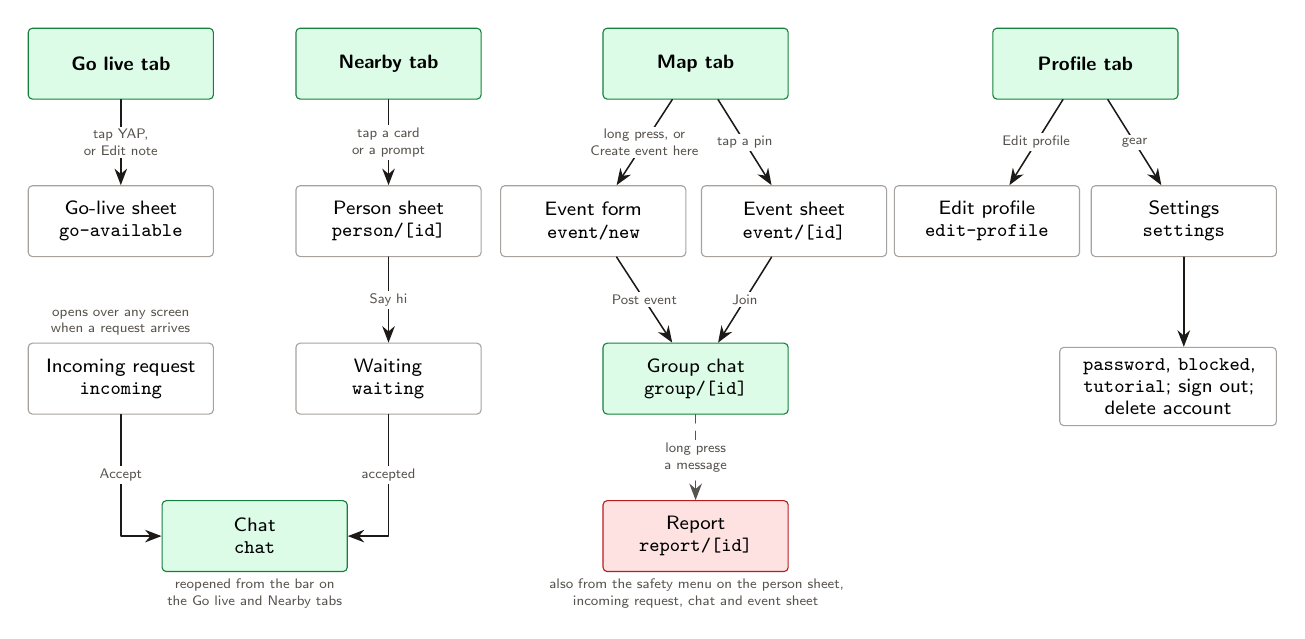
\begin{tikzpicture}[
    tab/.style={box, accentbox, font=\sffamily\scriptsize\bfseries, text width=20mm, minimum height=9mm, align=center},
    scr/.style={box, font=\sffamily\scriptsize, text width=20mm, minimum height=9mm, align=center},
    act/.style={font=\sffamily\tiny, text=muted, fill=white, inner sep=1pt, align=center},
  ]
  \node[tab] (golive) at (1.2,0) {Go live tab};
  \node[tab] (nearby) at (4.6,0) {Nearby tab};
  \node[tab] (map) at (8.5,0) {Map tab};
  \node[tab] (profile) at (13.45,0) {Profile tab};

  \node[scr] (sheet) at (1.2,-2.0) {Go-live sheet\\\texttt{go-available}};
  \node[scr] (person) at (4.6,-2.0) {Person sheet\\\texttt{person/[id]}};
  \node[scr] (waiting) at (4.6,-4.0) {Waiting\\\texttt{waiting}};
  \node[scr] (incoming) at (1.2,-4.0) {Incoming request\\\texttt{incoming}};
  \node[scr, accentbox] (chat) at (2.9,-6.0) {Chat\\\texttt{chat}};
  \node[scr] (newev) at (7.2,-2.0) {Event form\\\texttt{event/new}};
  \node[scr] (event) at (9.75,-2.0) {Event sheet\\\texttt{event/[id]}};
  \node[scr, accentbox] (group) at (8.5,-4.0) {Group chat\\\texttt{group/[id]}};
  \node[scr, draw=alert, fill=alertsoft] (report) at (8.5,-6.0) {Report\\\texttt{report/[id]}};
  \node[scr] (edit) at (12.2,-2.0) {Edit profile\\\texttt{edit-profile}};
  \node[scr] (settings) at (14.7,-2.0) {Settings\\\texttt{settings}};
  \node[scr, text width=24mm, align=center] (rows) at (14.5,-4.1) {\texttt{password}, \texttt{blocked},\\\texttt{tutorial}; sign out;\\delete account};

  \draw[flow] (golive) -- node[act] {tap YAP,\\or Edit note} (sheet);
  \draw[flow] (nearby) -- node[act] {tap a card\\or a prompt} (person);
  \draw[flow] (person) -- node[act] {Say hi} (waiting);
  \draw[flow] (waiting) |- node[act, pos=0.25] {accepted} (chat.east);
  \draw[flow] (incoming) |- node[act, pos=0.25] {Accept} (chat.west);
  \draw[flow] (map) -- node[act] {long press, or\\Create event here} (newev);
  \draw[flow] (map) -- node[act] {tap a pin} (event);
  \draw[flow] (newev) -- node[act] {Post event} (group);
  \draw[flow] (event) -- node[act] {Join} (group);
  \draw[flow] (profile) -- node[act] {Edit profile} (edit);
  \draw[flow] (profile) -- node[act] {gear} (settings);
  \draw[flow] (settings) -- (settings |- rows.north);
  \draw[softflow] (group) -- node[act] {long press\\a message} (report);

  \node[act, anchor=south, text width=22mm, fill=none] at ($(incoming.north)+(0,0.05)$) {opens over any screen\\when a request arrives};
  \node[act, anchor=north, text width=46mm, fill=none] at ($(report.south)+(0,-0.05)$) {also from the safety menu on the person sheet,\\incoming request, chat and event sheet};
  \node[act, anchor=north, text width=40mm, fill=none] at ($(chat.south)+(0,-0.05)$) {reopened from the bar on the Go live and Nearby tabs};
\end{tikzpicture}

  \caption{Screen map of the signed-in app. Green boxes along the top are the four tabs; arrows carry the
    action that opens the next screen. The incoming request and the chat can open over any screen.}
  \label{fig:screen-map}
\end{figure}

\section{Welcome and account creation}
\label{sec:feature-signup}

The welcome screen shows the name \ui{Yap}, the line \ui{The app that gets you off the app}, and two
buttons: \ui{Create account} and \ui{Sign in}. A note states that continuing means agreeing to the
Community Guidelines and Privacy Policy. \ui{Create account} asks for an email address, a password and its
confirmation. Above its button, a line says that creating an account means agreeing to the Terms of
Service and the Community Guidelines and confirming the Privacy Policy has been read; each name is a link
(the terms and privacy policy open in the browser, the guidelines in the app). The button then opens the
code screen (\cref{sec:flow-account}). The code screen shows eight boxes,
fills them as digits are typed or pasted, submits on the eighth digit, and offers \ui{Resend code} after
a 60-second countdown.

\implemented
  {\code{(auth)/welcome}, \code{(auth)/sign-up}, \code{(auth)/verify}}
  {\code{signUp}, \code{confirmSignUp}; \code{api.resendSignUpCode}; \code{passwordProblem}}
  {Supabase Auth: email confirmation on, minimum password length 8, 8-digit code in the confirmation template}

\section{Signing in and passwords}

\ui{Sign in} takes an email and a password. An unconfirmed account is sent a new code and taken to the
code screen. \ui{Forgot password?} carries the typed email to the reset screen, which emails a reset code;
the code screen then leads to \ui{Choose a new password}, and saving signs the user in
(\cref{sec:flow-account}). A note on the sign-in screen tells users who signed up with an emailed code
alone, before passwords existed, to set a password this way. Signed-in users change their password from
\ui{Settings}, \ui{Change password}; a success alert confirms the change. A new password must have
at least eight characters and match its confirmation before anything is sent.

\implemented
  {\code{(auth)/sign-in}, \code{(auth)/forgot-password}, \code{(auth)/verify}, \code{(auth)/new-password}, \code{(app)/password}}
  {\code{signInWithPassword}, \code{finishPasswordReset}; \code{api.requestPasswordReset}, \code{api.setPassword}}
  {Supabase Auth: password sign-in, recovery codes, at most one code per address per minute on the hosted project (\cref{tab:dashboard})}

\section{Profile setup}
\label{sec:feature-setup}

A new account first sees a greeting and must tick \ui{I'm 18 or older} before continuing. Six numbered
steps follow, one question per screen, each with a progress bar and its number:

\begin{enumerate}
  \item first and last name; the screen notes that others see only the first name and last initial;
  \item gender (woman, man, non-binary or prefer not to say) and a switch to show it on the profile, which
    is disabled for \ui{Prefer not to say};
  \item an introduction of up to 300 characters;
  \item three to five interests from a list of 32;
  \item a profile picture, chosen from the library or taken with the front camera, cropped square;
  \item four to six further photos, picked several at a time, each of which can be replaced or removed.
\end{enumerate}

\ui{Finish} saves the profile (\cref{sec:flow-profile}). The greeting also offers
\ui{Use a different account}, which signs out, for someone who signed up with the wrong address.

\implemented
  {\code{profile-setup/index}, \code{name}, \code{gender}, \code{about}, \code{interests}, \code{photo}, \code{photos}}
  {\code{ProfileDraftProvider}, \code{saveProfile}, \code{api.saveProfile}; \code{PhotoGrid}, \code{SetupStep}}
  {\code{profiles} check constraints (lengths; names and intro with something visible and no control characters, direction overrides or stacked accents; 3 to 5 different interests of 1 to 30 characters; own-folder photo paths; at most 6 extra photos); insert policy requires \code{is_adult}}

\section{Profile tab and editing}

The \ui{Profile} tab shows the user's profile exactly as other people see it, built by
\code{asSeenByOthers} from the stored profile: first name and last initial, gender only if shown, the live
note while the user is live, the further photos, the introduction and the interests. A gear opens
\ui{Settings} and \ui{Edit profile} opens a single-page form with every setup field except the 18+
confirmation, which keeps its original answer. The form lists anything still missing (\ui{Add at least 4
more photos, \dots{} to continue}) and saves through the same action as setup.

\implemented
  {\code{(app)/(tabs)/profile}, \code{(app)/edit-profile}}
  {\code{ProfileForm}, \code{PersonDetails}, \code{asSeenByOthers}, \code{saveProfile}}
  {Column grants: a client may update only the editable profile columns}

\section{Going live}
\label{sec:feature-live}

The \ui{Go live} tab holds one large round button. Green, it reads \ui{YAP}; tapping it opens the go-live
sheet. There the user picks 30, 60 or 120 minutes (60 is preselected) and may add a note of up to 60
characters, with a counter. A notice explains that the location is used only to find people in the same
place while the user is available, that nobody sees it, and that it is deleted on stopping. If location
permission is refused, the notice changes to a warning and the button to \ui{Open Settings}.

While the user is live the button is red and reads \ui{LIVE}, the minutes left and \ui{Tap to get off};
its pulsing ring speeds up. Below it the note appears with \ui{Edit} (or \ui{Add} when empty), which opens
the same sheet in edit mode; saving the note updates the screen at once and restores the old note if the
server refuses. A caption reminds the user to keep Yap open to receive requests, and the screen stays on.
When the time runs out, the user goes offline and a dismissible \ui{Your time's up} notice appears.

\implemented
  {\code{(app)/(tabs)/index}, \code{(app)/go-available}}
  {\code{HeroButton}, \code{DurationChips}, \code{useForegroundLocation}, \code{goGreen}, \code{updateNote}, \code{goOffline}; keep-awake and the end timer in \code{(app)/_layout}}
  {\code{go_green} (durations, note length, relocation limits), \code{update_note}, \code{go_offline}; \code{expire_stale} ends sessions on time}

\section{Nearby list and prompts}
\label{sec:feature-nearby}

The \ui{Nearby} tab requires the user to be live, because only people who can see each other appear to
each other; otherwise it shows the Yap cat and a \ui{Go live} button. While live, it shows \ui{You're live,
47 min left} and a card for each nearby person: photo, first name and last initial, a \ui{here now} badge,
the note, two lines of introduction and up to three interests. Placeholder cards pulse while the first
list loads; an empty list shows \ui{Nobody else is green here yet}. Above the list, a bar shows a chat in
progress and another the request the user is waiting on, with its countdown, or \ui{Not this time} once
it has ended. While live, a prompt slides in at the top of any screen when someone new is nearby, with
\ui{Say hi} or \ui{See them} (\cref{sec:flow-live}).

\implemented
  {\code{(app)/(tabs)/nearby}; prompts in \code{(app)/_layout}}
  {\code{useNearbyPolling}, \code{useNearby}, \code{refreshNearby}, \code{useNearbyAlerts}, \code{NearbyToast}, \code{PersonCard}}
  {\code{nearby}: live, open, active users in the same cell of about 100\,m or a touching one, no blocks, at most 50, cards only, 12 calls a minute}

\section{Person sheet and saying hi}

Opening a person shows a sheet with their full profile: large photo, name, gender if shown, note, further
photos (signed only now), introduction and interests, with the safety menu in the corner. The sheet looks
the person up in the shared nearby list, the current chat partner or the sender of the request on screen;
if they have gone, it says \ui{They're not live any more}. The footer offers \ui{Say hi}, unless the user is
already chatting (with this person or anyone else) or has a request waiting, in which case it explains
why. A sent request replaces the sheet with the waiting screen.

\implemented
  {\code{(app)/person/[id]}}
  {\code{PersonDetails}, \code{usePersonPhotos}, \code{sayHi}, \code{api.sendRequest}}
  {\code{send_request}: proximity, blocks, one request waiting, one chat, 5 requests per 10 minutes}

\section{Waiting for an answer}

The waiting screen shows the recipient's photo with the Yap cat beside it, \ui{Waiting for Sam\dots},
\ui{They have 5 minutes to answer} and a countdown, with a reassurance that \ui{Not this time} carries no
score. \ui{Back to nearby list} leaves it open in the background, where the bar on the Nearby tab tracks
it. \ui{Cancel request} withdraws it on the server. When the answer is no, or time runs out, the screen
changes to \ui{Not this time} (\cref{sec:flow-sayhi}).

\implemented
  {\code{(app)/waiting}}
  {\code{watchAnswer}, \code{api.waitForAnswer}, \code{cancelRequest}, \code{expireOutgoing}, \code{clearOutgoing}}
  {\code{cancel_request}; \code{expire_stale} expires the request after five minutes or when the sender stops being live}

\section{Answering a request}

An incoming request takes over the screen wherever the user is, with a haptic. It shows \ui{Someone wants
to chat}, the sender's full profile and the time left to answer, and offers \ui{Not now} and \ui{Accept}
with equal size and weight. The safety menu is in the corner. The screen cannot be swiped away; it closes
when the user answers, when the time runs out, or when the user blocks the sender.

\implemented
  {\code{(app)/incoming}; opened by \code{(app)/_layout}}
  {\code{listenForRequests}, \code{onIncoming}, \code{respondToIncoming}, \code{expireIncoming}}
  {\code{respond}: one chat per user, the sender still live; \code{request_person}: card hidden after a block}

\section{One-to-one chat}

An accepted request opens the chat for both users. The header shows the partner's photo and name with
\ui{Your yap partner --- go say hi}; tapping it opens their profile. A new chat shows the happy Yap cat
above the first message, and in a user's first chats a safety tip, shown until it has been seen three
times, advises meeting in the public place both are in. Messages up to 1000 characters are sent with the arrow button; the user's own messages
are green and on the right. \ui{End} asks whether the two met. If the partner ends the chat, the
composer is replaced by \ui{Sam ended the chat} and \ui{End} becomes \ui{Close}. The chat survives leaving
the screen, and a bar on the \ui{Go live} and \ui{Nearby} tabs reopens it (\cref{sec:flow-sayhi}).

\implemented
  {\code{(app)/chat}}
  {\code{openChat}, \code{api.subscribeChat}, \code{sendMessage}, \code{endChat}, \code{markChatEnded}; \code{ChatThread}, \code{ActiveChatBar}}
  {\code{send_chat_message} (length, membership, blocks, 30 per minute), \code{end_chat}; Realtime delivery limited by the \code{messages} policy}

\section{Map and events}
\label{sec:feature-events}

The \ui{Map} tab shows events around the user. A banner explains that pins show events and never people,
and holds the distance slider (1 to 50\,km). A button above \ui{Create event here} recentres the map on
the user. Pins show the event's category icon and title; joined events are green. The event form, the
event sheet and the group chat behave as described in \cref{sec:flow-events}. \Cref{tab:event-rules}
summarises who may do what.

\begin{table}[ht]
  \centering
  \caption{Event rules.}
  \label{tab:event-rules}
  \tablefont
  \begin{tabularx}{\textwidth}{@{}L{34mm}Y@{}}
    \toprule
    \textsf{\textbf{Action}} & \textsf{\textbf{Rule}} \\
    \midrule
    See an event & Within the chosen radius, at most 50\,km, of the position the server holds for the user; until three hours after its start; host active and not blocked either way; the host's photo only after joining \\
    Create an event & Active adult profile; one of the twelve categories; start from five minutes ago to seven days ahead; at most five per host in 24 hours \\
    Join an event & Active adult profile; within 5\,km of the position the server holds; not blocked by or blocking the host \\
    Read and write its chat & Members only; 1 to 1000 characters; at most 30 messages a minute \\
    Leave & A guest's membership ends; the app offers no \ui{Leave} to the host \\
    Delete & Host only, from the event sheet, after a confirmation; members and the group chat go with the event \\
    \bottomrule
  \end{tabularx}
\end{table}

\implemented
  {\code{(app)/(tabs)/map}, \code{(app)/event/new}, \code{(app)/event/[id]}, \code{(app)/group/[id]}}
  {\code{loadEvents}, \code{setEventRadius}, \code{createEvent}, \code{joinEvent}, \code{leaveEvent}, \code{deleteEvent}, \code{enterEventChat}, \code{sendGroupMessage}; \code{EventIcon}, \code{eventCategory}}
  {\code{set_map_position}, \code{events_near}, \code{create_event}, \code{join_event}, \code{leave_event}, \code{delete_event}, \code{send_event_message}}

\section{Blocking and reporting}
\label{sec:feature-safety}

Every surface that shows another person (the person sheet, the incoming request, the chat and the event
sheet) has a menu with \ui{Report} and \ui{Block}; in a group chat, a long press on a message offers the
same. Blocking asks for confirmation, then takes effect on the server first: the block is recorded and any
request or chat between the two is ended. The app then drops the person from the nearby list, the map and
any request or chat on screen. \ui{Report} offers six reasons, an optional comment of up to 500 characters
and \ui{Also block}, which is ticked by default. The form says that every report is reviewed and that the
reported person will not know who reported them. \ui{Settings}, \ui{Blocked people} lists blocked
users by first name and last initial, with \ui{Unblock}. The server semantics are in
\cref{sec:blocking-reporting}. Separately, the server refuses an introduction, interest, live note, event
or message that contains a slur or abusive word from its list, and the app explains why
(\cref{sec:word-filter}); the owner reviews reports and can suspend an account (\cref{sec:moderation}).
A hidden or suspended user sees \ui{Your account is on hold} instead of the app, with \ui{Email support},
\ui{Use a different account} and \ui{Delete account}, which opens the same delete screen as Settings; the
screen appears at launch, and as soon as the server refuses an
action with \code{account restricted}, and is checked again at each catch-up and whenever the delete screen
opens, so a restored account comes back by itself and the delete screen says what is kept.

\implemented
  {\code{account-restricted} (a root stack)}
  {\code{restricted}, \code{checkRestricted}; \code{api.fetchMyAccount}, \code{api.onAccountRestricted}}
  {\code{private.require_active} in every function a user acts through}

\implemented
  {\code{SafetyMenu}, \code{(app)/report/[id]}, \code{(app)/blocked}, long press in \code{(app)/group/[id]}}
  {\code{blockUser}, \code{unblockUser}, \code{reportUser}; \code{api.block}, \code{api.unblock}, \code{api.blockedList}, \code{api.report}}
  {\code{block_user}, \code{blocked_list}, \code{report_user}; delete policy on \code{blocks}; block checks in every function that involves two users; the word-filter triggers}

\section{Settings, signing out and deleting the account}

\ui{Settings} groups its rows like the phone's own settings. \textsf{Account} holds \ui{Change password},
\ui{Blocked people} (with the count) and \ui{Notification settings}, which opens the app's page in the
phone's settings. \textsf{Help} holds \ui{View tutorial}. \textsf{Safety and legal} holds
\ui{Community guidelines} and \ui{Acknowledgements}, which open screens in the app, and \ui{Privacy
policy}, \ui{Terms of service} and \ui{Contact support}, which open the addresses in
\code{src/config/links.ts} (\code{https://yap.samarxkx.dev/privacy}, \code{/terms} and an email to
\code{support@samarxkx.dev}). The owner publishes the pages from \code{docs/legal/} at those addresses
before the first store release (\cref{sec:release}). Below are \ui{Sign out}, \ui{Delete account} and
the app version.

\ui{Community guidelines} lists the rules everyone agrees to (adults only, be respectful, keep it clean, be
yourself, nothing illegal or dangerous, meet safely) and what happens when someone breaks them: reports
are reviewed within 24 hours, content that breaks the rules is removed, people who break them are
suspended or removed and cannot sign up again with the same email, a profile reported by three people who
really interacted with the person on Yap (or have used it for a few days) is hidden straight away, and slurs and abusive
words are refused when posted. \ui{Acknowledgements} shows Yap's copyright and every open-source package
the app ships, each with its licence text, from the list \code{npm run licenses} generates.

Signing out requires a connection; offline, it explains why and does nothing, because ending the chat and
the live session must reach the server or the other person would be left waiting. Online, it ends any chat,
goes offline, then signs out, and the Auth listener resets the app. \ui{Delete account} opens its own
screen, which lists what is deleted and keeps \ui{Delete my account} disabled until the user types their
first name as it is on their profile, ignoring capitals and spaces around it; deleting then follows
\cref{sec:flow-delete}. A hidden or suspended user reaches the same screen from \ui{Your account is on
hold}. This in-app deletion is what Apple requires (guideline 5.1.1(v)); for Google Play,
the published \code{delete-account} page also tells people without the app how to ask for deletion.

\implemented
  {\code{(app)/settings}, \code{(app)/password}, \code{(app)/blocked}, \code{(app)/delete-account}, \code{guidelines}, \code{acknowledgements}}
  {\code{signOut}, \code{deleteAccount}; \code{api.deleteAccount}; \code{LINKS}; \code{third-party-licenses.json}}
  {\code{delete_account}; Storage delete policy on the user's own folder}

\section{Tutorial}

A new account sees a five-page tutorial once, right after saving its first profile: going live, seeing who
is around, saying hi and meeting, making plans on the map, and staying in control. It counts as seen as
soon as it opens, so leaving it by any route never brings it back. \ui{Settings}, \ui{View tutorial} shows it
again.

\implemented
  {\code{(app)/tutorial}; opened by \code{(app)/_layout}}
  {\code{tutorialDue}, \code{markTutorialSeen}}
  {None}

\section{Offline and error states}
\label{sec:feature-offline}

A banner, \ui{No internet connection. Trying to reconnect}, appears at the top of every screen whenever
the phone reports no connection. If a signed-in user's profile cannot be loaded, the app shows \ui{Can't
reach Yap} with \ui{Try again} instead of sending them to profile setup, and recovers by itself when a
later catch-up succeeds. Every refused or failed action shows a sentence, never database text
(\cref{app:refusals}). \Cref{sec:offline} describes the offline behaviour of each action.

\implemented
  {\code{OfflineBanner}, \code{CantLoad} (both in the root layout)}
  {\code{retryLoad}, \code{catchUp}; \code{SERVER_REFUSALS}, \code{friendlyRpcError}, \code{friendlyAuthError}}
  {Fixed refusal messages in every database function}

\section{Visual design and accessibility}

The theme in \code{src/theme/tokens.ts} defines a light and a dark palette, chosen to follow the phone's
setting, in which every text and background pair meets WCAG AA contrast (4.5:1 for text, 3:1 for
interface parts). Spacing, radii, sizes, type styles and two elevations come from shared scales. Text
uses the system fonts, so the phone's text-size setting applies; the largest display words cap their
scaling. Tappable surfaces share one press animation that shrinks and darkens them slightly; loading lists
show pulsing placeholders instead of spinners; tab changes and key actions play light haptics.

The Yap cat appears on empty, waiting and error screens in five poses (dizzy, waiting, searching,
sleepy and happy), each with a slow loop of movement. The cat, the pulsing button ring and the press
animation all stop moving when the phone's reduced-motion setting is on, and the cat is hidden from screen
readers because the text beside it always says what it means. Interactive elements carry accessibility
roles, labels and states, the code boxes announce how many digits are entered, and minimum touch targets
are 44 points.

\implemented
  {All}
  {\code{useTheme}, \code{usePressFeedback}, \code{Skeleton}, \code{Mascot}, \code{GlassBackdrop}}
  {None}

\section{Feature built but switched off}
\label{sec:feature-flags}

One feature is present in the code and disabled by a flag in \code{src/config/features.ts}.

\paragraph{Sign-in with Apple and Google} When enabled, the welcome screen shows \ui{Continue with Apple}
(on iOS) and \ui{Continue with Google}. Neither provider is configured in Supabase Auth, and the store's
handler only shows \ui{Not available yet}.

\paragraph{Selfie and face verification} This release has none. The screen, the placeholder matcher, the
phone-side verified state and the \ui{Verified} badge were removed from the app. The code is parked on the
\code{future/face-verification} branch and tracked as issue 17. The database column \code{profiles.verified}
remains, but the app ignores it and no screen shows or asks for verification.

\chapter{Security and privacy}
\label{ch:security}

Yap handles three kinds of sensitive data: where people are, what they look like, and whom they talk
to. This chapter describes how the system protects each, starting from what it assumes about the client.
\Cref{fig:security} shows every path from a phone to the data and the rule that guards it.

\begin{figure}[ht]
  \centering
  % Security boundaries: every path from the phone to the data and the rule on it (Figure: security).
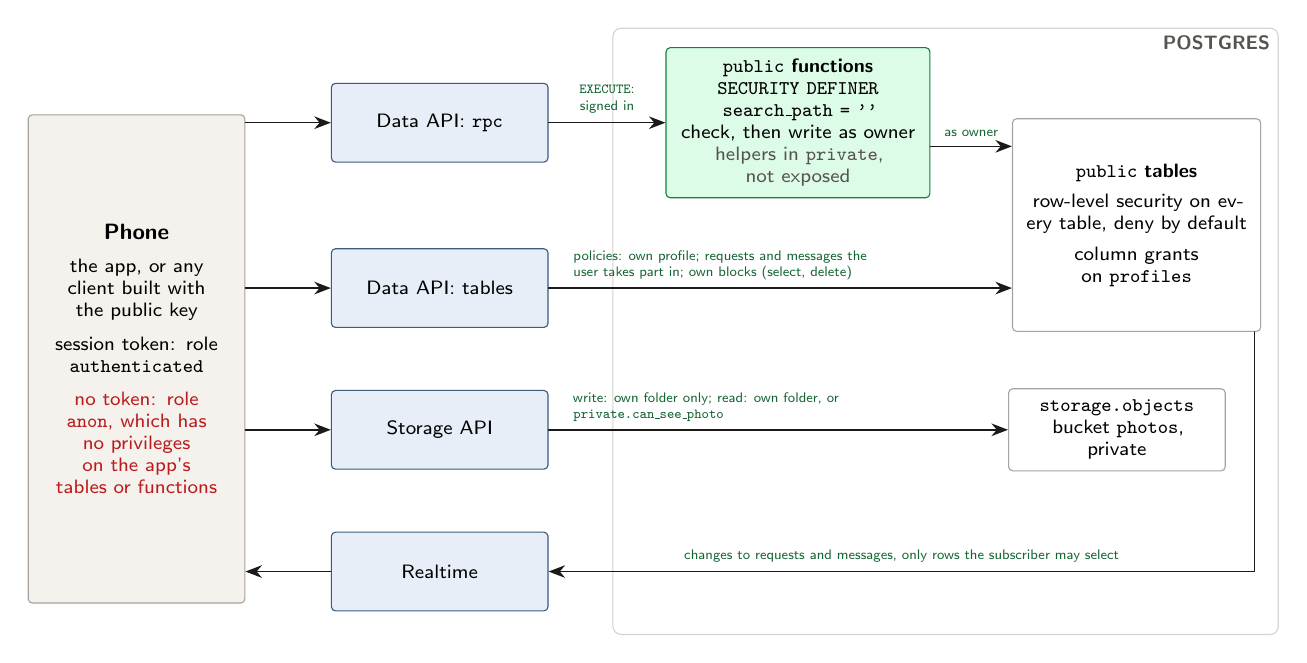
\begin{tikzpicture}[
    svc/.style={box, serverbox, font=\sffamily\scriptsize, text width=24mm, minimum height=10mm, align=center},
    dbbox/.style={box, font=\sffamily\scriptsize, align=center},
    gate/.style={font=\sffamily\tiny, text=accentdark, inner sep=1.2pt, align=center},
  ]
  \node[box, clientbox, font=\sffamily\scriptsize, text width=24mm, minimum height=62mm, align=center] (phone) at (1.25,-2.5)
    {\textbf{\footnotesize Phone}\\[4pt]the app, or any client built with the public key\\[4pt]session token: role \texttt{authenticated}\\[4pt]{\color{alert}no token: role \texttt{anon}, which has no privileges on the app's tables or functions}};

  \node[svc] (rpc) at (5.1,0.5) {Data API: \texttt{rpc}};
  \node[svc] (rest) at (5.1,-1.6) {Data API: tables};
  \node[svc] (storage) at (5.1,-3.4) {Storage API};
  \node[svc] (rt) at (5.1,-5.2) {Realtime};

  \begin{scope}[on background layer]
    \node[layer, fit={(7.3,1.7) (15.75,-6.0)}, inner sep=0pt] (db) {};
  \end{scope}
  \node[layerlabel, anchor=north east] at (db.north east) {POSTGRES};

  \node[dbbox, accentbox, text width=30mm] (fns) at (9.65,0.5) {\textbf{\texttt{public} functions}\\\texttt{SECURITY DEFINER}\\\texttt{search\_path = ''}\\check, then write as owner\\{\color{muted}helpers in \texttt{private}, not exposed}};
  \node[dbbox, text width=28mm, minimum height=27mm] (tables) at (13.95,-0.8) {\textbf{\texttt{public} tables}\\[3pt]row-level security on every table, deny by default\\[3pt]column grants on \texttt{profiles}};
  \node[dbbox, text width=24mm] (objects) at (13.7,-3.4) {\textbf{\texttt{storage.objects}}\\bucket \texttt{photos}, private};

  \foreach \s in {rpc, rest, storage} {\draw[flow] (phone.east |- \s) -- (\s);}
  \draw[flow] (rt) -- (phone.east |- rt);

  \draw[flow] (rpc) -- node[gate, above=2pt] {\texttt{EXECUTE}:\\signed in} (fns);
  \draw[flow] (fns.east |- 0,0.2) -- node[gate, above=2pt] {as owner} (tables.west |- 0,0.2);
  \draw[flow] (rest) -- (tables.west |- rest);
  \node[gate, anchor=south west, text width=40mm, align=flush left] at (6.75,-1.55) {policies: own profile; requests and messages the user takes part in; own blocks (select, delete)};
  \draw[flow] (storage) -- (objects);
  \node[gate, anchor=south west, text width=44mm, align=flush left] at (6.75,-3.35) {write: own folder only; read: own folder, or \texttt{private.can\_see\_photo}};
  \draw[flow] (15.45,0 |- tables.south) -- (15.45,-5.2) -- node[gate, above=2pt] {changes to requests and messages, only rows the subscriber may select} (rt.east);
\end{tikzpicture}

  \caption{Security boundaries. Writes go through functions that check before they act; direct table and
    storage access is limited by policies; Realtime delivers only rows the subscriber could select.}
  \label{fig:security}
\end{figure}

\section{Trust model}

The server trusts nothing the client says about identity or state. The app's address and publishable
key are in the app bundle and must be assumed public, so anyone can build a client that calls the same
API with a valid user session. Every rule therefore lives in the database, where such a client cannot
bypass it:

\begin{itemize}
  \item Identity comes only from the session token, through \code{auth.uid()}.
  \item State, such as whether a user is live, chatting or waiting on a request, is read from the
    database, never taken from arguments.
  \item Proximity is computed from stored positions, never from a distance the client supplies.
  \item Every write passes through a database function, except three the policies confine to the user's
    own data: the profile's client-writable columns, deleting one's own \code{blocks} rows (unblocking),
    and photo files in one's own Storage folder. Each function checks what its action needs; blocks and
    rate limits apply where \cref{tab:functions} lists them, so \code{update_note}, \code{leave_event}
    and \code{end_chat}, for example, check neither.
\end{itemize}

The server must accept two inputs it cannot verify: the position the phone reports, and the GPS accuracy,
which widens the nearby radius by at most 50 metres. The relocation limits bound how a live position may
change (\cref{sec:relocation-limits}); the position sent to join an event is checked only against the
event's distance.

\section{Authentication and sessions}

Accounts are Supabase Auth users with an email address and a password of at least eight characters.
Every new address is confirmed with an emailed 8-digit code before the account can sign in, and a
forgotten password is reset with another emailed code. Supabase limits how often codes are sent; the app
reports those limits as sentences, except when creating an account, which looks the same whether or not
the email already has an account (\cref{sec:flow-account}).

The Supabase client keeps the session in AsyncStorage, refreshes its access token automatically, and does
not look for sessions in URLs. AsyncStorage is used rather than the platform's secure store because the
session JSON is larger than the roughly 2\,KB a secure-store entry holds. Before joining any Realtime
channel the client passes the current token to Realtime, so every channel joins as the signed-in user and
receives only the rows that user may read. On sign-out the app closes every channel, forgets every
signed URL and clears the photos cached on the phone, so the next account to sign in on the same phone
sees nothing of the last one.

\section{Row-level security and grants}
\label{sec:rls}

Row-level security is enabled on every application table and on the three private tables,
\code{private.location_changes}, \code{private.event_posts} and \code{private.blocked_words}. The
anonymous role has no access to any of the app's tables and cannot call any of its functions. \Cref{tab:rls} lists what a
signed-in user may do directly; everything else happens inside a database function.

\begin{table}[ht]
  \centering
  \caption{Direct access for signed-in users. A dash means no access.}
  \label{tab:rls}
  \tablefont
  \begin{tabularx}{\textwidth}{@{}L{28mm}L{34mm}L{30mm}Y@{}}
    \toprule
    \textsf{\textbf{Table}} & \textsf{\textbf{Select}} & \textsf{\textbf{Insert, update}} & \textsf{\textbf{Delete}} \\
    \midrule
    \code{profiles} & own row & own row; editable columns only; \code{is_adult} must be true on insert & --- \\
    \code{availability} & --- & --- & --- \\
    \code{chat_requests} & rows the user sent or received & --- & --- \\
    \code{messages} & chats the user is in and events the user has joined, minus senders the user blocked & --- & --- \\
    \code{events}, \code{event_members} & --- & --- & --- \\
    \code{blocks} & blocks the user made & --- & blocks the user made \\
    \code{reports} & --- & --- & --- \\
    \code{location_changes}, \code{event_posts}, \code{blocked_words} & --- & --- & --- \\
    \code{storage.objects} (\code{photos}) & own folder, or a photo of someone the user can see & directly in own folder, at most 24 files & own folder \\
    \bottomrule
  \end{tabularx}
\end{table}

Column grants close a gap that row-level security alone would leave: a user may update their own profile
row, but only its editable columns. \code{verified} and \code{status} cannot be written by any client, and
\code{id} and \code{is_adult} cannot be changed after the row is created.

Every function is hardened in the same way. \code{SECURITY DEFINER} functions set an empty
\code{search_path}, so a caller cannot make them resolve a name to an object of the caller's choosing.
Execution is revoked from \code{public} and \code{anon}. Helpers live in a schema the Data API does not
expose. A platform helper that Supabase installs, \code{public.rls_auto_enable}, is also revoked from
every API role, because a \code{SECURITY DEFINER} function should not be callable by them even when it
can do nothing outside its intended trigger.

\section{What the functions enforce}

\Cref{tab:functions} lists every check. They fall into seven groups:

\begin{description}
  \item[Identity.] Every function acts as \code{auth.uid()}; a user cannot request, block or report
    themselves.
  \item[Profile standing.] Going live, creating and joining events require an active adult profile;
    only active users can be found or sent a request.
  \item[State.] A request can be answered only while it is \code{pending} and addressed to the caller; a
    chat can be ended or written to only while it is \code{accepted} and the caller takes part in it;
    one request may wait per sender and one chat may run per user; only its host can delete an event.
  \item[Proximity.] Nearby lists and requests require both users to be live within 100 to 150 metres,
    and so does seeing a stranger's photos; joining an event requires being within 5 kilometres of it.
  \item[Blocks.] Any block between two users, in either direction, stops every interaction between
    them (\cref{sec:blocking-reporting}).
  \item[Limits.] Lengths, durations, start times and rates (\cref{tab:rate-limits}).
  \item[Content.] Typed text must show something and carry no control characters, direction overrides or
    piles of accents (check constraints), and text other people see may not contain a word from the word
    filter's list (\cref{sec:word-filter}).
\end{description}

\section{Location privacy}
\label{sec:location-privacy}

\subsection{How a position is handled}

A live position follows a short, fixed path:

\begin{enumerate}
  \item The app asks for \emph{while using the app} permission only, never background location. It reads a
    position when the user taps \ui{Go live} or \ui{Join}, and when the \ui{Map} tab centres on the user. It
    does not follow the user's movements.
  \item \code{go_green} stores the position in the user's \code{availability} row, which no client can read.
  \item Database functions use the position only to compare distances. No function returns it, and no
    function returns a distance: \code{nearby} returns person cards, and the cards contain no location.
  \item \code{go_offline} deletes the row the moment the user goes offline, and the minute job deletes it
    when the session ends. No copy is kept. \code{private.location_changes} keeps the time of each
    location change for ten minutes, but never the place.
\end{enumerate}

The positions sent to \code{events_near} (the centre of the map, usually the user's position) and to
\code{join_event} are used for one query each and are not stored. Event locations
are the exception to all of this by design: they are places hosts choose to publish, and the map shows
them to anyone within the chosen radius.

The nearby radius is deliberately coarse. A user appears to others only as ``nearby'', within 100 metres
plus the viewer's reported accuracy and never beyond 150 metres, and moves of 150 metres or less do not
change the stored position at all (\cref{sec:relocation-limits}), so the list cannot be used to track
someone's small movements.

\subsection{Relocation limits}
\label{sec:relocation-limits}

A modified client could call \code{go_green} with arbitrary coordinates and then \code{nearby}, and so
learn who is live at places the user is not. \code{go_green} limits this probing in three ways:

\begin{itemize}
  \item \textbf{GPS wobble is ignored.} If the user is live and the new position is within 150 metres of
    the stored one, the stored position and its time stay as they were. Small steps therefore cannot add
    up to a large move.
  \item \textbf{Speed.} While the user is live, a larger move must not exceed 150 metres plus walking pace,
    10 km/h, over the time since the stored position was set (\cref{lst:speed}).
  \item \textbf{Frequency.} Starting a session, or moving more than 150 metres, counts as a location
    change. At most three are allowed in any ten minutes.
\end{itemize}

\begin{lstlisting}[language=pgsql, caption={The speed check in \code{go_green}. \code{moved_m} is the distance from the stored position.}, label={lst:speed}]
-- 10 km/h is 10000 m per 3600 s, counted from when your live position was set
allowed_m := 150 + 10000.0 / 3600 * extract(epoch from now() - previous.started_at);
if moved_m > allowed_m then raise exception 'moving too fast'; end if;
\end{lstlisting}

\subsection{The delete-on-offline trade-off}
\label{sec:trade-off}

The go-live screen promises that the location is deleted when the user stops. Keeping that promise means
the server holds no position once a user is offline, and so the speed check can apply only within one
live session. A modified client can therefore go offline, go live somewhere else, and repeat, limited only
by the frequency rule: three location changes in ten minutes, or about eighteen an hour. The alternative,
keeping each user's last position after they go offline so that the speed rule could span sessions, would
have broken the promise. The project chose to keep the promise and accept this residual risk; no cooldown
was added.

\section{Photo privacy}
\label{sec:photo-privacy}

Photos are the most identifying data in Yap, and their protection has four layers.

\paragraph{A private bucket} The \code{photos} bucket is private, so no photo has a public address.
Clients see a photo only through a signed URL, valid for one hour.

\paragraph{Own folder only} Storage policies let a user upload, overwrite and delete only inside the
folder named after their own user ID. Check constraints on \code{profiles} require the profile picture and
every further photo to be a file directly inside the owner's folder, with no deeper path and no
\code{..}, and allow at most six further photos. A profile therefore cannot show someone else's face.

\paragraph{Visible people only} Reading an object, which signing a URL and listing a folder both require,
is allowed for the user's own folder and otherwise only when \code{private.can_see_photo} agrees. It
allows a photo only if all of the following hold:

\begin{itemize}
  \item the file is on the owner's current profile (the profile picture, its 320-pixel copy, or one of
    the further photos), never an older file left in the folder;
  \item neither user has blocked the other;
  \item and one of these is true: the owner is on the user's nearby list right now (owner active, live and
    open, and both near each other); a request between them is waiting, or they are chatting or met; or
    the file is the owner's profile picture and the owner hosts an event the map shows.
\end{itemize}

\paragraph{Short-lived URLs} The policy is checked when a URL is signed. A URL signed while its owner was
visible stays usable until it expires, at most one hour later, even if the owner stops being visible in
the meantime.

\section{What other users can see}

\Cref{tab:exposure} sets out what another user can learn about a person, and when.

\begin{table}[ht]
  \centering
  \caption{What other users can see.}
  \label{tab:exposure}
  \tablefont
  \begin{tabularx}{\textwidth}{@{}L{42mm}Y@{}}
    \toprule
    \textsf{\textbf{Data}} & \textsf{\textbf{Visible to others}} \\
    \midrule
    First name, last initial & On the person card, in event cards (host) and with every message sent \\
    Last name, email address & Never \\
    Gender & On the person card, only if the owner chose to show it and did not choose \ui{Prefer not to say} \\
    Introduction, interests & On the person card \\
    Photos & Through signed URLs, only while the owner is visible to the viewer (\cref{sec:photo-privacy}) \\
    Live note & On the person card while the owner is live; through \code{request_person} only while the request or chat is still going \\
    Live position, distance & Never \\
    Event location & To anyone whose map radius covers it, by design \\
    Being live & Only to other live users nearby, and only while the owner is \code{open} \\
    Blocks and reports & Never; a reported user is not told who reported them \\
    \bottomrule
  \end{tabularx}
\end{table}

The 18+ confirmation is the user's own declaration; the app does not verify age. \code{verified} is
reserved for the selfie check, which is switched off (\cref{sec:feature-flags}).

\section{Blocking and reporting}
\label{sec:blocking-reporting}

A block is stored as one directed row but enforced in both directions. The helper
\code{private.blocked_between} is checked by \code{nearby}, \code{send_request}, \code{request_person},
\code{send_chat_message}, \code{events_near}, \code{join_event} and \code{can_see_photo}, so once either
user blocks the other they no longer appear to each other, cannot send each other requests or chat
messages, cannot load each other's photos, and do not see each other's events. \code{block_user} also
cancels any waiting request and any chat between the two at once. Event group chats are shared spaces: a
blocked user can still write in an event both have joined, but the user who blocked them does not receive
those messages, because the \code{messages} select policy removes them, and the app filters them again.
Unblocking deletes the row, and the person can appear again at the next refresh.

A report records the reason and details. When three different users have reported the same profile, the
profile becomes \code{hidden}: it disappears from nearby lists, cannot receive requests, and its owner can
no longer go live or create or join events, until the owner reviews it. The owner reviews open reports at
least once every 24 hours, as the app stores require, from the Supabase SQL editor with the queries in
\code{docs/legal/moderation.md}, and records each outcome in \code{reviewed_at} and \code{action}. A
profile that broke the guidelines is suspended with \code{private.suspend_user}, which also ends
everything the person is part of (\cref{sec:moderation}); a hidden profile found harmless is set back to
\code{active}. There is no moderator screen in the app. The community guidelines, which every user agrees
to at sign-up, say what is not allowed and that reports are reviewed within 24 hours.

\section{Rate limits and abuse controls}

\Cref{tab:rate-limits} collects the limits that bound what one account can do.

\begin{table}[ht]
  \centering
  \caption{Rate limits.}
  \label{tab:rate-limits}
  \tablefont
  \begin{tabularx}{\textwidth}{@{}L{44mm}L{48mm}Y@{}}
    \toprule
    \textsf{\textbf{Action}} & \textsf{\textbf{Limit}} & \textsf{\textbf{Enforced by}} \\
    \midrule
    Sending requests & 5 per sender in any 10 minutes & \code{send_request} \\
    Waiting requests & 1 per sender at a time & \code{send_request}; partial unique index \\
    Sending messages & 30 per sender per minute, both chat kinds & \code{send_chat_message}, \code{send_event_message} \\
    Creating events & 5 per host in any 24 hours, deleted events included; exact for calls sent at once & \code{create_event} (a per-host lock); \code{private.event_posts} \\
    Reporting & 1 report per person per day; 10 people per day; exact for calls sent at once & \code{report_user} (a per-reporter lock) \\
    Storing photos & 24 files per user; best-effort, as uploads sent at once can go a little past it & storage insert policy \\
    Changing location & 3 changes in any 10 minutes & \code{go_green} \\
    Moving while live & 150\,m plus 10\,km/h since the position was set & \code{go_green} \\
    Email codes & 1 per address per minute on the hosted project; 1 per second on the local stack & Supabase Auth: a dashboard setting; \code{max_frequency} in \code{supabase/config.toml} \\
    Auth requests & Supabase's per-project limits & Supabase Auth \\
    \bottomrule
  \end{tabularx}
\end{table}

\section{Keys and secrets}

The app contains two configuration values, the project URL and the publishable key, both in
\code{src/config/supabase.ts}. Both are public by design: the key grants only what row-level security and
the database functions allow. No secret key, service-role key or SMTP credential is in the repository or
the app; they exist only in the Supabase dashboard. The Android build adds a third value, the Google Maps
key, which ships inside the Android app and is restricted in Google Cloud to the app's package and signing
certificate; it is kept out of the repository as an EAS environment variable.

\chapter{Reliability}
\label{ch:reliability}

A phone is an unreliable place to run a real-time app. The network drops and returns, the operating
system suspends apps in the background, Realtime connections break and rejoin, and the user may close the
app at any moment. This chapter describes how Yap stays correct under those conditions. The guiding rule
is that the server is the source of truth: the client may fall behind, but it always has a way to ask the
server where things stand and catch up.

\section{Failure model}

The design assumes five kinds of failure:

\begin{itemize}
  \item \textbf{Lost Realtime events.} Realtime does not replay changes sent while a channel was
    disconnected, so any event can be missed.
  \item \textbf{Background suspension.} Without push notifications, an app in the background receives
    nothing.
  \item \textbf{Network loss.} Any call can fail, including a call whose effect matters to someone else,
    such as going offline.
  \item \textbf{Restart.} The app can be closed while live, waiting for an answer or in a chat.
  \item \textbf{Races.} Two users can act on the same request at the same moment, and slow answers can
    arrive after newer ones.
\end{itemize}

\section{Realtime subscriptions}
\label{sec:realtime}

The client opens at most three Realtime channels of its own and one per waiting request
(\cref{fig:realtime}). Each is created by the API layer and subscribed through \code{subscribeAsMe}, which
first passes the user's current token to Realtime. Without that step, a session created by some sign-in
paths (the password-reset code, for one) would join channels without the user's token; the database would
then refuse the filter and nothing would arrive. Every subscription accepts an \code{onSubscribed}
callback that runs on the first join and again after every reconnect, which is the moment to fetch
whatever may have been missed.

\begin{figure}[ht]
  \centering
  % Realtime channel map: from table changes to store state (Figure: realtime map).
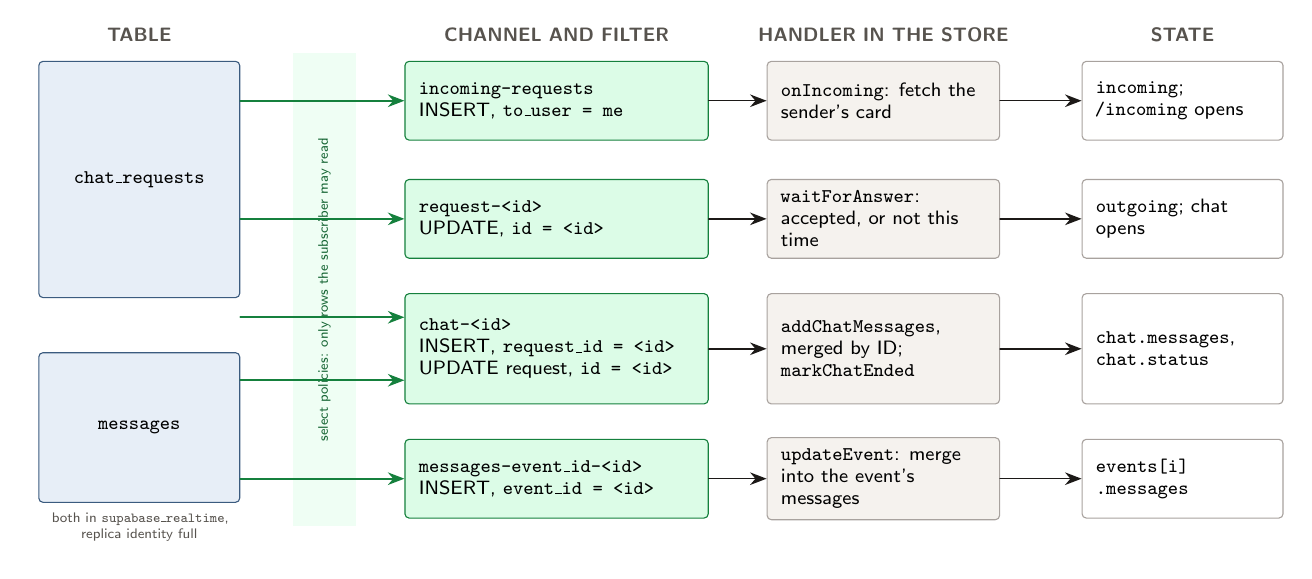
\begin{tikzpicture}[
    tbl/.style={box, serverbox, font=\ttfamily\scriptsize, text width=22mm, align=center},
    ch/.style={box, accentbox, font=\sffamily\scriptsize, text width=35mm, align=flush left, minimum height=10mm},
    hd/.style={box, clientbox, font=\sffamily\scriptsize, text width=26mm, align=flush left, minimum height=10mm},
    st/.style={box, font=\sffamily\scriptsize, text width=22mm, align=flush left, minimum height=10mm},
    lab/.style={font=\sffamily\tiny, text=muted, fill=white, inner sep=1pt},
  ]
  \foreach \x/\t in {1.3/TABLE, 6.6/CHANNEL AND FILTER, 10.75/HANDLER IN THE STORE, 14.55/STATE} {
    \node[layerlabel, anchor=south, inner sep=0pt] at (\x,0.75) {\t};}

  \node[tbl, minimum height=30mm] (req) at (1.3,-1.0) {chat\_requests};
  \node[tbl, minimum height=19mm] (msg) at (1.3,-4.15) {messages};
  \node[font=\sffamily\tiny, text=muted, align=center, text width=26mm, anchor=north] at (msg.south) {both in \texttt{supabase\_realtime}, replica identity full};

  \begin{scope}[on background layer]
    \fill[accentsoft!45] (3.25,0.6) rectangle (4.05,-5.4);
  \end{scope}
  \node[font=\sffamily\tiny, text=accentdark, rotate=90, align=center] at (3.65,-2.4) {select policies: only rows the subscriber may read};

  \node[ch] (c1) at (6.6,0) {\texttt{incoming-requests}\\INSERT, \texttt{to\_user = me}};
  \node[ch] (c2) at (6.6,-1.5) {\texttt{request-<id>}\\UPDATE, \texttt{id = <id>}};
  \node[ch, minimum height=14mm] (c3) at (6.6,-3.15) {\texttt{chat-<id>}\\INSERT, \texttt{request\_id = <id>}\\UPDATE request, \texttt{id = <id>}};
  \node[ch] (c4) at (6.6,-4.8) {\texttt{messages-event\_id-<id>}\\INSERT, \texttt{event\_id = <id>}};

  \node[hd] (h1) at (10.75,0) {\texttt{onIncoming}: fetch the sender's card};
  \node[hd] (h2) at (10.75,-1.5) {\texttt{waitForAnswer}: accepted, or not this time};
  \node[hd, minimum height=14mm] (h3) at (10.75,-3.15) {\texttt{addChatMessages}, merged by ID; \texttt{markChatEnded}};
  \node[hd] (h4) at (10.75,-4.8) {\texttt{updateEvent}: merge into the event's messages};

  \node[st] (s1) at (14.55,0) {\texttt{incoming}; \texttt{/incoming} opens};
  \node[st] (s2) at (14.55,-1.5) {\texttt{outgoing}; chat opens};
  \node[st, minimum height=14mm] (s3) at (14.55,-3.15) {\texttt{chat.messages}, \texttt{chat.status}};
  \node[st] (s4) at (14.55,-4.8) {\texttt{events[i]} \texttt{.messages}};

  \draw[push] (req.east |- c1) -- (c1);
  \draw[push] (req.east |- c2) -- (c2);
  \draw[push] (req.east |- 0,-2.75) -- (c3.west |- 0,-2.75);
  \draw[push] (msg.east |- 0,-3.55) -- (c3.west |- 0,-3.55);
  \draw[push] (msg.east |- c4) -- (c4);
  \foreach \i in {1,2,3,4} {\draw[flow] (c\i) -- (h\i); \draw[flow] (h\i) -- (s\i);}
\end{tikzpicture}

  \caption{Realtime channel map. Two published tables feed four channels; select policies decide which rows
    each subscriber receives; each channel's handler updates one part of the store.
    \Cref{tab:subscriptions} gives when each channel opens and closes.}
  \label{fig:realtime}
\end{figure}

The store keeps exactly one of each of its channels and closes all of them on sign-out. Opening a new
one-to-one chat or group chat closes the previous one first, so a channel is never leaked.

\section{Catch-up}
\label{sec:catch-up}

Because events can be missed, the store has a single procedure, \code{catchUp}, that asks the server
directly where things stand. It runs when the app returns to the foreground, when the network returns,
when the incoming-requests channel re-joins after a disconnection, and when Auth refreshes the token after
a failed load (\cref{fig:catch-up}). Calls never overlap: a call that arrives while one is running makes
it run once more when it finishes.

\begin{figure}[ht]
  \centering
  % The catch-up that runs when the app returns, reconnects or a channel re-joins (Figure: catch-up).
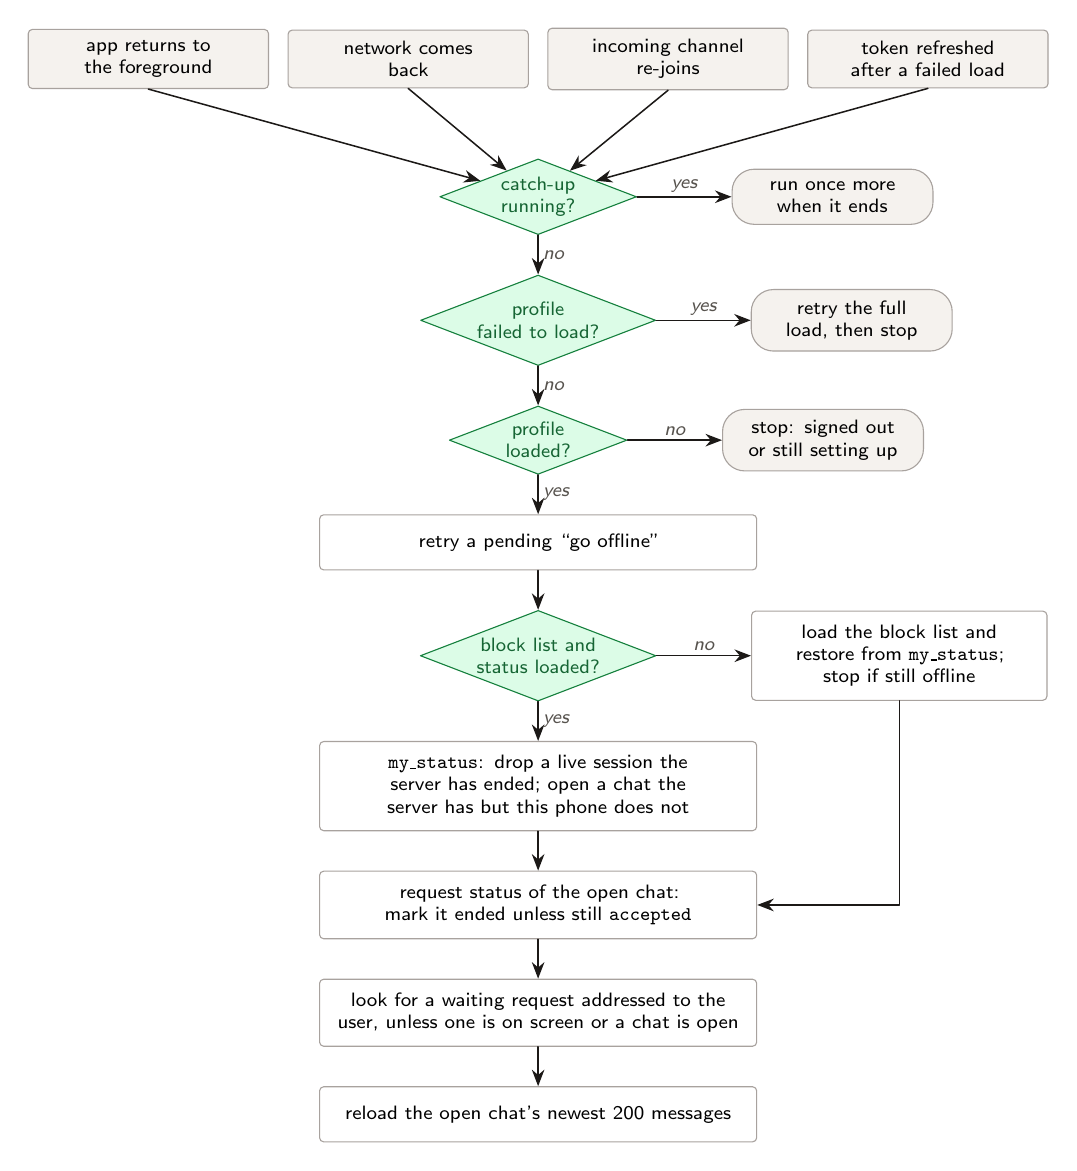
\begin{tikzpicture}[
    node distance=5mm and 8mm,
    st/.style={step=52mm, font=\sffamily\scriptsize},
    trig/.style={box, clientbox, font=\sffamily\scriptsize, text width=27mm, align=center},
    yes/.style={edgelabel, fill=none, font=\sffamily\scriptsize\itshape, text=muted},
    outcome/.style={terminal, font=\sffamily\scriptsize, text width=22mm, align=center},
  ]
  \node[trig] (t1) at (0,0) {app returns to\\the foreground};
  \node[trig] (t2) at (3.3,0) {network comes\\back};
  \node[trig] (t3) at (6.6,0) {incoming channel\\re-joins};
  \node[trig] (t4) at (9.9,0) {token refreshed\\after a failed load};

  \node[decision, aspect=2.6] (running) at (4.95,-1.75) {catch-up\\running?};
  \node[outcome, right=12mm of running] (again) {run once more\\when it ends};
  \node[decision, aspect=2.6, below=of running] (failed) {profile\\failed to load?};
  \node[outcome, right=12mm of failed] (reload) {retry the full\\load, then stop};
  \node[decision, aspect=2.6, below=of failed] (profile) {profile\\loaded?};
  \node[outcome, right=12mm of profile] (stop) {stop: signed out\\or still setting up};
  \node[st, below=of profile] (offline) {retry a pending ``go offline''};
  \node[decision, aspect=2.6, below=of offline] (extras) {block list and\\status loaded?};
  \node[st, text width=34mm, right=12mm of extras] (load) {load the block list and restore from \texttt{my\_status}; stop if still offline};
  \node[st, below=of extras] (status) {\texttt{my\_status}: drop a live session the server has ended; open a chat the server has but this phone does not};
  \node[st, below=of status] (chatcheck) {request status of the open chat: mark it ended unless still \texttt{accepted}};
  \node[st, below=of chatcheck] (incoming) {look for a waiting request addressed to the user, unless one is on screen or a chat is open};
  \node[st, below=of incoming] (sync) {reload the open chat's newest 200 messages};

  \foreach \t in {t1, t2, t3, t4} {\draw[flow] (\t.south) -- (running);}
  \draw[flow] (running) -- node[yes, above] {yes} (again);
  \draw[flow] (running) -- node[yes, right] {no} (failed);
  \draw[flow] (failed) -- node[yes, above] {yes} (reload);
  \draw[flow] (failed) -- node[yes, right] {no} (profile);
  \draw[flow] (profile) -- node[yes, above] {no} (stop);
  \draw[flow] (profile) -- node[yes, right] {yes} (offline);
  \draw[flow] (offline) -- (extras);
  \draw[flow] (extras) -- node[yes, right] {yes} (status);
  \draw[flow] (extras) -- node[yes, above] {no} (load);
  \draw[flow] (status) -- (chatcheck);
  \draw[flow] (load.south) |- (chatcheck.east);
  \draw[flow] (chatcheck) -- (incoming);
  \draw[flow] (incoming) -- (sync);
\end{tikzpicture}

  \caption{The catch-up. Each step tolerates failure; whatever fails is tried again by the next
    catch-up.}
  \label{fig:catch-up}
\end{figure}

Each step repairs one kind of drift between the phone and the server:

\begin{itemize}
  \item A pending request to go offline is sent again (\cref{sec:offline}).
  \item If the profile has not loaded, because the user is signed out or still setting up, the catch-up
    stops here. If the block list and status never loaded, they are loaded now instead of the next step.
  \item \code{my_status} reveals a live session the server has ended while the app was asleep; the app
    then shows \ui{Your time's up}. It also reveals a chat that was accepted just before the connection
    dropped.
  \item A query of the open chat's request status (\code{api.requestStatus}) reveals a chat the other
    user ended or deleted with their account: anything other than \code{accepted} marks it ended.
  \item A query for the newest waiting request addressed to the user finds a request that arrived while
    the app was in the background.
  \item The open chat's history is reloaded and merged by message ID.
\end{itemize}

The catch-up never undoes something the user did while it was running. It drops the live session only if
the session on the phone is the same object it was before the call, so a fresh \ui{Go live} is not
cancelled by a stale answer, and it opens a chat only if no chat changed on the phone in the meantime.

\section{Offline behaviour}
\label{sec:offline}

\Cref{tab:offline} lists how each action behaves without a connection. A banner tells the user the phone
is offline whenever the operating system reports no connection or no internet.

\begingroup\tablefont
\begin{longtable}{@{}L{46mm}L{\dimexpr\linewidth-46mm-2\tabcolsep\relax}@{}}
  \caption{Behaviour without a connection.}
  \label{tab:offline}\\
  \toprule
  \textsf{\textbf{Situation}} & \textsf{\textbf{Behaviour}} \\
  \midrule
  \endfirsthead
  \toprule
  \textsf{\textbf{Situation}} & \textsf{\textbf{Behaviour}} \\
  \midrule
  \endhead
  \bottomrule
  \endfoot
  Launch with a stored session & The profile cannot load, so \ui{Can't reach Yap} replaces the app, with \ui{Try again}; the load is retried when the token refreshes or a catch-up runs \\
  Go live, say hi, accept, send a message, create, join or delete an event & The call fails and an alert explains; nothing changes on the server. A failed \ui{Accept} also closes the request screen, and the request later expires \\
  Go offline by tapping the red button & The phone shows the user offline at once; \ui{Almost offline} appears, and the call is retried at the next catch-up \\
  Live session reaches its end time & The phone shows the user offline; the server's minute job removes the session on time anyway \\
  Nearby refresh & The last list stays on screen \\
  Waiting for an answer & Realtime and the poll fail quietly; the timer shows \ui{Not this time} after the end time; if the request was in fact accepted, the catch-up opens the chat \\
  Chat accepted but not yet opened & An alert says the chat opens as soon as the phone is back online; the catch-up opens it \\
  Messages, requests or a chat ending missed while away & Recovered by the channel re-joining and by the catch-up \\
  Map & The existing pins stay \\
  A person's further photos & The profile shows without them \\
  Sign out & Refused with an explanation, because ending the chat and going offline must reach the server first \\
\end{longtable}
\endgroup

\section{Ordering and races}
\label{sec:ordering}

Several guards keep late or duplicate work from corrupting state.

\paragraph{On the server} \code{respond}, \code{cancel_request} and \code{end_chat} lock the request row
before deciding, so concurrent actions on one request apply in sequence. A partial unique index makes a
second waiting request from one sender impossible even if two calls race. \code{respond} withdraws the
recipient's own waiting request before checking for an existing chat, so an answer landing at the same
moment is seen. A cancel that arrives just after an accept ends the new chat instead of leaving one user
in a chat the other never sees.

\paragraph{Double taps} Every button, icon button, row and card ignores a second tap while the action
the first one started is still running (the button shows its spinner meanwhile), and for half a second
after a tap that only opens or closes a screen (\code{useGuardedPress} in
\code{src/components/ui/press-feedback.ts}), so a double tap cannot submit twice, open a screen twice or go
back two screens. Forms that a keyboard key or a completed code can also submit run one attempt at a time
(\code{useOneAtATime}). The server makes the repeats that still get through harmless: saying hi again to
the person already waited on returns the same request, a repeated report keeps the first, and joining,
blocking and going live again change nothing.

\paragraph{In the store}
\begin{itemize}
  \item A say-hi on its way to the server blocks a second one, and a sign-out or account deletion
    already under way makes a second tap of the same action wait for it. The other action is refused
    with an error rather than waiting, so a sign-out never passes for a deletion.
  \item Sign-out resets every counter and in-flight marker below, so an answer meant for the previous
    account lands nowhere.
  \item Counters on nearby refreshes, event loads and group chat visits discard any answer that arrives
    after a newer request has started or the screen has closed.
  \item \code{handledRequestIds} and \code{closedChatIds} stop a catch-up, which may have read the server a
    moment earlier, from reviving a request already answered or a chat already closed on this phone.
  \item \code{openingChatId} stops the same chat being opened twice when Realtime and a catch-up report it
    together.
  \item Chats subscribe before loading history and merge messages by ID, so no message is lost between
    the two steps and none is shown twice.
  \item Going live waits for an in-flight retry of going offline, so the retry cannot delete the new
    session.
  \item \code{init()} runs once per process, however often the root layout mounts.
\end{itemize}

\section{Time}
\label{sec:time}

The server owns every deadline. \code{go_green} returns the session's start and end as the server set
them, and \code{send_request} returns the request's end time; the countdowns on screen count towards those
instants. A phone's clock can be wrong, set by hand or minutes off, so the app does not compare those
instants with the phone's clock directly. \code{my_status} also returns the server's clock, and each time
it is called (at launch and at every catch-up) the app records how far the phone's clock is off, taking
the server's answer as halfway through the round trip (\code{src/lib/server-clock.ts}).
\code{serverNow()}, the phone's clock corrected by that offset, drives the shared countdown clock, the
end-of-session timer, the wait for an answer, the query for missed requests and the earliest start of a
new event. Before the first answer the offset is zero, which was the behaviour before. Whatever the
phone's clock says, it cannot extend a session or a request, because the server checks its own time and
its minute job removes whatever has run out.

The countdowns themselves share one clock (\code{useClock}): a single one-second interval serves every
countdown on screen and stops when none is shown. It reads the time outside React's render, as React
requires, and copes with the device clock being changed.

\section{Staying reachable without push notifications}

Yap does not send push notifications, so a request reaches a user only while the app is open. Two choices
follow from that. While the user is live, the app keeps the screen awake, and the \ui{Go live} tab says so
(\ui{Keep Yap open to get requests}). And every screen that a request or a chat opens is a normal route
(\code{/incoming}, \code{/chat}), opened by the \code{(app)} layout, so a push notification added later
can open the same routes.

\section{Error handling}

Errors are handled at the edge where they can be explained. The API layer turns every refusal, Auth error
and network failure into a sentence. Screens catch the errors of the actions they start and show them in
an alert or inline. Store actions catch the failures that are expected while offline and leave them to the
next catch-up. The result is that a user always sees a short explanation, never a stack trace or database
text, and an action that failed can simply be tried again.

\section{Timers and schedules}

\Cref{tab:timers} lists every timer in the system.

\begin{table}[ht]
  \centering
  \caption{Timers and schedules.}
  \label{tab:timers}
  \tablefont
  \begin{tabularx}{\textwidth}{@{}L{48mm}L{40mm}Y@{}}
    \toprule
    \textsf{\textbf{Timer}} & \textsf{\textbf{Period or delay}} & \textsf{\textbf{Owner}} \\
    \midrule
    Housekeeping job & every minute & \code{pg_cron}, \code{expire_stale} \\
    Sign-in record pruning & daily at 03:00 & \code{pg_cron}, \code{prune_audit_log} \\
    Request answer window & 5 minutes & \code{chat_requests.expires_at} \\
    Nearby refresh & every 20\,s, foreground only & \code{useNearbyPolling} \\
    Answer poll & every 7\,s & \code{waitForAnswer} \\
    Answer timer & end time plus 3\,s & \code{waitForAnswer} \\
    End of live session & at the server's end time & \code{(app)/_layout} \\
    Countdown clock & every second, while shown & \code{useClock} \\
    Location fix & up to 8\,s & \code{useForegroundLocation}, map \\
    Nearby prompt & 8\,s on screen & \code{NearbyToast} \\
    Code resend & 60\,s cooldown & \code{(auth)/verify} \\
    Signed photo URL & 15 minutes; reused until 5 minutes remain; refusals retried after 60\,s & \code{signPaths} \\
    \bottomrule
  \end{tabularx}
\end{table}

\chapter{Performance}
\label{ch:performance}

Yap's workload is small per user but frequent: every live user refreshes a nearby list every 20 seconds,
and every list shows photos. The design keeps each refresh to one database query and as few photo
downloads as possible. \Cref{fig:nearby-path} follows one refresh and notes the work saved at each step;
the rest of the chapter lists the choices that matter, grouped by where they act.

\begin{figure}[ht]
  \centering
  % The nearby refresh path and the work saved at each step (Figure: nearby path).
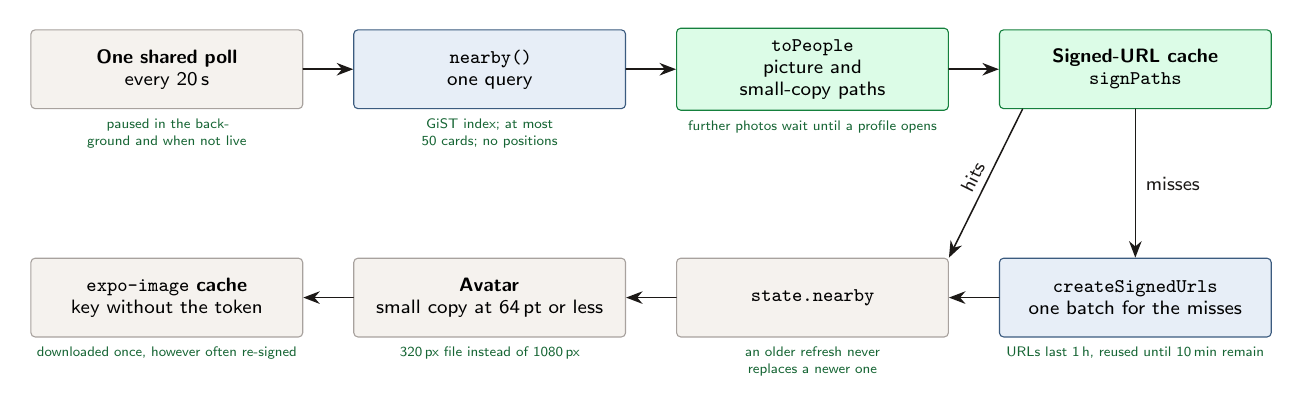
\begin{tikzpicture}[
    stepbox/.style={box, font=\sffamily\scriptsize, text width=31mm, minimum height=10mm, align=center},
    saving/.style={font=\sffamily\tiny, text=accentdark, text width=33mm, align=center, anchor=north},
  ]
  \node[stepbox, clientbox] (poll) at (1.85,0) {\textbf{One shared poll}\\every 20\,s};
  \node[stepbox, serverbox] (rpc) at (5.95,0) {\textbf{\texttt{nearby()}}\\one query};
  \node[stepbox, accentbox] (paths) at (10.05,0) {\textbf{\texttt{toPeople}}\\picture and small-copy paths};
  \node[stepbox, accentbox] (cache) at (14.15,0) {\textbf{Signed-URL cache}\\\texttt{signPaths}};

  \node[stepbox, serverbox] (sign) at (14.15,-2.9) {\textbf{\texttt{createSignedUrls}}\\one batch for the misses};
  \node[stepbox, clientbox] (state) at (10.05,-2.9) {\textbf{\texttt{state.nearby}}};
  \node[stepbox, clientbox] (avatar) at (5.95,-2.9) {\textbf{Avatar}\\small copy at 64\,pt or less};
  \node[stepbox, clientbox] (img) at (1.85,-2.9) {\textbf{\texttt{expo-image} cache}\\key without the token};

  \draw[flow] (poll) -- (rpc);
  \draw[flow] (rpc) -- (paths);
  \draw[flow] (paths) -- (cache);
  \draw[flow] (cache) -- node[edgelabel, right=2pt, fill=none] {misses} (sign);
  \draw[flow] (sign) -- (state);
  \draw[flow] (cache.south west) ++(0.3,0) -- node[edgelabel, fill=none, sloped, above=1pt] {hits} (state.north east);
  \draw[flow] (state) -- (avatar);
  \draw[flow] (avatar) -- (img);

  \node[saving] at (poll.south) {paused in the background and when not live};
  \node[saving] at (rpc.south) {GiST index; at most 50 cards; no positions};
  \node[saving] at (paths.south) {further photos wait until a profile opens};
  \node[saving] at ($(sign.south)+(0,0)$) {URLs last 1\,h, reused until 10\,min remain};
  \node[saving] at (state.south) {an older refresh never replaces a newer one};
  \node[saving] at (avatar.south) {320\,px file instead of 1080\,px};
  \node[saving] at (img.south) {downloaded once, however often re-signed};
\end{tikzpicture}

  \caption{One nearby refresh. Most refreshes end with cache hits: no new signed URLs and no downloads.}
  \label{fig:nearby-path}
\end{figure}

\section{Database}

\begin{description}
  \item[A table of live users only.] \code{availability} holds a row only while its user is live, and
    rows are deleted on going offline and by the minute job. The table that every nearby query scans is
    therefore as small as the number of people live at that moment, whatever the number of accounts.
  \item[Spatial indexes.] \code{availability.location} and \code{events.location} have GiST indexes, so
    the distance tests in \code{nearby}, \code{near_each_other} and \code{events_near} use an index rather
    than a scan.
  \item[Partial indexes.] Indexes restricted to \code{pending} and \code{accepted} requests stay small,
    because at any moment few requests are waiting or open. They serve the one-request and one-chat checks,
    \code{my_status} and the minute job.
  \item[Indexed rate limits.] Each rate limit counts a user's recent rows. The counts for requests,
    messages and location changes use indexes on the user and the time; the count of events created uses
    the index on the host.
  \item[Bounded results.] \code{nearby} and \code{events_near} return at most 50 rows; chat history is the
    newest 200 messages, read through an index on the chat and time.
  \item[Work done in one call.] Person cards and event cards are assembled in the database, so a list
    needs one round trip. \code{my_status} restores the live session, the chat and the waiting request in
    one call. The send functions return the saved message, so the sender does not read it back.
\end{description}

\section{Network}

\begin{description}
  \item[One shared nearby poll.] A single poll in the \code{(app)} layout feeds the list, the person sheet
    and the prompts. It runs only while the user is live and the app is in the foreground.
  \item[Photos signed in batches and cached.] All the photo paths a screen needs are signed in one
    request. Signed URLs are reused until ten minutes before they expire, so the same photo keeps the same
    address across refreshes.
  \item[Downloads cached by stable keys.] \code{expo-image} caches each photo under its URL without the
    signing token, so a photo is downloaded once even when its URL is signed again.
  \item[Small copies for small avatars.] Each profile picture has a 320-pixel copy. Avatars of 64 points
    or less, such as those in lists, prompts and the chat header, use it, and so does the host's photo
    on an event.
  \item[Lazy further photos.] Lists sign only profile pictures. A person's further photos are signed when
    their profile is opened, keyed by their paths so that a nearby refresh does not sign them again.
  \item[Smaller uploads.] Photos are re-encoded on the phone as JPEG at most 1080 pixels wide, at quality
    0.8, and never enlarged. The resize reuses the image already decoded instead of reading the file again.
  \item[Filtered Realtime.] Each channel filters on one column (\code{to_user}, \code{id},
    \code{request_id} or \code{event_id}), so the server sends a client only the rows it subscribed to.
\end{description}

\section{Rendering}

\begin{description}
  \item[Selective re-rendering.] Components subscribe to slices of the store through selectors, so a
    change re-renders only the components whose slice changed. The React Compiler, enabled as an Expo
    experiment, memoises components automatically.
  \item[One clock for all countdowns.] A single one-second interval drives every countdown on screen and
    stops when none is shown.
  \item[Virtualised lists.] The nearby list, the blocked list and both chat threads use \code{FlatList};
    chat threads are inverted, so they open at the newest message without scrolling.
  \item[Static map markers.] Event pins are custom views drawn once (\code{tracksViewChanges} is off), so
    the map does not redraw them on every frame.
  \item[Stable list data.] The nearby refresh replaces the list only when an answer is current, and event
    reloads keep the messages already loaded for each event.
\end{description}

\chapter{Configuration and environments}
\label{ch:configuration}

\section{Environments}

Yap has one backend environment: a hosted Supabase project, which every build of the app uses
(\cref{fig:deployment}). The app reaches it through the URL and publishable key in
\code{src/config/supabase.ts}. There is no separate staging project; behaviour that must be proved
against a database is proved against a disposable local Supabase stack (\cref{ch:testing}).
\Cref{app:config} lists every configuration value.

\begin{figure}[ht]
  \centering
  % Environments and how code and schema reach them (Figure: deployment).
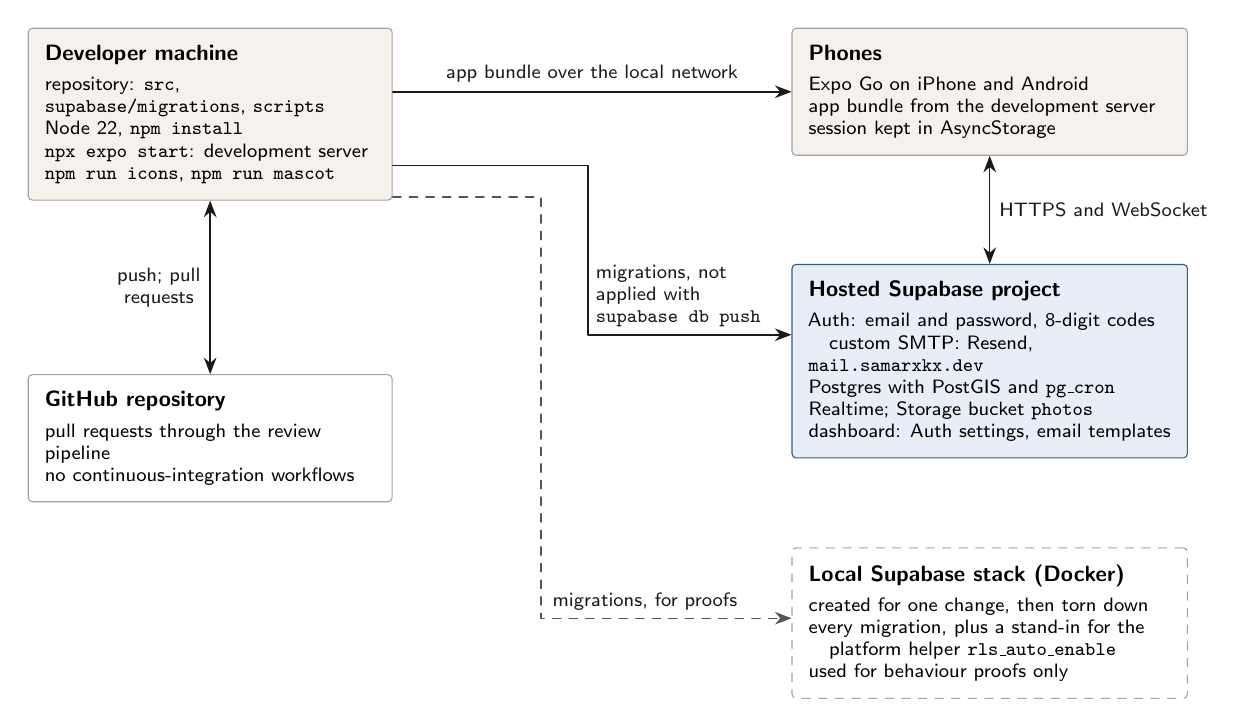
\begin{tikzpicture}[
    env/.style={box, font=\sffamily\scriptsize, align=flush left, inner sep=6pt, anchor=north},
    lab/.style={font=\sffamily\scriptsize, text=ink, fill=white, inner sep=1.2pt, align=center},
  ]
  \node[env, clientbox, text width=42mm] (dev) at (2.4,0)
    {\textbf{\footnotesize Developer machine}\\[3pt]
     repository: \texttt{src}, \texttt{supabase/migrations}, \texttt{scripts}\\
     Node 22, \texttt{npm install}\\
     \texttt{npx expo start}: development server\\
     \texttt{npm run icons}, \texttt{npm run mascot}};
  \node[env, clientbox, text width=46mm] (phones) at (12.3,0)
    {\textbf{\footnotesize Phones}\\[3pt]
     Expo Go on iPhone and Android\\
     app bundle from the development server\\
     session kept in AsyncStorage};
  \node[env, serverbox, text width=46mm] (hosted) at (12.3,-3.0)
    {\textbf{\footnotesize Hosted Supabase project}\\[3pt]
     Auth: email and password, 8-digit codes\\
     \quad custom SMTP: Resend, \texttt{mail.samarxkx.dev}\\
     Postgres with PostGIS and \texttt{pg\_cron}\\
     Realtime; Storage bucket \texttt{photos}\\
     dashboard: Auth settings, email templates};
  \node[env, text width=46mm, dashed] (local) at (12.3,-6.6)
    {\textbf{\footnotesize Local Supabase stack (Docker)}\\[3pt]
     created for one change, then torn down\\
     every migration, plus a stand-in for the\\
     \quad platform helper \texttt{rls\_auto\_enable}\\
     used for behaviour proofs only};
  \node[env, text width=42mm] (gh) at (2.4,-4.4)
    {\textbf{\footnotesize GitHub repository}\\[3pt]
     pull requests through the review pipeline\\
     no continuous-integration workflows};

  \draw[flow] (dev.east |- phones.west) -- node[lab, above=2pt] {app bundle over the local network} (phones.west);
  \draw[flow, <->] (phones.south) -- node[lab, right=2pt] {HTTPS and WebSocket} (hosted.north);
  \draw[flow] (dev.east |- 0,-1.75) -- (7.2,-1.75) |- (hosted.west |- 0,-3.9);
  \node[lab, anchor=south west, align=left, fill=none] at (7.25,-3.85) {migrations, not\\applied with\\\texttt{supabase db push}};
  \draw[softflow] (dev.east |- 0,-2.15) -- (6.6,-2.15) |- (local.west |- 0,-7.5);
  \node[lab, anchor=south west, align=left] at (6.7,-7.45) {migrations, for proofs};
  \draw[flow, <->] (dev.south) -- node[lab, left=2pt] {push; pull\\requests} (gh.north);
\end{tikzpicture}

  \caption{Environments. Phones run the app in Expo Go against the hosted project; migrations reach the
    hosted project from the repository; a throwaway local stack is used only to prove changes.}
  \label{fig:deployment}
\end{figure}

\section{Supabase dashboard settings}
\label{sec:dashboard}

Some configuration lives in the Supabase dashboard rather than in the repository. The README records the
settings that password sign-in needs, and the project's email delivery is configured alongside them
(\cref{tab:dashboard}).

\begin{table}[ht]
  \centering
  \caption{Settings made in the Supabase dashboard.}
  \label{tab:dashboard}
  \tablefont
  \begin{tabularx}{\textwidth}{@{}L{50mm}Y@{}}
    \toprule
    \textsf{\textbf{Setting}} & \textsf{\textbf{Value}} \\
    \midrule
    Auth, email provider & Enabled for password sign-in; \ui{Confirm email} on; minimum password length 8 \\
    Template: confirm sign-up & Shows the 8-digit code (\texttt{\{\{ .Token \}\}}) \\
    Template: reset password & Shows the 8-digit code instead of a link, with a subject such as \ui{Reset your Yap password} \\
    Template: magic link & No longer used by the app \\
    Email delivery & Custom SMTP through Resend, sending from \code{mail.samarxkx.dev} \\
    Apple and Google providers & Not configured; the app's buttons are behind a flag \\
    \bottomrule
  \end{tabularx}
\end{table}

The \code{pg_cron} extension and its schedule, the \code{photos} bucket, the Realtime publication and all
policies are created by the migrations, not by hand.

\section{Database migrations}
\label{sec:migrations}

The schema is defined by eight SQL migrations in \code{supabase/migrations}, listed in
\cref{app:migrations}. Each later migration replaces functions with \code{CREATE OR REPLACE}, which keeps
their grants, or drops and recreates a function whose arguments or return type change and then grants it
again in the same way as the original.

Two practices govern how migrations reach the hosted project. First, the hosted project's recorded
migration versions do not match the file names in the repository, so a new migration is applied in the
same way as the earlier ones rather than with \code{supabase db push}. Second, an app change and the
migration it depends on ship together: after the server-rules migration, for example, \code{join_event}
takes the phone's position, so an older app build can no longer join events.

\code{src/data/database.types.ts} holds TypeScript types generated from the schema, which give the
Supabase client typed tables and function arguments. It is regenerated with
\code{supabase gen types typescript} (or the equivalent Supabase tool) whenever a migration changes tables
or functions.

\section{Local development}

The README describes the development loop:

\begin{lstlisting}[language=bash, caption={Running the app for development.}, label={lst:run}]
nvm use            # Node 22, from .nvmrc
npm install
npx expo start     # scan the QR code with Expo Go on an iPhone or Android phone
\end{lstlisting}

The app runs in Expo Go against the hosted project. Exercising the core loop needs two phones signed in
with different email addresses, within about 100 metres of each other, both live. The native
\code{ios} and \code{android} folders are generated and not committed.

A local Supabase stack can run the migrations for testing, with one adjustment: migration
\code{20261004210004_lock_platform_helper.sql} revokes \code{public.rls_auto_enable()}, a function the
hosted platform installs, so a local stack needs a stand-in for it.

\section{App configuration}

\code{app.json} configures the build (\cref{tab:app-json}).

\begin{table}[ht]
  \centering
  \caption{App configuration in \code{app.json}.}
  \label{tab:app-json}
  \tablefont
  \begin{tabularx}{\textwidth}{@{}L{44mm}Y@{}}
    \toprule
    \textsf{\textbf{Key}} & \textsf{\textbf{Value}} \\
    \midrule
    Name, slug, version & \code{Yap}, \code{yap}, \code{1.0.0}; portrait only; URL scheme \code{yap} \\
    Appearance & \code{automatic}: light or dark from the phone's setting \\
    iOS icon & The \code{assets/expo.icon} bundle, which draws the brand mark over a green fill \\
    Android icon & Adaptive icon with foreground, background and monochrome layers; background \texttt{\#15803D} \\
    Splash screen & Brand mark on \texttt{\#FAF8F5} (light) or \texttt{\#181715} (dark) \\
    Location permission & When in use only, with the text ``Yap uses your location only while you are available, to show you people who are up for a chat in the same place. Nobody sees where you are.'' \\
    Photo and camera permissions & For choosing a profile photo, and for taking one and a verification selfie \\
    Plugins & Expo Router, splash screen, location, image picker, date and time picker \\
    Experiments & Typed routes; React Compiler \\
    \bottomrule
  \end{tabularx}
\end{table}

\section{Feature flags}

Two feature flags in \code{src/config/features.ts} are both off: \code{selfieVerification} and
\code{socialSignIn} (\cref{sec:feature-flags}). Turning a flag on shows the corresponding screens and
buttons; neither feature has a working backend yet.

\section{Asset pipelines and scripts}

Two scripts regenerate assets from source drawings, so the drawings are the single source of truth
(\cref{tab:scripts}).

\begin{description}
  \item[Icons.] \code{npm run icons} runs \code{scripts/make-icons.sh}, which uses ImageMagick 7 to draw
    the brand mark in \code{assets/brand/yap-mark.svg} into the app icon, the three Android adaptive-icon
    layers, the light and dark splash images and the favicon, and copies the SVG into the iOS icon bundle.
    Colours come from the theme tokens. It strips metadata from every image, so re-running it without
    changes leaves the working tree clean.
  \item[Mascot.] \code{npm run mascot} runs \code{scripts/make-mascot.mjs}, which reads each drawing in
    \code{assets/mascot}, removes titles and comments, and writes them as strings into
    \code{src/components/mascot/mascot-art.ts}. Each file name becomes a pose, drawn with
    \code{react-native-svg} without any extra bundler setup.
\end{description}

\begin{table}[ht]
  \centering
  \caption{Package scripts.}
  \label{tab:scripts}
  \tablefont
  \begin{tabularx}{\textwidth}{@{}L{34mm}L{50mm}Y@{}}
    \toprule
    \textsf{\textbf{Script}} & \textsf{\textbf{Command}} & \textsf{\textbf{Purpose}} \\
    \midrule
    \code{start} & \code{expo start} & Development server \\
    \code{ios}, \code{android} & \code{expo start --ios}, \code{--android} & Development server opening a simulator or device \\
    \code{web} & \code{expo start --web} & From the Expo template; the web target is not supported (\cref{ch:limitations}) \\
    \code{lint} & \code{expo lint} & ESLint with the Expo configuration \\
    \code{icons} & \code{sh scripts/make-icons.sh} & Regenerate icons, splash images and favicon \\
    \code{mascot} & \code{node scripts/make-mascot.mjs} & Regenerate the mascot drawings module \\
    \bottomrule
  \end{tabularx}
\end{table}

\chapter{Testing and validation}
\label{ch:testing}

Yap has no client test suite. Correctness is established by static checks and continuous integration on
every change, a small set of SQL tests for the server rules, behaviour proofs run against a disposable
backend for changes that alter behaviour, and manual testing on phones. This chapter describes
each and states plainly what is not covered. \Cref{fig:validation} shows the path a change takes.

\begin{figure}[ht]
  \centering
  % How a change is validated before it reaches main (Figure: validation).
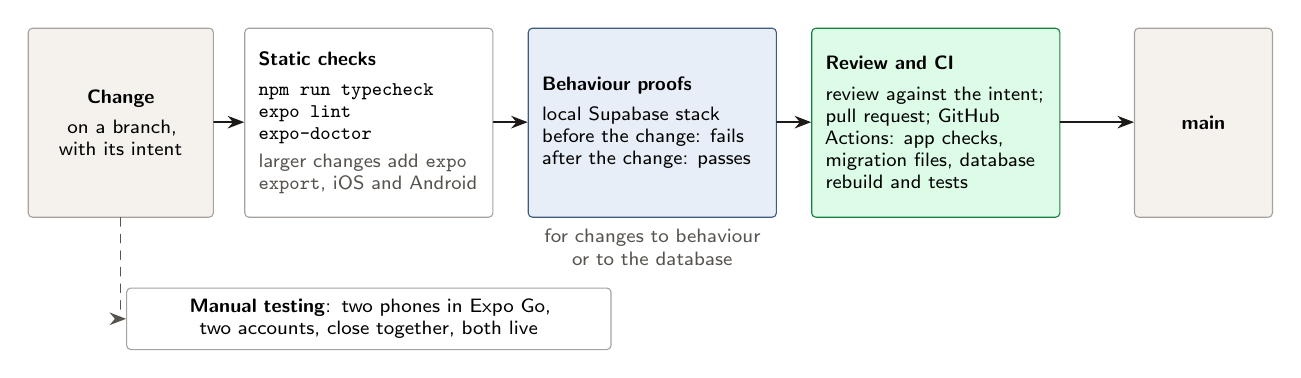
\begin{tikzpicture}[
    stage/.style={box, font=\sffamily\scriptsize, text width=28mm, minimum height=24mm, align=flush left, anchor=north},
    lab/.style={font=\sffamily\scriptsize, text=muted, fill=white, inner sep=1.2pt},
  ]
  \node[stage, clientbox, text width=20mm, align=center] (change) at (1.2,0) {\textbf{Change}\\[3pt]on a branch, with its intent};
  \node[stage] (static) at (4.35,0) {\textbf{Static checks}\\[3pt]\texttt{npm run typecheck}\\\texttt{expo lint}\\\texttt{expo-doctor}\\[2pt]{\color{muted}larger changes add \texttt{expo export}, iOS and Android}};
  \node[stage, serverbox] (proofs) at (7.95,0) {\textbf{Behaviour proofs}\\[3pt]local Supabase stack\\before the change: fails\\after the change: passes};
  \node[stage, accentbox] (pipeline) at (11.55,0) {\textbf{Review and CI}\\[3pt]review against the intent; pull request; GitHub Actions: app checks, migration files, database rebuild and tests};
  \node[stage, clientbox, text width=14mm, align=center] (main) at (14.95,0) {\textbf{main}};

  \draw[flow] (change.east |- 0,-1.2) -- (static.west |- 0,-1.2);
  \draw[flow] (static.east |- 0,-1.2) -- (proofs.west |- 0,-1.2);
  \draw[flow] (proofs.east |- 0,-1.2) -- (pipeline.west |- 0,-1.2);
  \draw[flow] (pipeline.east |- 0,-1.2) -- (main.west |- 0,-1.2);
  \node[lab, anchor=north, text width=32mm, align=center] at ($(proofs.south)+(0,-0.1)$) {for changes to behaviour or to the database};

  \node[box, font=\sffamily\scriptsize, text width=58mm, align=center, anchor=north] (manual) at (4.35,-3.3)
    {\textbf{Manual testing}: two phones in Expo Go, two accounts, close together, both live};
  \draw[softflow] (change.south) |- (manual.west);
\end{tikzpicture}

  \caption{Validation of a change before it reaches \code{main}.}
  \label{fig:validation}
\end{figure}

\section{Static checks}

The README lists three checks, and continuous integration adds a fourth:

\begin{description}
  \item[Type check.] \code{npm run typecheck} type-checks the whole client in TypeScript's strict mode,
    including the typed routes and the database types generated from the schema, so a call with the wrong
    function arguments or a link to a missing route fails to compile. The route types are generated, not
    committed, so the script first writes them to \code{.expo/types} with the command
    \code{expo customize tsconfig.json} and only then runs \code{tsc --noEmit}. Without that step a fresh
    checkout, such as the one in CI, would accept any route string.
  \item[Lint.] \code{npm run lint} runs ESLint with Expo's configuration and the rules of the ESLint
    security plugin, which flag risky patterns such as \code{eval}. A web rule about apostrophes in markup is turned off because it
    does not apply to React Native text, and the security rule that flags every \code{object[key]} is
    turned off because TypeScript already checks those.
  \item[Project health.] \code{npx expo-doctor} checks that the installed packages match the Expo SDK.
  \item[Release bundles.] Exporting with \code{npx expo export}, once with \code{--platform ios} and once
    with \code{--platform android}, builds the production JavaScript bundles and so proves that the app
    bundles for both platforms.
\end{description}

\section{Continuous integration}
\label{sec:ci}

GitHub Actions (\code{.github/workflows/ci.yml}) runs on every pull request and every push to
\code{main}, and a newer push to the same branch cancels the older run. Three jobs report separately:

\begin{description}
  \item[App.] \code{npm ci}, the type check, the lint with warnings treated as failures, \code{expo-doctor}
    and both release bundles, plus an \code{npm audit} report of the production dependencies that never
    fails the run.
  \item[Migration files.] Every migration is named \code{<14-digit version>\_<name>.sql}; a new one must be
    later than every migration on the target branch; and an existing migration that is edited or deleted
    fails the check (\code{scripts/check-migrations.sh}). A rename that leaves the file byte for byte the
    same passes, so a file can take the version the hosted project recorded (\cref{app:migrations}).
  \item[Database (reset, lint, tests, types).] Starts Supabase in Docker with a pinned CLI version, applies
    every migration to an empty database with \code{supabase db reset}, lints the functions in
    \code{public} and \code{private} with \code{supabase db lint}, runs the SQL tests in
    \code{supabase/tests} with \code{supabase test db}, and fails when \code{src/data/database.types.ts}
    differs from the types generated from the migrations (\code{npm run db:types:check}).
\end{description}

Dependabot opens weekly update pull requests for npm packages and GitHub Actions; packages whose version
the Expo SDK decides only move in an SDK upgrade. An optional AI review (PR-Agent, with a Gemini API key)
stays off until the owner turns it on. \code{docs/RELEASING.md} describes the whole flow around these
checks: branches and squash-merged pull requests, the branch protection that should require the three
jobs (not yet switched on), versioning, EAS builds and store submission, applying database changes,
rolling back, dependency updates and the optional review (\cref{sec:release}).

\section{SQL tests}

The pgTAP file \code{supabase/tests/hardening_test.sql} runs against the local stack with
\code{supabase test db}, inside a transaction it rolls back. Its 19 checks cover what a modified app could do
before the October 2026 hardening migration: names, intros, interests and messages that show nothing
or carry direction overrides or stacked accents, a second say-hi creating a second request, repeated
reports, deleting events to get around the daily limit, uploads into a sub-folder or past 16 files, and
\code{my_status} without the server clock. One more checks that the role the dashboard uses,
\code{service_role}, can still edit a profile now that its check constraints call private helpers.

The second file, \code{supabase/tests/parallel_limits_test.sql}, sends calls at the same moment from separate connections (through \code{dblink}): ten events, twelve people
reported and five reports of one person. Its three checks pass only if the daily limits hold, five
events, ten reports and one report. Before \code{create_event} and \code{report_user} took a per-person
lock, all three failed (ten events, twelve reports, five reports). The people it signs up through those
connections are saved for real, so it deletes them at its start and end. Continuous integration runs
every file on every pull request, in the Database job. The photo limits of 16 files and 40 uploads a day
have no such check: they are best-effort against uploads sent at once.

The third file, \code{supabase/tests/safety_test.sql}, has 51 checks for the October 2026 safety
migration, each something the QA report did before it: a live position is stored as a cell centre and the
accuracy is clamped; changing only the accuracy never changes who is nearby; \code{nearby} and
\code{events_near} refuse the thirteenth and twenty-first call in a minute; three brand-new accounts that
only said hi, shared an event or never met someone cannot hide them, while a say-hi from the person, a
chat or meeting with them, a chat they accepted and then ended, or their message in a shared group chat
makes a report count (a say-hi taken back before an answer does not), three such reports hide them, and
the hide ends the person's live session, waiting request and event membership;
a person restored after review is a member of the event they host again and is not hidden again by one
more report; a hidden account is refused with \code{account restricted}
when it says hi, sends either kind of message, changes its note or goes live; the sign-up hook refuses a
suspended person's address with a \code{+tag}, a throwaway subdomain and a twenty-first sign-up from one
IP address, and \code{restore_user} lifts the ban; deleting a hidden account bans its email and keeps the
seven reports about it; the map lists only events around the position the server holds, hides the host's
photo until the user joins, refuses a jump to another city (also by going offline and live again, and
after the map position is older than two hours) and a fourth location change in ten minutes, accepts a
commute, lets going live replace an older map position, and \code{join_event} measures from the held
position; the bucket limit is 1.5\,MiB and a forty-first
upload in a day is refused; and an event category outside the app's twelve is refused.

The fourth file, \code{supabase/tests/restricted_visibility_test.sql}, has 34 checks for the
\code{restricted_visibility} migration. For a person hidden after reports and for one suspended by a
moderator, each of whom met one person who said hi to them and one they said hi to, it checks that both
partners lose the card from \code{request_person} and can read none of the profile picture, its small copy
or the gallery photo; that the restricted person still reads their own photos but gets no card or photos
of the people they met; and that \code{restore_user} makes the card and photos visible to both partners again.

\section{Pre-merge review pipeline}

Recent changes reach \code{main} through a pre-push pipeline, \code{no-mistakes}, which reviews the change
against its stated intent, runs the checks above, checks that documentation still matches the code, and
opens the pull request. Each finding is either fixed in a separate commit or recorded in the pull request,
so the history of a change shows what was found and how it was resolved.

\section{Behaviour proofs against a disposable backend}

Changes that alter behaviour were proved against a throwaway local Supabase stack running in Docker, built
from the repository's migrations, with real signed-up users. Each proof ran the scenario twice: on the code
before the change, where it was expected to fail, and on the change, where it had to pass. The hosted
project and \code{src/config/supabase.ts} were never touched; the client code under test was pointed at
the local stack through a module alias. Two pull requests show the method.

\paragraph{Client reliability (pull request 61)} The app's real store and API layer were bundled for
Node, with small stand-ins for React Native, the network module and AsyncStorage, and driven as one phone
while a plain Supabase client acted as the other. Twelve scenarios covered missed chat endings, requests
lost in the background, two chats at once, sign-out order, a failed profile load, repeated photo
downloads, raw database errors, a failed go-offline and the history limit. All twelve reproduced the bug
before the change and passed after it. One item, leaving a group chat before its history loads, had no
recorded proof.

\paragraph{Server rules (pull request 63)} A suite of SQL-level scenarios made the same function, table
and storage calls as the app and covered every new rule: cancelling, one chat at a time, blocks, photo
paths and photo visibility, relocation limits, stale chats, the event radius and join distance, the new
return values and the function grants. On the previous migrations it recorded 51 passes and 56 failures;
with the new migration, 118 passes and no failures. A second suite ran the real store and API layer as
four simulated phones over Realtime and passed all 21 of its steps, from the server-time countdown to
blocking during a chat; on the previous code it failed at the second and sixth steps and stopped at the seventh. The
generated database types were regenerated from the local stack as part of the same change.

\paragraph{Trying to break the app (October 2026)} Four users signed up on the local stack and made 83
attempts directly over HTTP, as a modified app would, against the tables, functions and storage paths the
app uses: extreme text in every field, double taps on every action, other users' IDs, out-of-range values
and storage abuse. On the previous migrations 28 abusive attempts got through (26 accepted outright, plus
twelve copies of one report and a report pointing at a stranger's request), and a second say-hi answered
with an error. With the hardening migration all 28 are refused or made harmless, a second say-hi returns
the first request, and the 29 attempts the earlier rules refused are still refused. The SQL tests above
came out of this pass: on the previous migrations the first file fails its first five checks and stops
at the eighth, and the second fails all three; with the migration all 22 pass. The generated database types came out unchanged, because no public
function changed its arguments or return type.

\section{Manual testing}

The core loop is tested by hand with two phones running Expo Go, signed in with different email
addresses, close to each other (the same room always counts) and both live. The README describes this setup and the
dashboard settings it needs.

\section{What is not covered}

\begin{itemize}
  \item There are no unit tests, including for the pure helpers in \code{src/lib}, which would be the
    easiest to test.
  \item There are no automated user-interface tests on a device or simulator.
  \item The behaviour-proof scripts were written for their pull requests and are not part of the
    repository, so they cannot be rerun as a regression suite; only \code{supabase/tests} is, and
    continuous integration runs it on every change.
  \item The word filter has no SQL test in \code{supabase/tests}, and \code{private.suspend_user} is tested
    only for the ban it leaves.
\end{itemize}

\chapter{Known limitations and future work}
\label{ch:limitations}

\Cref{tab:limitations} lists the known limitations of the current implementation and their effect.
\Cref{tab:planned} lists the work the project's open issues plan. None of the planned work is
implemented.

\begingroup\tablefont
\begin{longtable}{@{}L{38mm}L{\dimexpr\linewidth-38mm-2\tabcolsep\relax}@{}}
  \caption{Known limitations.}
  \label{tab:limitations}\\
  \toprule
  \textsf{\textbf{Limitation}} & \textsf{\textbf{Effect and context}} \\
  \midrule
  \endfirsthead
  \toprule
  \textsf{\textbf{Limitation}} & \textsf{\textbf{Effect and context}} \\
  \midrule
  \endhead
  \bottomrule
  \endfoot
  \multicolumn{2}{@{}l}{\textsf{\textbf{Product}}} \\
  No push notifications & Requests and messages arrive only while the app is open, so the screen stays on while live. A request to a locked or closed phone is shown only if the app returns within its five minutes; otherwise it expires as \ui{Not this time}. Push was deferred; the routes it would open already exist. \\
  One request and one chat at a time & By design. A request that arrives while another request or a chat is on screen is never shown and expires; its sender cannot tell it from a decline. \\
  Verification and social sign-in off & Both are built behind flags (\cref{sec:feature-flags}). Verification has no face comparison, and neither Apple nor Google is configured in Supabase Auth. \\
  Events cannot be edited & A host can delete an event but not change it. Events leave the map three hours after they start. \\
  Placeholder links & Community rules, privacy policy, terms and support point to placeholder addresses. \ui{Notification settings} opens the phone's settings although the app sends no notifications. \\
  Bounded lists & At most 50 people nearby, 50 events on the map and the newest 200 messages per chat. \\
  \midrule
  \multicolumn{2}{@{}l}{\textsf{\textbf{Platform}}} \\
  No web target & The template's web settings remain (\code{app.json}, \code{npm run web}, \code{react-native-web}, a web branch in the Supabase client), but \code{react-native-maps} has no web implementation, so the web build is not supported. \\
  Foreground location only & Deliberate: the app never asks for background location, so it cannot notice a live user walking away; the session runs to its end or until the user goes offline. \\
  \midrule
  \multicolumn{2}{@{}l}{\textsf{\textbf{Security and privacy}}} \\
  Relocation across sessions & A modified client can reappear anywhere by going offline and live again, up to three times in ten minutes. Accepted to keep the delete-on-offline promise (\cref{sec:trade-off}). \\
  Self-reported join position & \code{join_event} checks the distance to the position the phone sends and applies no relocation limit, so a modified client can join a distant event. \\
  Signed URLs outlive visibility & A photo URL signed while its owner was visible works until it expires, up to an hour later. \\
  Shared event chats & A block hides the blocked user's group messages from the blocker, but not the blocker's messages from the blocked user. \\
  Self-declared age & The 18+ confirmation is not verified. \\
  No moderation tooling & Three reports hide a profile, but nothing lets a person review reports, restore a profile or suspend one. \\
  Session storage & The session is kept in AsyncStorage, which is not encrypted, because it is too large for the platform's secure store. \\
  \midrule
  \multicolumn{2}{@{}l}{\textsf{\textbf{Operations}}} \\
  No retention policy & Requests, messages and past events are kept until an account is deleted. How long to keep chats is an open product decision. \\
  One environment & No staging project; the hosted migration history does not match the repository's file names, so \code{supabase db push} cannot be used. \\
  No automated tests or CI & See \cref{ch:testing}. \\
\end{longtable}
\endgroup

\begin{table}[ht]
  \centering
  \caption{Planned work in open issues.}
  \label{tab:planned}
  \tablefont
  \begin{tabularx}{\textwidth}{@{}L{38mm}Y@{}}
    \toprule
    \textsf{\textbf{Issue}} & \textsf{\textbf{Plan}} \\
    \midrule
    Backend and scaling plan (issue 25) & Expo push notifications sent from Supabase Edge Functions. For growth: Realtime Broadcast channels for chat instead of database change events, read replicas for the nearby query, image transformations or a CDN for thumbnails, separate production and staging projects, database backups and error monitoring. \\
    Selfie verification (issue 17) & First a pose selfie reviewed by a person; then an automatic face comparison by a small self-hosted service behind an Edge Function; at larger scale, a managed service with liveness detection. Every phase treats the selfie as biometric data: explicit consent, deletion after the check, only the result kept. \\
    Brand (issue 7) & A new logo, a background image for the welcome and sign-in screens, and a new app icon and splash screen, waiting on design. \\
    \bottomrule
  \end{tabularx}
\end{table}

\chapter{Glossary}
\label{ch:glossary}

\begin{description}[itemsep=4pt]
  \item[Accepted] The status of a request that its recipient accepted. The same row then represents the
    one-to-one chat until the chat ends.
  \item[API function] An exported function in \code{src/data/api.ts}, the client's only route to the
    backend.
  \item[Availability] The database row that records that a user is live: cell centre, accuracy, note, state
    and the session's start and end.
  \item[Caller] The signed-in user on whose behalf a database function runs, identified by
    \code{auth.uid()}.
  \item[Cell] A square of about 100 metres. A live or last known position is stored only as the centre of its
    cell, and two users are nearby when their cells are the same or touch.
  \item[Catch-up] The store procedure that asks the server where things stand after the app returns to the
    foreground, reconnects, or a channel re-joins.
  \item[Chat] A one-to-one conversation between two users, opened when a request is accepted. Distinct from
    a group chat.
  \item[Chatting] The live state of a user who is in a chat. Chatting users are left out of nearby lists.
  \item[Data API] The Supabase REST interface to the \code{public} schema, used for function calls and
    direct table reads.
  \item[Database function] A Postgres function in the \code{public} schema that the client calls. Every
    write the client makes, apart from its own profile, unblocking and its own photo files in Storage, is
    a database function.
  \item[Event] A public plan placed at a chosen spot on the map by its host, with a category, title,
    description, start time and group chat.
  \item[Event card] The JSON form of an event returned by the server, including the host's name and photo
    path, the member count and whether the viewer has joined.
  \item[Go live] To start a live session: choose a duration and an optional note, and send the phone's
    position once.
  \item[Go offline] To end a live session early. The interface calls it \ui{get off}.
  \item[Group chat] The chat of an event, open to its members.
  \item[Guard] A Boolean in the root layout that decides which stack of screens may be shown.
  \item[Hidden] The status of a profile that three different users' counted reports name: reports from
    people who really interacted with the person (a chat between them, even one that has ended, a say-hi
    from the person, or the person's message in a group chat both are in) or from established accounts,
    not yet reviewed. A hidden profile is left out
    of nearby lists and event lists, everything it was in ends, and it cannot go live, say hi or send
    messages, until the owner reviews it.
  \item[Helper] A function in the \code{private} schema, shared by database functions or used by policies,
    and not callable through the Data API.
  \item[Host] The user who created an event: its first member, and the only user who can delete it.
  \item[Live] Having an unexpired \code{availability} row. Only live users appear in, and see, nearby
    lists.
  \item[Live note] An optional text of up to 60 characters shown to nearby users while its author is live,
    often saying where to find them.
  \item[Map position] The cell centre the server holds for a user who opened the map in the last two hours;
    events are listed and joined from it.
  \item[Member] A user who has joined an event and may read and write its group chat.
  \item[Minute job] The \code{pg_cron} job \code{yap-expire-stale}, which runs \code{private.expire_stale}
    every minute.
  \item[Nearby] In the same cell or touching cells (cell centres at most 150 metres apart), with both users
    live.
  \item[Not this time] What the sender sees when a request is declined, expires or is withdrawn by the
    server. The three cannot be told apart.
  \item[Open] The live state of a user who can appear on nearby lists and receive requests.
  \item[Person card] The JSON form of a profile that other users receive: first name, last initial, gender
    if shown, introduction, interests, photo paths, live note and the verified flag, which the app ignores. It never contains a
    location.
  \item[Publishable key] The public key the app uses to reach the Supabase project. It grants only what
    row-level security and the database functions allow.
  \item[Realtime] The Supabase service that pushes inserts and updates on chosen tables to subscribed
    clients, subject to row-level security.
  \item[Refusal] An exception raised by a database function with a short fixed message, which the client
    translates into a sentence.
  \item[Relocation limits] The rules in \code{go_green} that bound how often and how fast a live position
    may change.
  \item[Request] A say-hi request: one user's invitation to another to talk, answered within five minutes.
  \item[Row-level security] Postgres policies that decide, row by row, what a database role may read or
    write. In Yap they deny by default.
  \item[\code{SECURITY DEFINER}] A Postgres function that runs with its owner's privileges rather than the
    caller's. Yap's database functions use it to perform writes that row-level security forbids to clients
    directly, after checking the rules themselves.
  \item[Suspended] The status the owner gives a profile with \code{private.suspend_user} after reviewing
    reports. It ends the person's live session, requests, chats and event memberships, and puts their email
    address on the ban list; \code{private.restore_user} lifts it.
  \item[Signed URL] A time-limited address for a file in the private photo bucket, created only for a user
    allowed to read the file.
  \item[Small copy] The 320-pixel copy of a profile picture, stored next to it with the suffix
    \code{-small.jpg} and used for small avatars.
  \item[Store] The single module, \code{src/state/store.ts}, that holds the app's shared state and its
    actions.
  \item[Store action] An exported function of the store, through which screens change state.
  \item[Word filter] The triggers that refuse an introduction, interest, live note, event text or message
    containing a word from \code{private.blocked_words}, with the refusal \code{objectionable text}.
  \item[Yap cat] The app's mascot, drawn in five poses on empty, waiting and error screens.
\end{description}


\appendix
\chapter{Route and screen reference}
\label{app:routes}

Every route in \code{src/app}, with its file, parameters and purpose. Paths are relative to
\code{src/app}; a file named \code{_layout.tsx} is a navigator, and a segment in parentheses is a group that
does not appear in the URL. \Cref{sec:navigation} explains the guards.

\begingroup\tablefont
\begin{longtable}{@{}L{44mm}L{28mm}L{\dimexpr\linewidth-72mm-4\tabcolsep\relax}@{}}
  \caption{Routes and screens.}
  \label{tab:routes}\\
  \toprule
  \textsf{\textbf{File}} & \textsf{\textbf{Parameters}} & \textsf{\textbf{Purpose}} \\
  \midrule
  \endfirsthead
  \toprule
  \textsf{\textbf{File}} & \textsf{\textbf{Parameters}} & \textsf{\textbf{Purpose}} \\
  \midrule
  \endhead
  \bottomrule
  \endfoot
  \multicolumn{3}{@{}l}{\textsf{\textbf{Root}}} \\
  \code{_layout.tsx} & --- & Theme, \code{init()}, the five guarded stacks, \ui{Can't reach Yap}, the offline banner \\
  \code{account-restricted/_layout.tsx} & --- & The stack a hidden or suspended account is limited to \\
  \code{account-restricted/index.tsx} & --- & \ui{Your account is on hold}: \ui{Email support}, \ui{Use a different account}, \ui{Delete account} \\
  \code{account-restricted/delete-account.tsx} & --- & The \code{(app)/delete-account} screen, reachable while on hold \\
  \code{verify-face.tsx} & --- & Selfie check with a random pose; reached only when \code{FEATURES.selfieVerification} is on \\
  \code{guidelines.tsx} & --- & Community guidelines: the rules, what happens when someone breaks them, the word filter; opened from sign-up and Settings, signed in or out \\
  \code{acknowledgements.tsx} & --- & Yap's copyright and every open-source package the app ships, each with its licence text (\code{src/data/third-party-licenses.json}) \\
  \midrule
  \multicolumn{3}{@{}l}{\textsf{\textbf{Signed out: \code{(auth)}}}} \\
  \code{(auth)/_layout.tsx} & --- & Stack; slide from the right on both platforms \\
  \code{(auth)/welcome.tsx} & --- & Product line; \ui{Create account}, \ui{Sign in}; social buttons behind a flag \\
  \code{(auth)/sign-up.tsx} & --- & Email, password, confirmation; links to the terms, guidelines and privacy policy; \code{signUp} \\
  \code{(auth)/verify.tsx} & \code{email}, \code{purpose} (\code{signup} or \code{reset}) & Eight-digit code entry, typed, autofilled or pasted (\ui{Paste code}, or a long press); confirms sign-up, or carries the reset code forward; resend after 60\,s; a sign-up hint to sign in or reset the password when no code comes \\
  \code{(auth)/sign-in.tsx} & --- & Email and password; unconfirmed accounts go to \code{verify} \\
  \code{(auth)/forgot-password.tsx} & \code{email} (optional) & Sends the reset code \\
  \code{(auth)/new-password.tsx} & \code{email}, \code{code} & New password and confirmation; \code{finishPasswordReset} \\
  \midrule
  \multicolumn{3}{@{}l}{\textsf{\textbf{Profile setup: \code{profile-setup}}}} \\
  \code{profile-setup/_layout.tsx} & --- & Stack inside \code{ProfileDraftProvider} \\
  \code{profile-setup/index.tsx} & --- & Greeting; \ui{I'm 18 or older}; \ui{Use a different account} \\
  \code{profile-setup/name.tsx} & --- & Step 1: first and last name \\
  \code{profile-setup/gender.tsx} & --- & Step 2: gender and \ui{Show my gender on my profile} \\
  \code{profile-setup/about.tsx} & --- & Step 3: introduction, up to 300 characters \\
  \code{profile-setup/interests.tsx} & --- & Step 4: three to five interests \\
  \code{profile-setup/photo.tsx} & --- & Step 5: profile picture from the library or the front camera \\
  \code{profile-setup/photos.tsx} & --- & Step 6: four to six further photos; \ui{Finish} saves the profile \\
  \midrule
  \multicolumn{3}{@{}l}{\textsf{\textbf{Signed in: \code{(app)}}}} \\
  \code{(app)/_layout.tsx} & --- & Stack; nearby polling and prompts, end-of-session timer, request and chat takeovers, tutorial, keep-awake \\
  \code{(app)/(tabs)/_layout.tsx} & --- & Bottom tabs with haptics: \ui{Go live}, \ui{Nearby}, \ui{Map}, \ui{Profile} \\
  \code{(app)/(tabs)/index.tsx} & --- & \ui{Go live}: the \ui{YAP} button, note, expiry and pending-offline notices, active chat bar \\
  \code{(app)/(tabs)/nearby.tsx} & --- & \ui{Nearby}: person cards, waiting-request bar, active chat bar; empty state when not live \\
  \code{(app)/(tabs)/map.tsx} & --- & \ui{Map}: event pins, radius slider and circle, recentre, \ui{Create event here} \\
  \code{(app)/(tabs)/profile.tsx} & --- & \ui{Profile}: the user as others see them, \ui{Edit profile}, Settings gear \\
  \code{(app)/go-available.tsx} & \code{mode} (\code{edit}) & Sheet: duration and note, then \code{goGreen}; in edit mode, \code{updateNote} \\
  \code{(app)/person/[id].tsx} & \code{id} & Sheet: a person's profile, safety menu, \ui{Say hi} \\
  \code{(app)/waiting.tsx} & --- & Modal: waiting for the answer, countdown, \ui{Cancel request}, \ui{Not this time} \\
  \code{(app)/incoming.tsx} & --- & Full-screen modal: an incoming request, \ui{Not now} and \ui{Accept} \\
  \code{(app)/chat.tsx} & --- & The one-to-one chat; \ui{End} or \ui{Close}; safety menu \\
  \code{(app)/event/new.tsx} & \code{lat}, \code{lng} & Event form: category, title, details, start time; \ui{Post event} \\
  \code{(app)/event/[id].tsx} & \code{id} & Sheet: event details, host, \ui{Join and open chat} or \ui{Open group chat}; \ui{Delete event} for the host; \ui{This event was deleted} when a join finds it gone \\
  \code{(app)/group/[id].tsx} & \code{id} & An event's group chat; \ui{Leave} for guests; long press to report or block \\
  \code{(app)/report/[id].tsx} & \code{id}, \code{name} & Modal: report reason, details, \ui{Also block} \\
  \code{(app)/edit-profile.tsx} & --- & Single-page profile form \\
  \code{(app)/settings.tsx} & --- & Account, help, and safety and legal rows (guidelines, privacy policy, terms, acknowledgements, support); sign out; delete account (opens the next screen); version \\
  \code{(app)/delete-account.tsx} & --- & What is deleted; type your first name to enable \ui{Delete my account} \\
  \code{(app)/blocked.tsx} & --- & Blocked users with \ui{Unblock} \\
  \code{(app)/password.tsx} & --- & Change password \\
  \code{(app)/tutorial.tsx} & --- & Five-page tutorial \\
\end{longtable}
\endgroup

\chapter{Store reference}
\label{app:store}

The store, \code{src/state/store.ts}, holds every piece of shared state (\cref{tab:state}) and exports the
actions that change it (\cref{tab:actions}). Components read state with \code{useStore(selector)}.

\begingroup\tablefont
\begin{longtable}{@{}L{40mm}L{44mm}L{\dimexpr\linewidth-84mm-4\tabcolsep\relax}@{}}
  \caption{Fields of the store's state, with initial values.}
  \label{tab:state}\\
  \toprule
  \textsf{\textbf{Field}} & \textsf{\textbf{Type; initial value}} & \textsf{\textbf{Meaning}} \\
  \midrule
  \endfirsthead
  \toprule
  \textsf{\textbf{Field}} & \textsf{\textbf{Type; initial value}} & \textsf{\textbf{Meaning}} \\
  \midrule
  \endhead
  \bottomrule
  \endfoot
  \code{booted} & Boolean; false & The stored session and profile have been loaded \\
  \code{loadFailed} & Boolean; false & Signed in, but the profile could not be loaded \\
  \code{appActive} & Boolean; true & The app is in the foreground \\
  \code{myId} & string or null; null & The signed-in user's ID \\
  \code{session} & \texttt{\{email\}} or null; null & The signed-in account \\
  \code{profile} & \code{Profile} or null; null & The user's own profile, photos as signed URLs \\
  \code{availability} & \code{Availability} or null; null & The live session: \code{minutes}, \code{note}, \code{startedAt}, \code{expiresAt} \\
  \code{availabilityExpired} & Boolean; false & Shows \ui{Your time's up} until dismissed \\
  \code{offlinePending} & Boolean; false & Going offline has not reached the server yet \\
  \code{nearby} & \code{NearbyPerson[]} or null; null & Live people nearby; null until loaded and while not live \\
  \code{nearbyFailed} & Boolean; false & The last nearby refresh failed \\
  \code{outgoing} & \code{OutgoingRequest} or null; null & The user's request: ID, recipient, end time, status \\
  \code{incoming} & \code{IncomingRequest} or null; null & The request on screen: ID, sender, end time \\
  \code{chat} & \code{ChatSession} or null; null & The one-to-one chat: ID, partner, status, messages \\
  \code{blockedIds} & string array; empty & IDs of blocked users \\
  \code{blockedNames} & map from ID to name; empty & Names for the Blocked people screen \\
  \code{safetyTipViews} & number; 0 & Times the chat safety tip has been seen (saved per account) \\
  \code{tutorialDue} & Boolean; false & Show the tutorial once \\
  \code{eventRadiusKm} & number; 10 & The map's event radius (saved per account) \\
  \code{nearbyAlert} & \code{NearbyAlert} or null; null & The prompt on screen: a summary count or one person \\
  \code{events} & \code{MapEvent[]}; empty & Events around the map's centre, with loaded group messages \\
  \code{eventsRadiusKm} & number or null; null & The radius the shown events were loaded for \\
\end{longtable}
\endgroup

\begingroup\tablefont
\begin{longtable}{@{}L{62mm}L{\dimexpr\linewidth-62mm-2\tabcolsep\relax}@{}}
  \caption{Store actions.}
  \label{tab:actions}\\
  \toprule
  \textsf{\textbf{Action}} & \textsf{\textbf{Effect}} \\
  \midrule
  \endfirsthead
  \toprule
  \textsf{\textbf{Action}} & \textsf{\textbf{Effect}} \\
  \midrule
  \endhead
  \bottomrule
  \endfoot
  \multicolumn{2}{@{}l}{\textsf{\textbf{Session}}} \\
  \code{init()} & Once per process: register Auth, app-state and network listeners; restore session, profile and status \\
  \code{retryLoad()} & \ui{Try again} on the retry screen: load the session again; throws if it still fails \\
  \code{signUp(email, password)} & Create the account; returns true when a code was emailed \\
  \code{confirmSignUp(email, code)} & Verify the sign-up code and load the session \\
  \code{signInWithPassword(email, password)} & Sign in; returns \code{'unconfirmed'} when the account needs its code \\
  \code{finishPasswordReset(email, code, password)} & Verify the reset code, save the password, load the session \\
  \code{signInWithProvider(provider)} & Behind a flag; shows \ui{Not available yet} \\
  \code{signOut()} & Requires a connection; ends the chat, goes offline, signs out \\
  \code{deleteAccount()} & Removes photos, deletes the account, signs out \\
  \midrule
  \multicolumn{2}{@{}l}{\textsf{\textbf{Profile}}} \\
  \code{saveProfile(values)} & Upload photos and save; on the first save, mark the tutorial due and start listening for requests \\
  \code{verifySelfie(uri)}, \code{markVerified()} & Selfie check (switched off); \code{markVerified} sets the flag on this phone only \\
  \midrule
  \multicolumn{2}{@{}l}{\textsf{\textbf{Live and nearby}}} \\
  \code{goGreen(args)} & Wait for a pending offline retry, call \code{go_green}, store the server's times \\
  \code{updateNote(note)} & Show the new note at once; restore the old one if the server refuses \\
  \code{goOffline(reason)} & \code{'done'} or \code{'expired'}: clear the live state, call \code{go_offline}; a failed \code{'done'} is retried later \\
  \code{dismissExpired()} & Hide \ui{Your time's up} \\
  \code{refreshNearby()} & Reload the nearby list; a newer refresh wins \\
  \code{showNearbyAlert(alert)}, \code{dismissNearbyAlert()} & Show or hide the nearby prompt \\
  \midrule
  \multicolumn{2}{@{}l}{\textsf{\textbf{Requests and chat}}} \\
  \code{sayHi(person)} & Refuse while chatting or waiting; call \code{send_request}; watch for the answer \\
  \code{cancelRequest()} & Hide the request, call \code{cancel_request}; restore and re-watch it on failure \\
  \code{expireOutgoing()}, \code{clearOutgoing()} & Mark the waiting request \ui{Not this time}; forget it \\
  \code{respondToIncoming(accept)} & Answer the request on screen; on accept, drop the user's own request and open the chat \\
  \code{expireIncoming()} & The request on screen ran out \\
  \code{sendMessage(text)} & Send in the one-to-one chat; a \code{no such chat} answer marks it ended \\
  \code{endChat(outcome)} & \code{'met'} or \code{'cancelled'}: close the chat here and call \code{end_chat} \\
  \code{markSafetyTipSeen()}, \code{markTutorialSeen()} & Count a safety-tip view (saved); clear \code{tutorialDue} \\
  \midrule
  \multicolumn{2}{@{}l}{\textsf{\textbf{Safety}}} \\
  \code{blockUser(id, name)} & Call \code{block_user}, then drop the person from requests, chat, nearby list and events \\
  \code{unblockUser(id)} & Delete the block and refresh the nearby list \\
  \code{reportUser(id, reason, details)} & Call \code{report_user} \\
  \midrule
  \multicolumn{2}{@{}l}{\textsf{\textbf{Events}}} \\
  \code{loadEvents(centre)} & Load events around a point with the saved radius; a newer load wins \\
  \code{setEventRadius(km)} & Clamp to 1--50\,km, save, reload around the last centre \\
  \code{createEvent(input)} & Call \code{create_event}; put the new event first \\
  \code{joinEvent(id, position)} & Call \code{join_event}; mark joined and count the member, or, if the event is gone, remove it and return \code{'event-deleted'} \\
  \code{leaveEvent(id)} & Call \code{leave_event}; remove the event if the user hosts it, else mark it left \\
  \code{deleteEvent(id)} & Call \code{delete_event}; remove the event from the map and lists \\
  \code{enterEventChat(id)}, \code{leaveEventChat()} & Open or close the group chat's channel; history loads on each join \\
  \code{sendGroupMessage(id, text)} & Send in a group chat; show the saved message at once \\
\end{longtable}
\endgroup

{\raggedright Internal functions of the store that the catch-up and Realtime handlers use: \code{refreshAfterAuth},
\code{loadExtras}, \code{loadBlockedList}, \code{restoreLiveAndChat}, \code{catchUp}, \code{catchUpOnce},
\code{checkLiveAndChat}, \code{checkChatStillOn}, \code{checkForMissedRequest}, \code{listenForRequests},
\code{teardownRealtime}, \code{watchAnswer}, \code{onIncoming}, \code{openChat}, \code{syncChatMessages},
\code{resyncChat}, \code{markChatEnded}, \code{mergeMessages}, \code{addChatMessages},
\code{loadEventHistory}, \code{retryGoOffline} and \code{clearLiveState}.\par}

\chapter{API layer reference}
\label{app:api}

Every exported function of \code{src/data/api.ts} and the backend calls it makes. \emph{rpc} is a database
function call through \code{supabase.rpc}; \emph{select} and \emph{delete} are Data API table operations;
\emph{storage} is the \code{photos} bucket. Every database or storage error is translated by
\code{friendlyRpcError}, and every Auth error by \code{friendlyAuthError} (\cref{app:refusals}) with one
exception: when the emailed code is rejected, in \code{verifySignUpCode} or in the \code{verifyOtp} step
of \code{resetPassword}, the error is always reported as \code{INVALID_CODE}.

\begingroup\tablefont
\begin{longtable}{@{}L{56mm}L{52mm}L{\dimexpr\linewidth-108mm-4\tabcolsep\relax}@{}}
  \caption{API functions.}
  \label{tab:api}\\
  \toprule
  \textsf{\textbf{Function}} & \textsf{\textbf{Backend calls}} & \textsf{\textbf{Returns}} \\
  \midrule
  \endfirsthead
  \toprule
  \textsf{\textbf{Function}} & \textsf{\textbf{Backend calls}} & \textsf{\textbf{Returns}} \\
  \midrule
  \endhead
  \bottomrule
  \endfoot
  \multicolumn{3}{@{}l}{\textsf{\textbf{Auth}}} \\
  \code{signUp(email, password)} & \code{auth.signUp} & true if a code was (or appears to have been) emailed; an existing address looks the same as a new one \\
  \code{verifySignUpCode(email, code)} & \code{auth.verifyOtp}, type \code{signup} & --- \\
  \code{resendSignUpCode(email)} & \code{auth.resend}, type \code{signup} & ---; an existing address looks like a code that was sent \\
  \code{signInWithPassword(email, password)} & \code{auth.signInWithPassword} & \code{'signed-in'} or \code{'unconfirmed'} \\
  \code{setPassword(password)} & \code{auth.updateUser} & --- \\
  \code{requestPasswordReset(email)} & \code{auth.resetPasswordForEmail} & --- \\
  \code{resetPassword(email, code, password)} & \code{auth.verifyOtp}, type \code{recovery}; \code{auth.updateUser}; on failure \code{auth.signOut}, local scope & --- \\
  \code{getSessionUser()} & \code{auth.getSession} & the user or null; throws when offline with an expired token \\
  \code{onAuthStateChange(fn)} & \code{auth.onAuthStateChange} & unsubscribe function \\
  \code{signOut()} & \code{auth.signOut} & --- \\
  \midrule
  \multicolumn{3}{@{}l}{\textsf{\textbf{Profile and photos}}} \\
  \code{fetchMyProfile()} & select own \code{profiles} row; storage \code{createSignedUrls} & \code{Profile} or null \\
  \code{saveProfile(values)} & select own row; storage \code{list} and \code{remove} files the saved row doesn't use; storage \code{upload} for new photos and the 320\,px copy; insert or update; \code{list} and \code{remove} unused files again; then \code{fetchMyProfile} & \code{Profile} \\
  \code{signPhotos(paths)} & storage \code{createSignedUrls} for uncached paths & display URLs \\
  \code{forgetSession()} & none; clears the URL cache and removes every Realtime channel & --- \\
  \code{verifySelfie(selfie, photo)} & none; placeholder & always \texttt{\{matched: true\}} \\
  \midrule
  \multicolumn{3}{@{}l}{\textsf{\textbf{Going live}}} \\
  \code{goGreen(args)} & rpc \code{go_green}; throws first if there is no position & \texttt{\{startedAt, expiresAt\}} \\
  \code{updateNote(note)} & rpc \code{update_note} & --- \\
  \code{goOffline()} & rpc \code{go_offline} & --- \\
  \code{nearby()} & rpc \code{nearby}; storage \code{createSignedUrls} for pictures and small copies & \code{NearbyPerson[]} \\
  \midrule
  \multicolumn{3}{@{}l}{\textsf{\textbf{Requests}}} \\
  \code{sendRequest(person)} & rpc \code{send_request} & \texttt{\{id, expiresAt\}} \\
  \code{waitForAnswer(id, expiresAt)} & channel \code{request-<id>} (updates); select \code{status} every 7\,s; timer at \code{expiresAt} plus 3\,s & \code{'accepted'} or \code{'not-this-time'} \\
  \code{cancelRequest(id)} & rpc \code{cancel_request} & --- \\
  \code{respond(id, accept)} & rpc \code{respond} & --- \\
  \code{requestPerson(id)} & rpc \code{request_person}; storage \code{createSignedUrls} & \code{NearbyPerson} or null \\
  \code{pendingIncoming()} & select newest \code{chat_requests} row to the user, \code{pending}, not expired & \texttt{\{id, expiresAt\}} or null \\
  \code{requestStatus(id)} & select \code{status} of one request & status or null if gone \\
  \code{subscribeIncoming(userId, onRequest, onSubscribed)} & channel \code{incoming-requests} (inserts) & unsubscribe function \\
  \code{myStatus()} & rpc \code{my_status}; records the server clock's offset; signs the waiting request's card & \texttt{\{live, chatId, outgoing\}} \\
  \midrule
  \multicolumn{3}{@{}l}{\textsf{\textbf{Chats}}} \\
  \code{endChat(id, outcome)} & rpc \code{end_chat} & --- \\
  \code{sendMessage(id, text)} & rpc \code{send_chat_message} & \code{Message}, or \code{'chat-ended'} on \code{no such chat} \\
  \code{fetchChatMessages(id)} & select \code{messages} by \code{request_id}, newest 200 & \code{Message[]}, oldest first \\
  \code{subscribeChat(id, myId, handlers)} & channel \code{chat-<id>} (message inserts, request updates) & unsubscribe function \\
  \code{sendEventMessage(id, text)} & rpc \code{send_event_message} & \code{Message} \\
  \code{fetchEventMessages(id)} & select \code{messages} by \code{event_id}, newest 200 & \code{Message[]}, oldest first \\
  \code{subscribeEventMessages(id, myId, onMessage, onSubscribed)} & channel \code{messages-event_id-<id>} (inserts) & unsubscribe function \\
  \midrule
  \multicolumn{3}{@{}l}{\textsf{\textbf{Safety and account}}} \\
  \code{block(userId)} & rpc \code{block_user} & --- \\
  \code{unblock(userId)} & delete own \code{blocks} row & --- \\
  \code{blockedList()} & rpc \code{blocked_list} & \texttt{\{id, firstName, lastInitial\}[]} \\
  \code{report(userId, reason, details)} & rpc \code{report_user} (no request ID) & --- \\
  \code{deleteAccount()} & storage \code{list} (pages of 100) and \code{remove}; rpc \code{delete_account}; \code{auth.signOut} & --- \\
  \midrule
  \multicolumn{3}{@{}l}{\textsf{\textbf{Events}}} \\
  \code{eventsNear(centre, radiusM?)} & rpc \code{events_near}; storage \code{createSignedUrls} for host photos & \code{MapEvent[]} \\
  \code{createEvent(input)} & rpc \code{create_event} & \code{MapEvent} \\
  \code{joinEvent(id, position)} & rpc \code{join_event}; throws first if there is no position & \code{'event-deleted'} on \code{no such event} \\
  \code{leaveEvent(id)} & rpc \code{leave_event} & --- \\
  \code{deleteEvent(id)} & rpc \code{delete_event}; \code{no such event} counts as done & --- \\
\end{longtable}
\endgroup

{\raggedright Internal helpers: \code{subscribeAsMe} (sets the Realtime token, then subscribes), \code{signPaths} (the
signed-URL cache), \code{urlForPath} and \code{urlsForPaths} (look up signed URLs by path), \code{hostPhotoUrl}
(the host's small photo, else the full one),
\code{fetchMessages} (the newest 200 messages of a chat or event), \code{uploadJpeg}, \code{ensureUploaded}, \code{removeUnusedPhotos},
\code{listMyPhotoPaths}, \code{thumbPathFor}, \code{pathFromSignedUrl}, \code{toPeople}, \code{toEvents},
\code{toMessage}, \code{requireUserId}, \code{friendlyAuthError} and \code{friendlyRpcError}.\par}

\chapter{Database function reference}
\label{app:db-functions}

The signature, return type and security properties of every function in the current schema, as left by
the latest migration that defines it. \Cref{tab:functions} describes what each public function checks
and does; \cref{app:refusals} lists the refusals.

\paragraph{Common properties} All of these functions set an empty \code{search_path}, and all of them are
\code{SECURITY DEFINER} except the four helpers marked \emph{not definer} below. For every function in \code{public}, the
roles \code{public} and \code{anon} have no \code{EXECUTE} privilege and the role \code{authenticated}
has it. The instants built into returned JSON (\texttt{startedAt}, \texttt{expiresAt} and
\texttt{startsAt} from \code{go_green}, \code{send_request}, \code{my_status} and the event card) are
milliseconds since the Unix epoch. The message rows returned by \code{send_chat_message} and
\code{send_event_message} are the table rows as JSON, so their \texttt{created\_at} is an ISO~8601
string, which the client parses with \code{Date.parse}.

\begingroup\tablefont
\begin{longtable}{@{}L{58mm}L{24mm}L{\dimexpr\linewidth-82mm-4\tabcolsep\relax}@{}}
  \caption{Public functions: parameters, return type, language and volatility.}
  \label{tab:function-signatures}\\
  \toprule
  \textsf{\textbf{Signature}} & \textsf{\textbf{Returns}} & \textsf{\textbf{Language; returned JSON}} \\
  \midrule
  \endfirsthead
  \toprule
  \textsf{\textbf{Signature}} & \textsf{\textbf{Returns}} & \textsf{\textbf{Language; returned JSON}} \\
  \midrule
  \endhead
  \bottomrule
  \endfoot
  \code{go_green(lat double precision, lng double precision, accuracy double precision, minutes integer, note text default '')} & \code{jsonb} & plpgsql; \texttt{\{startedAt, expiresAt\}} \\
  \code{update_note(note text)} & \code{void} & plpgsql \\
  \code{go_offline()} & \code{void} & sql \\
  \code{nearby()} & \code{setof jsonb} & plpgsql (volatile: it counts the call); person cards \\
  \code{send_request(target uuid)} & \code{jsonb} & plpgsql; \texttt{\{id, expiresAt\}} \\
  \code{cancel_request(request_id uuid)} & \code{void} & plpgsql \\
  \code{respond(request_id uuid, accept boolean)} & \code{void} & plpgsql \\
  \code{request_person(request_id uuid)} & \code{jsonb} & plpgsql, stable; a person card or null \\
  \code{end_chat(request_id uuid, outcome text)} & \code{void} & plpgsql; outcome \code{met} or \code{cancelled} \\
  \code{send_chat_message(request_id uuid, body text)} & \code{jsonb} & plpgsql; the saved \code{messages} row \\
  \code{my_status()} & \code{jsonb} & sql, stable; \texttt{\{now, live: \{note, startedAt, expiresAt\} | null, chatId, outgoing: \{id, expiresAt, to\} | null\}} \\
  \code{block_user(target uuid)} & \code{void} & plpgsql \\
  \code{blocked_list()} & \code{setof jsonb} & sql, stable; \texttt{\{id, firstName, lastInitial\}} \\
  \code{report_user(target uuid, reason text, details text default '', request_id uuid default null)} & \code{void} & plpgsql \\
  \code{delete_account()} & \code{void} & plpgsql \\
  \code{set_map_position(lat double precision, lng double precision)} & \code{void} & plpgsql \\
  \code{events_near(radius_m double precision default 10000)} & \code{setof jsonb} & plpgsql (volatile: it counts the call); event cards \\
  \code{create_event(emoji text, title text, description text, lat double precision, lng double precision, starts_at_ms bigint)} & \code{jsonb} & plpgsql; an event card \\
  \code{join_event(event_id uuid)} & \code{void} & plpgsql \\
  \code{leave_event(event_id uuid)} & \code{void} & plpgsql \\
  \code{delete_event(event_id uuid)} & \code{void} & plpgsql \\
  \code{send_event_message(event_id uuid, body text)} & \code{jsonb} & plpgsql; the saved \code{messages} row \\
  \code{before_user_created(event jsonb)} & \code{jsonb} & plpgsql, definer; the Before User Created auth hook, executable only by \code{supabase_auth_admin}; \texttt{\{\}} or \texttt{\{error: \{http\_code, message\}\}} \\
\end{longtable}
\endgroup

\begingroup\tablefont
\begin{longtable}{@{}L{58mm}L{24mm}L{\dimexpr\linewidth-82mm-4\tabcolsep\relax}@{}}
  \caption{Private helpers and the moderation function: signature, return type and who may execute them.}
  \label{tab:helper-signatures}\\
  \toprule
  \textsf{\textbf{Signature}} & \textsf{\textbf{Returns}} & \textsf{\textbf{Properties; execute}} \\
  \midrule
  \endfirsthead
  \toprule
  \textsf{\textbf{Signature}} & \textsf{\textbf{Returns}} & \textsf{\textbf{Properties; execute}} \\
  \midrule
  \endhead
  \bottomrule
  \endfoot
  \code{private.blocked_between(a uuid, b uuid)} & \code{boolean} & sql, stable, definer; no API role \\
  \code{private.person_card(target uuid)} & \code{jsonb} & sql, stable, definer; no API role \\
  \code{private.near_each_other(a uuid, b uuid)} & \code{boolean} & sql, stable, definer; no API role \\
  \code{private.cell_center(lat double precision, lng double precision)} & \code{geography} & sql, immutable, not definer; no API role \\
  \code{private.require_active(uid uuid)} & \code{void} & plpgsql, stable, definer; no API role \\
  \code{private.count_call(uid uuid, list_name text, max_calls integer, per interval)} & \code{void} & plpgsql, definer; no API role \\
  \code{private.my_position(uid uuid)} & \code{geography} & sql, stable, definer; no API role \\
  \code{private.end_activity(target uuid)} & \code{void} & plpgsql, definer; no API role \\
  \code{private.normalised_email(email text)}, \code{private.email_hash(email text)} & \code{text} & sql, immutable, not definer; no API role \\
  \code{private.ban_email_of(target uuid, reason text)} & \code{void} & sql, definer; no API role \\
  \code{private.set_reported_hash()} & \code{trigger} & plpgsql, not definer; no API role; before insert on \code{reports} \\
  \code{private.event_card(ev uuid, viewer uuid)} & \code{jsonb} & sql, stable, definer; no API role \\
  \code{private.is_chat_participant(req uuid)} & \code{boolean} & sql, stable, definer; \code{authenticated} (used by a policy) \\
  \code{private.is_event_member(ev uuid)} & \code{boolean} & sql, stable, definer; \code{authenticated} (used by a policy) \\
  \code{private.in_own_folder(paths text[], owner uuid)} & \code{boolean} & sql, immutable, not definer; \code{authenticated}, \code{service_role} (used by check constraints) \\
  \code{private.can_see_photo(object_name text)} & \code{boolean} & plpgsql, stable, definer; \code{authenticated} (used by a storage policy) \\
  \code{private.has_visible_text(value text)} & \code{boolean} & sql, immutable, not definer; \code{authenticated}, \code{service_role} (used by check constraints) \\
  \code{private.is_clean_text(value text, multiline boolean)} & \code{boolean} & sql, immutable, not definer; \code{authenticated}, \code{service_role} (used by check constraints) \\
  \code{private.valid_interests(interests text[])} & \code{boolean} & sql, immutable, not definer; \code{authenticated}, \code{service_role} (used by a check constraint) \\
  \code{private.my_photo_count()} & \code{bigint} & sql, stable, definer; \code{authenticated} (used by a storage policy) \\
  \code{private.my_uploads_today()} & \code{bigint} & sql, stable, definer; \code{authenticated} (used by a storage policy) \\
  \code{private.record_photo_upload()} & \code{trigger} & plpgsql, definer; no API role; after insert on \code{storage.objects} \\
  \code{private.expire_stale()} & \code{void} & sql, definer; no API role; run by \code{pg_cron} \\
  \code{private.has_blocked_word(input text)} & \code{boolean} & sql, stable, definer; no API role (used by the word filter) \\
  \code{private.refuse_blocked_words()} & \code{trigger} & plpgsql, definer; no API role; the four word-filter triggers pass it the column names \\
  \code{private.suspend_user(target uuid, note text default 'suspended')} & \code{void} & plpgsql, definer; no API role; run by the owner in the SQL editor \\
  \code{private.restore_user(target uuid)} & \code{void} & plpgsql, definer; no API role; run by the owner in the SQL editor \\
\end{longtable}
\endgroup

The schema \code{private} grants \code{USAGE} to \code{authenticated} so that policies and constraints can run
the helpers marked as used by them; it is still not exposed through the Data API. The
platform function \code{public.rls_auto_enable()} has \code{EXECUTE} revoked from \code{public},
\code{anon} and \code{authenticated}.

\section{JSON shapes}

\begin{description}
  \item[Person card] \texttt{id}, \texttt{firstName}, \texttt{lastInitial} (upper case), \texttt{gender}
    (null unless shown and not \code{prefer-not}), \texttt{intro}, \texttt{interests},
    \texttt{photoPath}, \texttt{photoPaths}, \texttt{note} (empty when not live), \texttt{verified} (ignored by the app).
  \item[Event card] \texttt{id}, \texttt{emoji}, \texttt{title}, \texttt{description}, \texttt{latitude},
    \texttt{longitude}, \texttt{startsAt}, \texttt{host} (\texttt{id}, \texttt{firstName},
    \texttt{lastInitial}, \texttt{photoPath}, null unless the viewer is a member), \texttt{memberCount},
    \texttt{joined} (whether the viewer is a member).
  \item[Message row] \texttt{id}, \texttt{request\_id}, \texttt{event\_id}, \texttt{sender},
    \texttt{sender\_name} (first name, space, last initial, full stop), \texttt{body},
    \texttt{created\_at} (an ISO~8601 string, not milliseconds).
\end{description}

\chapter{Table reference}
\label{app:tables}

Every table with its columns, types, defaults, constraints, row-level security policies and indexes, as
defined by the migrations. All columns are \code{NOT NULL} unless marked \emph{nullable}. Every foreign key
to \code{profiles} or \code{auth.users} cascades on delete. Row-level security is enabled on every table
listed. The role \code{anon} has no privileges on any of them, and \code{authenticated} has no
\code{INSERT}, \code{UPDATE} or \code{DELETE} privilege except where stated. One such exception is
\code{profiles}: its \code{INSERT} and \code{UPDATE} are limited to listed columns, but its default
\code{DELETE} privilege is not revoked, so what stops a client deleting a profile is row-level security,
which has no delete policy on that table. The four \emph{Triggers} rows are the word filter: each runs
\code{private.refuse_blocked_words} on the columns it names (\cref{sec:word-filter}).

\newcommand{\tablehead}[1]{%
  \multicolumn{2}{@{}l}{\textsf{\textbf{#1}}}\\[1pt]}

\begingroup\tablefont
\begin{longtable}{@{}L{44mm}L{\dimexpr\linewidth-44mm-2\tabcolsep\relax}@{}}
  \caption{Tables, columns and constraints.}
  \label{tab:tables}\\
  \toprule
  \textsf{\textbf{Column}} & \textsf{\textbf{Type, default and constraints}} \\
  \midrule
  \endfirsthead
  \toprule
  \textsf{\textbf{Column}} & \textsf{\textbf{Type, default and constraints}} \\
  \midrule
  \endhead
  \bottomrule
  \endfoot
  \tablehead{public.profiles: one row per account}
  \code{id} & \code{uuid}, primary key, references \code{auth.users(id)} \\
  \code{first_name}, \code{last_name} & \code{text}, 1 to 30 characters; one line, something visible, clean text \\
  \code{gender} & \code{text}, one of \code{woman}, \code{man}, \code{non-binary}, \code{prefer-not} \\
  \code{show_gender} & \code{boolean}, default true \\
  \code{intro} & \code{text}, 1 to 300 characters; something visible, clean text \\
  \code{interests} & \code{text[]}, 3 to 5 different one-line elements of 1 to 30 characters (\code{valid_interests}) \\
  \code{photo_path} & \code{text}, nullable; must be a file directly in the owner's folder \\
  \code{photo_paths} & \code{text[]}, default empty; every element in the owner's folder; at most 6 \\
  \code{is_adult} & \code{boolean} \\
  \code{verified} & \code{boolean}, default false; server only \\
  \code{status} & \code{text}, default \code{active}; one of \code{active}, \code{hidden}, \code{suspended} \\
  \code{created_at} & \code{timestamptz}, default \code{now()} \\
  \emph{Named constraints} & \code{profiles_photo_path_own_folder}, \code{profiles_photo_paths_own_folder}, \code{profiles_photo_paths_max} \\
  \emph{Policies} & \code{profiles_select_own} (select where \code{id = auth.uid()}); \code{profiles_insert_own} (insert with \code{id = auth.uid()} and \code{is_adult}); \code{profiles_update_own} (update own row); no delete policy, so row-level security refuses every delete despite the default \code{DELETE} grant \\
  \emph{Grants} & insert on \code{id}, the name, gender, intro, interest and photo columns and \code{is_adult}; update on the same columns except \code{id} and \code{is_adult} \\
  \emph{Triggers} & \code{profiles_word_filter}: before insert or update of \code{intro}, \code{interests}, refuses a listed word (\code{refuse_blocked_words}) \\[3pt]
  \tablehead{public.availability: one row per live user}
  \code{user_id} & \code{uuid}, primary key, references \code{profiles} \\
  \code{location} & \code{geography(point, 4326)}; never returned to clients \\
  \code{accuracy_m} & \code{double precision}, nullable \\
  \code{note} & \code{text}, default empty, at most 60 characters \\
  \code{state} & \code{text}, default \code{open}; \code{open} or \code{chatting} \\
  \code{started_at} & \code{timestamptz}, default \code{now()}; when the live position was set \\
  \code{expires_at} & \code{timestamptz} \\
  \emph{Indexes} & \code{availability_location_idx} (GiST on \code{location}); \code{availability_expires_idx} \\
  \emph{Policies} & none: no direct access \\
  \emph{Triggers} & \code{availability_word_filter}: before insert or update of \code{note} \\[3pt]
  \tablehead{public.chat\_requests: say-hi requests and the chats they become}
  \code{id} & \code{uuid}, primary key, default \code{gen_random_uuid()} \\
  \code{from_user}, \code{to_user} & \code{uuid}, reference \code{profiles}; must differ \\
  \code{status} & \code{text}, default \code{pending}; one of \code{pending}, \code{accepted}, \code{declined}, \code{expired}, \code{cancelled}, \code{met} \\
  \code{created_at} & \code{timestamptz}, default \code{now()} \\
  \code{expires_at} & \code{timestamptz}, default \code{now()} plus 5 minutes \\
  \code{responded_at}, \code{ended_at} & \code{timestamptz}, nullable \\
  \emph{Indexes} & \code{chat_requests_one_pending_idx} (unique on \code{from_user} where \code{pending}); \code{chat_requests_to_user_idx}; \code{chat_requests_from_user_created_idx} (\code{from_user}, \code{created_at}); \code{chat_requests_expires_idx} (\code{expires_at} where \code{pending}); \code{chat_requests_accepted_idx} (\code{from_user}, \code{to_user} where \code{accepted}) \\
  \emph{Policies} & \code{chat_requests_select_own} (select where the user is sender or recipient) \\
  \emph{Realtime} & in \code{supabase_realtime}; replica identity full \\[3pt]
  \tablehead{public.events: events on the map}
  \code{id} & \code{uuid}, primary key, default \code{gen_random_uuid()} \\
  \code{host} & \code{uuid}, references \code{profiles} \\
  \code{emoji} & \code{text}, default U+2615, at most 8 characters; the category \\
  \code{title} & \code{text}, 1 to 60 characters \\
  \code{description} & \code{text}, default empty, at most 200 characters \\
  \code{location} & \code{geography(point, 4326)}; the place the host chose \\
  \code{starts_at} & \code{timestamptz} \\
  \code{created_at} & \code{timestamptz}, default \code{now()} \\
  \emph{Indexes} & \code{events_location_idx} (GiST); \code{events_host_idx}; \code{events_starts_idx} \\
  \emph{Policies} & none: no direct access \\
  \emph{Triggers} & \code{events_word_filter}: before insert or update of \code{title}, \code{description} \\[3pt]
  \tablehead{public.event\_members: who joined which event}
  \code{event_id} & \code{uuid}, references \code{events}, cascades \\
  \code{user_id} & \code{uuid}, references \code{profiles} \\
  \code{joined_at} & \code{timestamptz}, default \code{now()} \\
  \emph{Keys and indexes} & primary key (\code{event_id}, \code{user_id}); \code{event_members_user_idx} \\
  \emph{Policies} & none: no direct access \\[3pt]
  \tablehead{public.messages: one-to-one and group messages}
  \code{id} & \code{uuid}, primary key, default \code{gen_random_uuid()} \\
  \code{request_id} & \code{uuid}, nullable, references \code{chat_requests}, cascades \\
  \code{event_id} & \code{uuid}, nullable, references \code{events}, cascades \\
  \code{sender} & \code{uuid}, references \code{profiles} \\
  \code{sender_name} & \code{text}, default empty; set by the send functions \\
  \code{body} & \code{text}, 1 to 1000 characters \\
  \code{created_at} & \code{timestamptz}, default \code{now()} \\
  \emph{Check} & exactly one of \code{request_id} and \code{event_id} is set \\
  \emph{Indexes} & \code{messages_request_idx} (\code{request_id}, \code{created_at}); \code{messages_event_idx} (\code{event_id}, \code{created_at}); \code{messages_sender_created_idx} (\code{sender}, \code{created_at}) \\
  \emph{Policies} & \code{messages_select_participant}: select when the reader has not blocked the sender, and the reader takes part in the chat (\code{is_chat_participant}) or is a member of the event (\code{is_event_member}) \\
  \emph{Triggers} & \code{messages_word_filter}: before insert or update of \code{body} \\
  \emph{Realtime} & in \code{supabase_realtime}; replica identity full \\[3pt]
  \tablehead{public.blocks: who blocked whom}
  \code{blocker}, \code{blocked} & \code{uuid}, reference \code{profiles}; must differ; together the primary key \\
  \code{created_at} & \code{timestamptz}, default \code{now()} \\
  \emph{Indexes} & \code{blocks_blocked_idx} \\
  \emph{Policies} & \code{blocks_select_own} and \code{blocks_delete_own} (where \code{blocker = auth.uid()}); \code{DELETE} granted to \code{authenticated} \\[3pt]
  \tablehead{public.reports: reports for review}
  \code{id} & \code{uuid}, primary key, default \code{gen_random_uuid()} \\
  \code{reporter}, \code{reported} & \code{uuid}, reference \code{profiles} \\
  \code{request_id} & \code{uuid}, nullable, references \code{chat_requests}, set to null on delete \\
  \code{reason} & \code{text}; one of \code{inappropriate-photo}, \code{harassment}, \code{unsafe}, \code{spam-or-fake}, \code{under-18}, \code{other} \\
  \code{details} & \code{text}, default empty, at most 500 characters; clean text \\
  \code{created_at} & \code{timestamptz}, default \code{now()} \\
  \code{reviewed_at}, \code{action} & \code{timestamptz}, \code{text}; nullable; set when the owner reviews the report, by hand or by \code{private.suspend_user} \\
  \emph{Indexes} & \code{reports_reported_idx}; \code{reports_reporter_idx}; \code{reports_request_idx} \\
  \emph{Policies} & none: no direct access \\[3pt]
  \tablehead{private.location\_changes: times of location changes}
  \code{user_id} & \code{uuid}, references \code{profiles} \\
  \code{changed_at} & \code{timestamptz}, default \code{now()}; rows older than 10 minutes are deleted \\
  \emph{Indexes} & \code{location_changes_user_idx} (\code{user_id}, \code{changed_at}); no primary key \\
  \emph{Access} & no policies; all privileges revoked from \code{public}, \code{anon} and \code{authenticated} \\[3pt]
  \tablehead{private.event\_posts: times events were created}
  \code{user_id} & \code{uuid}, references \code{profiles} \\
  \code{posted_at} & \code{timestamptz}, default \code{now()}; rows older than a day are deleted \\
  \emph{Indexes} & \code{event_posts_user_idx} (\code{user_id}, \code{posted_at}); no primary key \\
  \emph{Access} & no policies; all privileges revoked from \code{public}, \code{anon} and \code{authenticated} \\[3pt]
  \tablehead{private.blocked\_words: words the word filter refuses}
  \code{word} & \code{text}, primary key; lowercase letters and digits only; about 20 rows when created \\
  \emph{Access} & no policies; all privileges revoked from \code{public}, \code{anon} and \code{authenticated}; changed by the owner in the SQL editor \\
\end{longtable}
\endgroup

\chapter{Realtime, storage and scheduled jobs}
\label{app:realtime-storage-cron}

\section{Realtime subscriptions}

Every channel listens for Postgres changes in the \code{public} schema. The API layer subscribes each
one through \code{subscribeAsMe}, which sets the Realtime token first, and the tables' select policies
limit what each channel delivers.

\begingroup\tablefont
\begin{longtable}{@{}L{44mm}L{38mm}L{\dimexpr\linewidth-82mm-4\tabcolsep\relax}@{}}
  \caption{Realtime subscriptions in full.}
  \label{tab:subscriptions}\\
  \toprule
  \textsf{\textbf{Channel; created by}} & \textsf{\textbf{Event, table, filter}} & \textsf{\textbf{Opened, handled, closed}} \\
  \midrule
  \endfirsthead
  \toprule
  \textsf{\textbf{Channel; created by}} & \textsf{\textbf{Event, table, filter}} & \textsf{\textbf{Opened, handled, closed}} \\
  \midrule
  \endhead
  \bottomrule
  \endfoot
  \code{incoming-requests}; \code{subscribeIncoming} & \code{INSERT} on \code{chat_requests}, \code{to_user=eq.<user-id>} & Opened by \code{listenForRequests} after sign-in with a profile, or after the first profile save. A \code{pending} row calls \code{onIncoming}. First join: \code{checkForMissedRequest}; later joins: \code{catchUp}. Closed on sign-out. \\
  \code{request-<id>}; \code{waitForAnswer} & \code{UPDATE} on \code{chat_requests}, \code{id=eq.<id>} & Opened when a request is sent or restored. \code{accepted} resolves the wait; any other non-pending status resolves it as \ui{Not this time}. Closed when the wait ends. \\
  \code{chat-<id>}; \code{subscribeChat} & \code{INSERT} on \code{messages}, \code{request_id=eq.<id>}; \code{UPDATE} on \code{chat_requests}, \code{id=eq.<id>} & Opened by \code{openChat}. Messages are merged by ID; a status other than \code{accepted} marks the chat ended. Each join runs \code{resyncChat}. Closed when the chat ends, is blocked, or on sign-out. \\
  \code{messages-event_id-<id>}; \code{subscribeEventMessages} & \code{INSERT} on \code{messages}, \code{event_id=eq.<id>} & Opened by \code{enterEventChat} when a group chat screen opens. Messages are merged into the event. Each join loads the history. Closed by \code{leaveEventChat}. \\
\end{longtable}
\endgroup

\section{Storage}

\begin{table}[ht]
  \centering
  \caption{The \code{photos} bucket and its policies on \code{storage.objects}.}
  \label{tab:storage}
  \tablefont
  \begin{tabularx}{\textwidth}{@{}L{44mm}Y@{}}
    \toprule
    \textsf{\textbf{Item}} & \textsf{\textbf{Definition}} \\
    \midrule
    Bucket \code{photos} & private (\code{public = false}); file size limit 1\,572\,864 bytes (1.5\,MiB); MIME types \code{image/jpeg}, \code{image/png}, \code{image/webp} \\
    Object names & \code{<user-id>/<slot>-<milliseconds>.jpg}; slot \code{profile} or \code{photo0} to \code{photo5}; the profile picture's copy ends in \code{-small.jpg} \\
    \code{photos_read_visible} & select, \code{authenticated}: bucket \code{photos} and (first folder is the user's ID, or \code{private.can_see_photo(name)}) \\
    \code{photos_insert_own_folder} & insert, \code{authenticated}: bucket \code{photos}, directly in the folder named by the user's ID (no sub-folders), fewer than 16 files there already (\code{private.my_photo_count()}), and fewer than 40 uploads in the last day (\code{private.my_uploads_today()}) \\
    \code{photos_record_upload} & trigger after insert on \code{storage.objects} in bucket \code{photos}: records the upload in \code{private.photo_uploads} (\code{private.record_photo_upload}) \\
    \code{photos_update_own_folder} & update, \code{authenticated}: bucket \code{photos} and first folder is the user's ID \\
    \code{photos_delete_own_folder} & delete, \code{authenticated}: same condition as update \\
    Removed policy & \code{photos_read_signed_in}, which let any signed-in user read every photo, was dropped by the \code{server_rules} migration \\
    \bottomrule
  \end{tabularx}
\end{table}

\section{Scheduled jobs}

\begin{table}[ht]
  \centering
  \caption{Scheduled jobs.}
  \label{tab:cron}
  \tablefont
  \begin{tabularx}{\textwidth}{@{}L{30mm}L{24mm}Y@{}}
    \toprule
    \textsf{\textbf{Job}} & \textsf{\textbf{Schedule}} & \textsf{\textbf{Command and effect}} \\
    \midrule
    \code{yap-expire-stale} & \texttt{* * * * *} & \code{select private.expire_stale()}: delete ended live sessions; expire pending requests whose time is up or whose sender is not live; cancel accepted chats in which neither person is live; delete location changes older than 10 minutes, event posts, sign-up addresses and photo uploads older than a day, and call counts from windows more than an hour old \\
    \bottomrule
  \end{tabularx}
\end{table}

\chapter{Constants and limits}
\label{app:constants}

Every named constant in the client, and every literal limit in the database functions, the table checks
and the \code{photos} bucket. \Cref{tab:parameters}
summarises the ones that shape behaviour; this appendix is the full list.

\begingroup\tablefont
\begin{longtable}{@{}L{50mm}L{44mm}L{\dimexpr\linewidth-94mm-4\tabcolsep\relax}@{}}
  \caption{Client constants.}
  \label{tab:client-constants}\\
  \toprule
  \textsf{\textbf{Name}} & \textsf{\textbf{Value}} & \textsf{\textbf{File and use}} \\
  \midrule
  \endfirsthead
  \toprule
  \textsf{\textbf{Name}} & \textsf{\textbf{Value}} & \textsf{\textbf{File and use}} \\
  \midrule
  \endhead
  \bottomrule
  \endfoot
  \multicolumn{3}{@{}l}{\textsf{\textbf{\code{src/data/constants.ts}}}} \\
  \code{GENDERS} & woman, man, non-binary, prefer-not & Gender choices and labels \\
  \code{INTERESTS} & 32 values & Coffee, Books, Music, Movies, TV shows, Gaming, Tech, Startups, Design, Art, Photography, Writing, Science, History, Philosophy, Languages, Travel, Food, Cooking, Fitness, Running, Hiking, Yoga, Sports, Board games, Anime, Podcasts, Fashion, Volunteering, Pets, Nature, Comedy \\
  \code{EVENT_CATEGORIES} & 12 entries & Stored value, name and icon (\cref{tab:event-categories}) \\
  \code{EVENT_CATEGORY_FALLBACK} & name \ui{Event}, icon \code{calendar} & Unknown stored values \\
  \code{EVENT_MAX_AHEAD_MS} & 604\,800\,000 (7 days) & Latest event start in the form \\
  \code{EVENT_RADIUS_KM} & min 1, max 50, default 10 & Map radius slider \\
  \code{REPORT_REASONS} & 6 values & Report form \\
  \code{DURATIONS} & 30, 60, 120 & Live durations, in minutes \\
  \code{NEARBY_REFRESH_MS} & 20\,000 & Nearby poll period \\
  \code{LIMITS} & intro 300; note 60; first and last name 30; message 1000; event title 60; event description 200 & Text field limits, in characters \\
  \code{INTEREST_RANGE} & 3 to 5 & Interests per profile \\
  \code{PHOTO_RANGE} & 4 to 6 & Further photos per profile \\
  \code{PASSWORD_MIN_LENGTH} & 8 & New passwords \\
  \code{VERIFICATION_POSES} & 4 poses & Selfie check \\
  \midrule
  \multicolumn{3}{@{}l}{\textsf{\textbf{\code{src/data/api.ts}}}} \\
  \code{INVALID_CODE} & \ui{Invalid or expired code. Please request a new one.} & Any failed code check \\
  \code{ACCOUNT_EXISTS} & \ui{There is already an account with this email. Sign in, or use Forgot password.} & \code{signUp} for an email that has an account \\
  \code{SERVER_REFUSALS} & 26 messages & Refusal sentences (\cref{app:refusals}) \\
  \code{NO_LOCATION} & \ui{We couldn't get your location. Try again in a moment.} & \code{goGreen} without a position \\
  \code{SIGNED_URL_SECONDS} & 3600 & Lifetime of a signed photo URL \\
  \code{SIGNED_URL_MIN_LEFT_MS} & 600\,000 (10 minutes) & Reuse a URL until this much remains \\
  \code{UNSIGNED_RETRY_MS} & 60\,000 & Ask again for a photo that could not be signed \\
  \code{PHOTO_MAX_WIDTH} & 1080 & Uploaded photo width, pixels \\
  \code{THUMB_WIDTH} & 320 & Small copy width, pixels \\
  JPEG quality & 0.8 & \code{uploadJpeg} \\
  \code{HISTORY_LIMIT} & 200 & Messages loaded per chat \\
  \code{PHOTO_LIST_PAGE_SIZE} & 100 & Folder listing page size \\
  Answer poll & 7000\,ms & \code{waitForAnswer} \\
  Answer grace & 3000\,ms after the end time & \code{waitForAnswer} \\
  \midrule
  \multicolumn{3}{@{}l}{\textsf{\textbf{Elsewhere in \code{src}}}} \\
  \code{FEATURES} & \code{selfieVerification} false; \code{socialSignIn} false & \code{config/features.ts}: built but switched-off features \\
  \code{SUPABASE_URL}, \code{SUPABASE_PUBLISHABLE_KEY} & project URL; publishable key & \code{config/supabase.ts} \\
  \code{FIX_TIMEOUT_MS} & 8000 & \code{hooks/use-foreground-location.ts}; also used by the map \\
  \code{RECENT_POSITION_MS} & 300\,000 (5 minutes) & \code{hooks/use-foreground-location.ts}: fallback position age \\
  \code{RECENT_POSITION_MS} & 120\,000 (2 minutes) & \code{app/(app)/(tabs)/map.tsx}: position reused without a new fix \\
  \code{DEFAULT_REGION} & 49.2827, $-$123.1207; deltas 0.04 & \code{map.tsx}: Vancouver, the fallback centre \\
  \code{KM_PER_DEGREE} & 111 & \code{map.tsx}: fitting the region to the radius \\
  \code{PIN_ICON_SIZE}, \code{PIN_PADDING} & 24, 4 & \code{map.tsx}: event pins \\
  \code{LENGTH} & 8 & \code{app/(auth)/verify.tsx}: code digits \\
  \code{RESEND_SECONDS} & 60 & \code{verify.tsx}: resend cooldown \\
  \code{SAFETY_TIP_TIMES} & 3 & \code{app/(app)/chat.tsx}: safety tip views \\
  \code{SHOW_FOR_MS} & 8000 & \code{components/live/nearby-toast.tsx}: prompt duration \\
  \code{THUMB_MAX_SIZE} & 64 & \code{components/profile/avatar.tsx}: largest avatar that uses the small copy, points \\
  \code{SHORT_SCREEN_HEIGHT} & 700 & \code{app/(app)/tutorial.tsx}: smaller art below this height \\
  \code{SETUP_STEPS} & 6 & \code{state/profile-draft.tsx} \\
  \code{DEFAULT_PREFS} & \code{safetyTipViews} 0; \code{eventRadiusKm} 10 & \code{state/saved-prefs.ts}: preferences before anything is saved \\
  Preferences key & \code{yap.prefs.<user-id>} & \code{state/saved-prefs.ts} \\
  \code{DEFAULT_DURATION} & 60 & \code{components/live/duration-chips.tsx}: preselected live duration, minutes \\
  \code{PICKER} & images only; editing on; aspect 1:1; quality 0.8 & \code{app/profile-setup/photo.tsx}: photo picker options \\
  \code{MINUTE_MS}, \code{DAY_MS} & 60\,000; 86\,400\,000 & \code{lib/format-time.ts}: relative times \\
  \code{LINKS} & placeholder rules, privacy, terms and support addresses & \code{app/(app)/settings.tsx} \\
  \code{PAGES} & 5 pages & \code{app/(app)/tutorial.tsx}: tutorial content \\
  \code{WAITING_CAT_SIZE} & 96 & \code{app/(app)/waiting.tsx}: mascot size, points \\
  \code{COLUMNS} & 3 & \code{components/profile/photo-grid.tsx}: photo grid columns \\
  \code{TINTS} & 6 colours & \code{components/profile/avatar.tsx}: initials backgrounds \\
  \code{RINGS} & 1, 0.82, 0.64, 0.46, 0.3 & \code{components/ui/glass-backdrop.tsx}: glow ring scales \\
  \code{MOTION} & per pose: rotation, lift, duration & \code{components/mascot/mascot.tsx}: mascot animation \\
  \code{MASCOT_ART} & 5 SVG poses & \code{components/mascot/mascot-art.ts}, generated from \code{assets/mascot} \\
  Keep-awake tag & \code{yap-live} & \code{app/(app)/_layout.tsx} \\
\end{longtable}
\endgroup

\begingroup\tablefont
\begin{longtable}{@{}L{60mm}L{36mm}L{\dimexpr\linewidth-96mm-4\tabcolsep\relax}@{}}
  \caption{Limits in the database functions.}
  \label{tab:server-constants}\\
  \toprule
  \textsf{\textbf{Limit}} & \textsf{\textbf{Value}} & \textsf{\textbf{Where}} \\
  \midrule
  \endfirsthead
  \toprule
  \textsf{\textbf{Limit}} & \textsf{\textbf{Value}} & \textsf{\textbf{Where}} \\
  \midrule
  \endhead
  \bottomrule
  \endfoot
  First and last name & 1 to 30 characters & \code{profiles} check \\
  Introduction & 1 to 300 characters & \code{profiles} check \\
  Interests & 3 to 5 & \code{profiles} check \\
  Event emoji & at most 8 characters & \code{events} check \\
  Event title & 1 to 60 characters & \code{events} check \\
  Event description & at most 200 characters & \code{events} check \\
  Nearby radius & $\min(150, 100 + \mathrm{accuracy})$\,m & \code{nearby}, \code{near_each_other} \\
  Nearby and event results & 50 rows & \code{nearby}, \code{events_near} \\
  Live durations & 30, 60, 120 minutes & \code{go_green} \\
  Note & 60 characters & \code{go_green}, \code{update_note}, check \\
  GPS wobble & 150\,m & \code{go_green} \\
  Speed & $150 + 10000/3600 \times t$\,m, $t$ in seconds & \code{go_green} \\
  Location changes & 3 per 10 minutes & \code{go_green} \\
  Request lifetime & 5 minutes & column default \\
  Requests sent & 5 per 10 minutes & \code{send_request} \\
  Messages sent & 30 per minute & both send functions \\
  Message length & 1 to 1000 characters & send functions, check \\
  Event radius & default 10\,000\,m, at most 50\,000\,m & \code{events_near} \\
  Event visibility after start & 3 hours & \code{events_near}, \code{can_see_photo} \\
  Event start & 5 minutes ago to 7 days ahead & \code{create_event} \\
  Events created & 5 per 24 hours & \code{create_event} \\
  Join distance & 5000\,m & \code{join_event} \\
  Report details & 500 characters & \code{report_user}, check \\
  Reporters before hiding & 3 distinct & \code{report_user} \\
  Location-change log & 10 minutes & \code{expire_stale} \\
  Photo object size & 5\,242\,880 bytes & bucket \\
  Photo types & \code{image/jpeg}, \code{image/png}, \code{image/webp} & bucket \\
  Further photos & 6 & \code{profiles_photo_paths_max} \\
\end{longtable}
\endgroup

\chapter{Configuration values}
\label{app:config}

The configuration an engineer or tool needs to run, build or reason about the app. No secret appears here
or anywhere in the repository; the publishable key is public by design and is kept in its source file.

\begingroup\tablefont
\begin{longtable}{@{}L{50mm}L{\dimexpr\linewidth-50mm-2\tabcolsep\relax}@{}}
  \caption{Configuration values.}
  \label{tab:config}\\
  \toprule
  \textsf{\textbf{Item}} & \textsf{\textbf{Value}} \\
  \midrule
  \endfirsthead
  \toprule
  \textsf{\textbf{Item}} & \textsf{\textbf{Value}} \\
  \midrule
  \endhead
  \bottomrule
  \endfoot
  \multicolumn{2}{@{}l}{\textsf{\textbf{Backend}}} \\
  Supabase project URL & \code{https://qiyipqpigacsljfdclql.supabase.co} (\code{SUPABASE_URL}) \\
  Publishable key & \code{SUPABASE_PUBLISHABLE_KEY} in \code{src/config/supabase.ts} \\
  Client options & \code{autoRefreshToken} and \code{persistSession} on; \code{detectSessionInUrl} off; AsyncStorage as session storage on iOS and Android \\
  Realtime publication & \code{supabase_realtime}: \code{chat_requests}, \code{messages} \\
  Storage bucket & \code{photos} (\cref{tab:storage}) \\
  Scheduled job & \code{yap-expire-stale}, every minute (\cref{tab:cron}) \\
  Extensions & \code{postgis} (schema \code{extensions}), \code{pg_cron} \\
  Local stack & \code{supabase/config.toml}: project \code{yapmap}, Postgres 17, ports 54321 to 54324 (\cref{tab:local-stack}) \\
  Auth & email and password; confirm email on; minimum password 8; 8-digit codes in the confirm-sign-up and reset-password templates \\
  SMTP & Resend, sending domain \code{mail.samarxkx.dev} (dashboard setting) \\
  \midrule
  \multicolumn{2}{@{}l}{\textsf{\textbf{App (\code{app.json})}}} \\
  Name, slug, version & \code{Yap}, \code{yap}, \code{1.0.0} \\
  Orientation, scheme & \code{portrait}; \code{yap} \\
  Interface style & \code{automatic} \\
  iOS icon & \code{./assets/expo.icon} \\
  Android adaptive icon & background colour \texttt{\#15803D}; foreground, background and monochrome images in \code{assets/images}; predictive back gesture off \\
  Splash & \code{splash-icon.png} on \texttt{\#FAF8F5}, width 76; dark: \code{splash-icon-dark.png} on \texttt{\#181715} \\
  Web & \code{output: static}; favicon \code{assets/images/favicon.png}; not supported (\cref{ch:limitations}) \\
  Plugins & \code{expo-router}, \code{expo-splash-screen}, \code{expo-location}, \code{expo-image-picker}, \code{@react-native-community/datetimepicker} \\
  Experiments & \code{typedRoutes}, \code{reactCompiler} \\
  \midrule
  \multicolumn{2}{@{}l}{\textsf{\textbf{Feature flags (\code{src/config/features.ts})}}} \\
  \code{selfieVerification} & false \\
  \code{socialSignIn} & false \\
  \midrule
  \multicolumn{2}{@{}l}{\textsf{\textbf{Toolchain}}} \\
  Node & 22 (\code{.nvmrc}) \\
  Expo SDK & \code{expo} \textasciitilde57.0.31; React Native 0.86.3; React 19.2.3 \\
  TypeScript & \textasciitilde6.0.3, \code{strict}; extends \code{expo/tsconfig.base}; paths \code{@/*} to \code{./src/*}, \code{@/assets/*} to \code{./assets/*} \\
  ESLint & 9, \code{eslint-config-expo} flat config; \code{react/no-unescaped-entities} off; ignores \code{dist/*}, \code{.expo/*} \\
  Supabase client & \code{@supabase/supabase-js} \textasciicircum2.117.2 \\
  Generated types & \code{src/data/database.types.ts}; PostgREST version 14.18 \\
  Package licence & \code{UNLICENSED}, \code{private: true}; proprietary (\code{LICENSE}) \\
  Editor & VS Code recommends \code{expo.vscode-expo-tools}; fix-all, organise imports and sort members on save \\
\end{longtable}
\endgroup

\chapter{Server refusals and the messages shown}
\label{app:refusals}

Database functions refuse a request by raising an exception with a fixed message. The API layer maps each
message to the sentence the user sees, through the table \code{SERVER_REFUSALS} in
\code{src/data/api.ts} (\cref{tab:refusals}). Errors that are not refusals are handled after the table:
a second waiting request caught by the unique index, any other unique-key conflict, network failures,
expired sessions and, finally, anything else (\cref{tab:other-errors}).

\begingroup\tablefont
\begin{longtable}{@{}L{36mm}L{40mm}L{\dimexpr\linewidth-76mm-4\tabcolsep\relax}@{}}
  \caption{Refusals raised by database functions.}
  \label{tab:refusals}\\
  \toprule
  \textsf{\textbf{Refusal}} & \textsf{\textbf{Raised by}} & \textsf{\textbf{Shown to the user}} \\
  \midrule
  \endfirsthead
  \toprule
  \textsf{\textbf{Refusal}} & \textsf{\textbf{Raised by}} & \textsf{\textbf{Shown to the user}} \\
  \midrule
  \endhead
  \bottomrule
  \endfoot
  \code{not signed in} & \code{go_green}, \code{update_note}, \code{nearby}, \code{send_request}, \code{cancel_request}, both send functions, \code{block_user}, the three report functions, \code{delete_account}, \code{set_map_position}, \code{events_near}, \code{create_event}, \code{join_event}, \code{delete_event} & Your session has ended. Sign in again. \\
  \code{cannot request yourself} & \code{send_request} & You can't say hi to yourself. \\
  \code{not available} & \code{send_request}, \code{respond}, \code{send_chat_message}, \code{join_event} & They're not available right now. \\
  \code{not nearby} & \code{send_request} & They're not nearby any more. \\
  \code{too many requests} & \code{send_request} & You've said hi a lot in the last few minutes. Wait a bit and try again. \\
  \code{already chatting} & \code{send_request}, \code{respond} & You're already in a chat. End it before starting a new one. \\
  \code{already waiting} & \code{send_request} & You already have a request waiting. Wait for the answer, or cancel it first. \\
  \code{no such pending request} & \code{respond} & This request is no longer waiting for an answer. \\
  \code{request expired} & \code{respond} & This request has expired. \\
  \code{no such chat} & \code{end_chat}, \code{send_chat_message} & This chat has ended. (A failed send closes the chat instead.) \\
  \code{invalid message} & both send functions & Messages can be 1 to 1000 characters long. \\
  \code{too many messages} & both send functions & You're sending messages too fast. Wait a moment and try again. \\
  \code{cannot block yourself} & \code{block_user} & You can't block yourself. \\
  \code{cannot report yourself} & the three report functions & You can't report yourself. \\
  \code{profile not ready} & the functions that call \code{private.require_active}: \code{go_green}, \code{update_note}, \code{send_request}, both send functions, \code{set_map_position}, \code{create_event}, \code{join_event} & Finish your profile first. \\
  \code{account restricted} & the same functions, for a hidden or suspended account & Your account is on hold, so you can't do this right now. Email support@samarxkx.dev if you think it's a mistake. (The app also switches to the \ui{account on hold} screen.) \\
  \code{invalid location} & \code{go_green}, \code{set_map_position}, \code{create_event} & We couldn't use your location. Try again in a moment. \\
  \code{location needed} & \code{events_near}, \code{join_event} & Yap needs your location for this. Turn on location and try again. \\
  \code{too many lookups} & \code{nearby}, \code{events_near} & You're refreshing too fast. Wait a moment and try again. \\
  \code{invalid duration} & \code{go_green} & Choose 30, 60 or 120 minutes. \\
  \code{note too long} & \code{go_green}, \code{update_note} & Notes can be up to 60 characters long. \\
  \code{moving too fast} & \code{go_green} & Your location changed too quickly. Wait a few minutes, then try again. \\
  \code{location jumped} & \code{go_green}, \code{set_map_position} & Your location is too far from where Yap last saw you to have travelled there since. Try again later. \\
  \code{too many location changes} & \code{go_green}, \code{set_map_position} & You've gone live or moved too often in the last 10 minutes. Wait a few minutes, then try again. \\
  \code{invalid start time} & \code{create_event} & Pick a start time within the next 7 days. \\
  \code{too many events} & \code{create_event} & You've posted as many events as you can today. Try again tomorrow. \\
  \code{invalid title} & \code{create_event} & Give your event a title on one line, without special characters. \\
  \code{invalid details} & \code{create_event}, the three report functions & Some of the details can't be saved. Remove any unusual characters and try again. \\
  \code{invalid reason} & the three report functions & Pick a reason for the report. \\
  \code{too many reports} & the three report functions & You've reported a lot of people today. Try again tomorrow, or block anyone who bothers you. \\
  \code{content not available} & \code{report_message}, \code{report_event} & That message or event is gone, or you can't see it any more. You can still report the person from the same menu. \\
  \code{objectionable text} & the word-filter triggers, so profile saves, \code{go_green}, \code{update_note}, \code{create_event} and both send functions & That has words Yap doesn't allow (see the community guidelines). Change them and try again. \\
  check constraint 23514 & direct profile writes and the functions that save typed text or an event category & A sentence for the rule's name (for example \code{messages_body_text}: Messages need some text, without special characters; \code{events_emoji_category}: Pick one of the event types.), or a general one for any other rule \\
  \code{no such event} & \code{join_event}, \code{delete_event} & This event has ended. (A join instead shows \ui{This event was deleted}; a delete counts it as done.) \\
  \code{not the host} & \code{delete_event} & Only the host can delete this event. \\
  \code{too far away} & \code{join_event} & You can join an event from within 5 km of it. \\
  \code{not a member} & \code{send_event_message} & You can't post here. The event may have ended or been deleted. \\
  \code{invalid outcome} & \code{end_chat} & Not mapped; the app never sends another outcome \\
\end{longtable}
\endgroup

\begin{table}[ht]
  \centering
  \caption{Other errors and the messages shown.}
  \label{tab:other-errors}
  \tablefont
  \begin{tabularx}{\textwidth}{@{}L{70mm}Y@{}}
    \toprule
    \textsf{\textbf{Error}} & \textsf{\textbf{Shown to the user}} \\
    \midrule
    Unique violation on \code{chat_requests_one_pending_idx} & You already have a request waiting. Wait for an answer, then try again. \\
    Any other unique violation (code 23505) & That's already done. \\
    Network failure & Can't reach Yap right now. Check your connection and try again. \\
    Expired session token & Your session has ended. Sign in again. \\
    Anything else & Something went wrong. Please try again. \\
    \bottomrule
  \end{tabularx}
\end{table}

Supabase Auth errors are mapped separately by \code{friendlyAuthError}: wrong credentials, an existing
account, a weak or unchanged password, a password change that needs a fresh sign-in, rate limits on
requests and on emails, and network failures each have their own sentence, and an invalid or expired code
always reads \ui{Invalid or expired code. Please request a new one.}

The sign-up hook (\cref{sec:signup-checks}) refuses with its own sentences, which Supabase Auth passes to
the app and \code{friendlyAuthError} shows as they are: \ui{This email address can't be used for Yap. If
you think that's a mistake, email support@samarxkx.dev.} for a banned address, \ui{Use an email address
you'll keep. Temporary email addresses can't be used for Yap.} for a throwaway domain, and \ui{Too many
accounts were made from this network today. Try again tomorrow.} for the per-address limit.

\chapter{Migration history}
\label{app:migrations}

The database is defined by eight migrations in \code{supabase/migrations}, applied in the order of their
timestamps (\cref{tab:migrations}). Later migrations replace earlier definitions; the descriptions in this
report always refer to the latest one.

\begingroup\tablefont
\begin{longtable}{@{}L{62mm}L{\dimexpr\linewidth-62mm-2\tabcolsep\relax}@{}}
  \caption{Migrations.}
  \label{tab:migrations}\\
  \toprule
  \textsf{\textbf{File}} & \textsf{\textbf{Contents}} \\
  \midrule
  \endfirsthead
  \toprule
  \textsf{\textbf{File}} & \textsf{\textbf{Contents}} \\
  \midrule
  \endhead
  \bottomrule
  \endfoot
  \code{20261004210000_schema.sql} & PostGIS and the \code{private} schema; the eight application tables with their checks and indexes; row-level security on every table; the select policies and the two membership helpers they use; least-privilege grants, including the profile column grants \\
  \code{20261004210001_functions.sql} & The shared helpers (blocks, person and event cards, proximity); every public function of the first release; \code{expire_stale} and its \code{pg_cron} schedule; execution revoked from \code{public} and \code{anon} \\
  \code{20261004210002_storage_realtime.sql} & The private \code{photos} bucket (5\,MiB; JPEG, PNG, WebP) with its own-folder write policies; full replica identity and the Realtime publication for \code{chat_requests} and \code{messages} \\
  \code{20261004210003_policy_helper_grants.sql} & Lets signed-in users execute the two membership helpers, which the \code{messages} policy runs as the caller \\
  \code{20261004210004_lock_platform_helper.sql} & Revokes the platform's \code{public.rls_auto_enable()} from every API role \\
  \code{20261005080000_status_and_names.sql} & Adds \code{messages.sender_name} and fills it in both send functions; adds \code{my_status} for restoring state after a restart and \code{blocked_list} for the Blocked people screen \\
  \code{20261020120000_delete_account_without_storage_delete.sql} & \code{delete_account} stops deleting storage rows, which Supabase no longer allows; the app removes photos through the Storage API instead \\
  \code{20261021120000_server_rules.sql} & \code{cancel_request}; one chat at a time in \code{send_request} and \code{respond}; the accepted-request index; \code{block_user} reopening only the chat it ended; \code{request_person} hiding cards after a block; \code{delete_account} reopening the partner; photo path constraints and the photo read policy with \code{can_see_photo}; relocation limits with \code{location_changes}; \code{go_offline} withdrawing the waiting request; send functions returning the saved row; \code{join_event} with the 5\,km rule; \code{my_status} returning the waiting request and skipping stale chats; \code{expire_stale} ending stale chats and pruning the log \\
\end{longtable}
\endgroup

\chapter{Repository file map}
\label{app:file-map}

Every tracked file outside \code{node_modules}, grouped by directory, with its role. \Cref{app:routes}
describes the files in \code{src/app} individually.

\begingroup\tablefont
\begin{longtable}{@{}L{58mm}L{\dimexpr\linewidth-58mm-2\tabcolsep\relax}@{}}
  \caption{Repository file map.}
  \label{tab:file-map}\\
  \toprule
  \textsf{\textbf{Path}} & \textsf{\textbf{Role}} \\
  \midrule
  \endfirsthead
  \toprule
  \textsf{\textbf{Path}} & \textsf{\textbf{Role}} \\
  \midrule
  \endhead
  \bottomrule
  \endfoot
  \multicolumn{2}{@{}l}{\textsf{\textbf{Root}}} \\
  \code{README.md} & Product summary, how to run, dashboard settings, code tour, checks \\
  \code{LICENSE} & Proprietary notice: all rights reserved \\
  \code{package.json}, \code{package-lock.json} & Dependencies and scripts \\
  \code{app.json} & Expo app configuration \\
  \code{tsconfig.json}, \code{eslint.config.js} & TypeScript and ESLint configuration \\
  \code{.nvmrc}, \code{.gitignore} & Node 22; ignored files, including generated native folders \\
  \code{.vscode/extensions.json}, \code{settings.json} & Editor recommendations and on-save actions \\
  \code{docs/technical-report/} & This report: LaTeX sources, diagram sources and the compiled PDF \\
  \midrule
  \multicolumn{2}{@{}l}{\textsf{\textbf{Backend}}} \\
  \code{supabase/migrations/*.sql} & The nine migrations, each named \code{<version>_<name>.sql} (\cref{app:migrations}) \\
  \code{supabase/config.toml} & Local stack configuration only (\cref{tab:local-stack}) \\
  \code{supabase/README.md} & How to change the database (\cref{tab:migration-workflow}) \\
  \code{supabase/templates/*.html} & Local confirmation and recovery emails showing the code \\
  \midrule
  \multicolumn{2}{@{}l}{\textsf{\textbf{Assets and scripts}}} \\
  \code{assets/brand/yap-mark.svg} & The brand mark; source of every icon \\
  \code{assets/expo.icon/} & iOS icon bundle (\code{icon.json} and a copy of the mark) \\
  \code{assets/images/*.png} & Generated icon, Android icon layers, splash images and favicon \\
  \code{assets/mascot/*.svg} & The Yap cat: \code{dizzy}, \code{happy}, \code{searching}, \code{sleepy}, \code{waiting} \\
  \code{scripts/make-icons.sh} & \code{npm run icons}: images from the mark (ImageMagick 7) \\
  \code{scripts/make-mascot.mjs} & \code{npm run mascot}: \code{mascot-art.ts} from the drawings \\
  \midrule
  \multicolumn{2}{@{}l}{\textsf{\textbf{\code{src/data}, \code{src/state}, \code{src/config}}}} \\
  \code{data/api.ts} & Every backend call (\cref{app:api}) \\
  \code{data/supabase-client.ts} & The single Supabase client and its session storage \\
  \code{data/types.ts} & Client data shapes \\
  \code{data/constants.ts} & Fixed lists, limits and timings \\
  \code{data/database.types.ts} & Types generated from the schema \\
  \code{state/store.ts} & The store (\cref{app:store}) \\
  \code{state/profile-draft.tsx} & Profile setup draft context; \code{SETUP_STEPS} \\
  \code{state/saved-prefs.ts} & Per-account preferences in AsyncStorage \\
  \code{config/features.ts} & Feature flags \\
  \code{config/supabase.ts} & Project URL and publishable key \\
  \midrule
  \multicolumn{2}{@{}l}{\textsf{\textbf{\code{src/hooks}}}} \\
  \code{use-clock.ts} & Shared one-second clock as an external store \\
  \code{use-countdown.ts} & Milliseconds left to a deadline, with a callback at zero \\
  \code{use-foreground-location.ts} & Permission, fix with timeout, recent-position fallback \\
  \code{use-nearby.ts} & \code{useNearbyPolling} (20\,s poll) and \code{useNearby} (list and pull-to-refresh) \\
  \code{use-nearby-alerts.ts} & Nearby prompts, each person once per session \\
  \code{use-person-photos.ts} & Lazy signing of a person's further photos \\
  \midrule
  \multicolumn{2}{@{}l}{\textsf{\textbf{\code{src/lib}}}} \\
  \code{error-message.ts} & An error's message or a fallback \\
  \code{event-category.ts} & Stored event value to name and icon \\
  \code{format-person.ts} & \code{displayName}, \code{genderLabel}, \code{asSeenByOthers} \\
  \code{format-time.ts} & \code{formatClock}, \code{formatMinutesLeft}, \code{formatEventTime}, \code{formatStartTime} \\
  \code{password-problem.ts} & Length and confirmation check \\
  \code{photo-source.ts} & Image source with a token-free cache key \\
  \midrule
  \multicolumn{2}{@{}l}{\textsf{\textbf{\code{src/theme}}}} \\
  \code{tokens.ts} & Palettes (light, dark), spacing, layout, radius, size, type, elevation, motion \\
  \code{index.ts} & \code{useTheme} \\
  \midrule
  \multicolumn{2}{@{}l}{\textsf{\textbf{\code{src/components}}}} \\
  \code{account/cant-load.tsx} & \ui{Can't reach Yap} retry screen \\
  \code{account/switch-account-button.tsx} & \ui{Use a different account} \\
  \code{chat/active-chat-bar.tsx} & Bar that reopens the open chat \\
  \code{chat/chat-header.tsx} & Chat top bar \\
  \code{chat/chat-thread.tsx} & Message list and composer for both chat kinds \\
  \code{events/event-icon.tsx} & Category icon badge \\
  \code{live/hero-button.tsx} & The \ui{YAP} and \ui{LIVE} button \\
  \code{live/duration-chips.tsx} & 30, 60 and 120 minute choice \\
  \code{live/nearby-toast.tsx} & The nearby prompt \\
  \code{mascot/mascot.tsx}, \code{mascot-art.ts} & The Yap cat and its generated drawings \\
  \code{profile/avatar.tsx} & Photo or initial, small copy at 64 points or less \\
  \code{profile/person-card.tsx} & Nearby list card and its placeholder \\
  \code{profile/person-details.tsx} & Full profile and its placeholder \\
  \code{profile/photo-grid.tsx} & Further photo slots, three per row \\
  \code{profile/profile-form.tsx} & Single-page profile form \\
  \code{profile/setup-step.tsx} & One setup question per screen with progress \\
  \code{profile/verified-badge.tsx} & \ui{Verified} badge \\
  \code{safety/safety-menu.tsx} & \ui{Report} and \ui{Block} menu \\
  \code{ui/*} & Shared primitives: \code{app-text}, \code{badge}, \code{button}, \code{card}, \code{checkbox}, \code{chip}, \code{empty-state}, \code{form-section}, \code{glass-backdrop}, \code{info-note}, \code{list-row}, \code{offline-banner}, \code{password-field}, \code{press-feedback}, \code{radio-option}, \code{screen}, \code{screen-header}, \code{skeleton}, \code{text-field}, \code{toggle-row}, \code{top-bar} \\
\end{longtable}
\endgroup


\end{document}
